\documentclass[a4paper,12pt,twoside]{report}
\usepackage[left=2cm,right=2cm,top=2cm,bottom=3cm]{geometry}
%\usepackage{showframe}

\usepackage{graphicx}
\usepackage{verbatim}
\usepackage{latexsym}
\usepackage{mathchars}
\usepackage{setspace}
\usepackage{acronym}
\usepackage{xr-hyper}
\usepackage{hyperref}
%\usepackage{nomencl}
\usepackage{animate}
\usepackage{pgfplots}

\pgfplotsset{compat=1.14}
\usepackage{tikz}
\usetikzlibrary{lindenmayersystems}
\pgfdeclarelindenmayersystem{A}{%
  \symbol{F}{\pgflsystemstep=0.6\pgflsystemstep\pgflsystemdrawforward}
  \rule{A->F[+A][-A]}
}
\hypersetup{allcolors=[rgb]{0.07,0.15,0.3}, colorlinks=true}
\usepackage{amsmath, amssymb, amsthm}
\usepackage{multirow}
\usepackage{chemformula}[2014/04/08]
\setchemformula{kroeger-vink=true}

\usepackage{gensymb}
\usepackage{cite}

\usepackage{stmaryrd}
\usepackage{proof}
\usepackage{mathpartir}
\usepackage{url}
\usepackage{multicol}
\usepackage{lscape} % Landscape view





\setlength{\parskip}{\medskipamount}  % a little space before a \par
\setlength{\parindent}{0pt}	      % don't indent first lines of paragraphs
%UHEAD.STY  If this is included after \documentstyle{report}, it adds
% an underlined heading style to the LaTeX report style.
% \pagestyle{uheadings} will put underlined headings at the top
% of each page. The right page headings are the Chapter titles and
% the left page titles are supplied by \def\lefthead{text}.

% Ted Shapin, Dec. 17, 1986

\makeatletter
\def\chapapp2{Chapter}

\def\appendix{\par
 \setcounter{chapter}{0}
 \setcounter{section}{0}
 \def\chapapp2{Appendix}
 \def\@chapapp{Appendix}
 \def\thechapter{\Alph{chapter}}}

\def\ps@uheadings{\let\@mkboth\markboth
% modifications
\def\@oddhead{\protect\underline{\protect\makebox[\textwidth][l]
		{\sl\rightmark\hfill\rm\thepage}}}
\def\@oddfoot{}
\def\@evenfoot{}
\def\@evenhead{\protect\underline{\protect\makebox[\textwidth][l]
		{\rm\thepage\hfill\sl\leftmark}}}
% end of modifications
\def\chaptermark##1{\markboth {\ifnum \c@secnumdepth >\m@ne
 \chapapp2\ \thechapter. \ \fi ##1}{}}%
\def\sectionmark##1{\markright {\ifnum \c@secnumdepth >\z@
   \thesection. \ \fi ##1}}}
\makeatother
%%From: marcel@cs.caltech.edu (Marcel van der Goot)
%%Newsgroups: comp.text.tex
%%Subject: illegal modification of boxit.sty
%%Date: 28 Feb 92 01:10:02 GMT
%%Organization: California Institute of Technology (CS dept)
%%Nntp-Posting-Host: andromeda.cs.caltech.edu
%%
%%
%%Quite some time ago I posted a file boxit.sty; maybe it made it
%%to some archives, although I don't recall submitting it. It defines
%%	\begin{boxit}
%%	...
%%	\end{boxit}
%%to draw a box around `...', where the `...' can contain other
%%environments (e.g., a verbatim environment). Unfortunately, it had
%%a problem: it did not work if you used it in paragraph mode, i.e., it
%%only worked if there was an empty line in front of \begin{boxit}.
%%Luckily, that is easily corrected.
%%
%%HOWEVER, apparently someone noticed the problem, tried to correct it,
%%and then distributed this modified version. That would be fine with me,
%%except that:
%%1. There was no note in the file about this modification, it only has my
%%   name in it.
%%2. The modification is wrong: now it only works if there is *no* empty
%%   line in front of \begin{boxit}. In my opinion this bug is worse than
%%   the original one.
%%
%%In particular, the author of this modification tried to force an empty
%%line by inserting a `\\' in the definition of \Beginboxit. If you have
%%a version of boxit.sty with a `\\', please delete it. If you have my
%%old version of boxit.sty, please also delete it. Below is an improved
%%version.
%%
%%Thanks to Joe Armstrong for drawing my attention to the bug and to the
%%illegal version.
%%
%%                                          Marcel van der Goot
%% .---------------------------------------------------------------
%% | Blauw de viooltjes,                    marcel@cs.caltech.edu
%% |    Rood zijn de rozen;
%% | Een rijm kan gezet
%% |    Met plaksel en dozen.
%% |


% boxit.sty
% version: 27 Feb 1992
%
% Defines a boxit environment, which draws lines around its contents.
% Usage:
%   \begin{boxit}
%	... (text you want to be boxed, can contain other environments)
%   \end{boxit}
%
% The width of the box is the width of the contents.
% The boxit* environment behaves the same, except that the box will be
% at least as wide as a normal paragraph.
%
% The reason for writing it this way (rather than with the \boxit#1 macro
% from the TeXbook), is that now you can box verbatim text, as in
%   \begin{boxit}
%   \begin{verbatim}
%   this better come out in boxed verbatim mode ...
%   \end{verbatim}
%   \end{boxit}
%
%						Marcel van der Goot
%						marcel@cs.caltech.edu
%

\def\Beginboxit
   {\par
    \vbox\bgroup
	   \hrule
	   \hbox\bgroup
		  \vrule \kern1.2pt %
		  \vbox\bgroup\kern1.2pt
   }

\def\Endboxit{%
			      \kern1.2pt
		       \egroup
		  \kern1.2pt\vrule
		\egroup
	   \hrule
	 \egroup
   }	

\newenvironment{boxit}{\Beginboxit}{\Endboxit}
\newenvironment{boxit*}{\Beginboxit\hbox to\hsize{}}{\Endboxit}
\pagestyle{empty}

\setlength{\parskip}{2ex plus 0.5ex minus 0.2ex}
\setlength{\parindent}{0pt}

\makeatletter  %to avoid error messages generated by "\@". Makes Latex treat "@" like a letter

\linespread{1.5}
\def\submitdate#1{\gdef\@submitdate{#1}}

\def\maketitle{
  \begin{titlepage}{
    %\linespread{1.5}
    \Large Imperial College of Science, Technology and Medicine \\
    Department of Materials
    \rm
    \vskip 3in
    \Large \bf \@title \par
  }
  \vskip 0.3in
  \par
  {\Large \@author}
  \vskip 4in
  \par
  Submitted in part fulfilment of the requirements for the degree of 
  \linebreak
  Doctor of Philosophy and the Diploma of Imperial College
  \linebreak
  \linebreak
  \@submitdate
  \vfil
  \end{titlepage}
}

\def\titlepage{
  \newpage
  \centering
  \linespread{1}
  \normalsize
  \vbox to \vsize\bgroup\vbox to 9in\bgroup
}
\def\endtitlepage{
  \par
  \kern 0pt
  \egroup
  \vss
  \egroup
  \cleardoublepage
}

\def\abstract{
  \begin{center}{
    \large\bf Abstract}
  \end{center}
  \small
  %\def\baselinestretch{1.5}
  \linespread{1.5}
  \normalsize
}
\def\endabstract{
  \par
}

\newenvironment{acknowledgements}{
  \cleardoublepage
  \begin{center}{
    \large \bf Acknowledgements}
  \end{center}
  \small
  \linespread{1.5}
  \normalsize
}{\cleardoublepage}
\def\endacknowledgements{
  \par
}

\newenvironment{dedication}{
  \cleardoublepage
  \begin{center}{
    \large \bf Dedication}
  \end{center}
  \small
  \linespread{1.5}
  \normalsize
}{\cleardoublepage}
\def\enddedication{
  \par
}

\def\preface{
    \pagenumbering{roman}
    \pagestyle{plain}
    \setstretch{0.8}
}

\def\body{
    \cleardoublepage    
    \pagestyle{uheadings}
    \tableofcontents
    \pagestyle{plain}
    \cleardoublepage
    \pagestyle{plain}
    \vspace*{55px}
\textbf{\Huge List of abbreviations}

\onehalfspacing

\begin{acronym}[1234567890123456] % Give the longest label here so that the list is nicely aligned
\acro{DFT}{Density functional theory}
\acro{PCI}{Pellet cladding interaction}
\acro{LWR}{Light water reactor}
\acro{PWR}{Pressurised water reactor}
\acro{BWR}{Boiling water reactor}
\acro{GCR}{Gas cooled reactor}
\acro{SCC}{Stress corrosion cracking}
\acro{NDT}{Non destructive testing}
\acro{GGA}{Generalised gradient approximation}
\acro{PBE}{Perdew-Burke-Ernzerhof}
\acro{LDA}{Local density approximation}
\acro{VBM}{Valence band maximum}
\acro{CBM}{Conduction band minimum}
\acro{DOS}{Density of states}
\acro{PP}{Pseudopotential}
\acro{RPV}{Reactor pressure vessel}
\acro{YSZ}{Yttria-Stabilised Zirconia}
\acro{PSZ}{Partially-Stabilised Zirconia}
\acro{VASP}{Vienna Ab Initio Simulation Package}
\end{acronym}

\singlespacing

    \cleardoublepage
    \pagestyle{uheadings}
    \listoftables
    \pagestyle{plain}
    \cleardoublepage
    \pagestyle{uheadings}
    \listoffigures
    \pagestyle{plain}
    \cleardoublepage
    \pagestyle{uheadings}
    \pagenumbering{arabic}
    \singlespacing
}

\makeatother  %to avoid error messages generated by "\@". Makes Latex treat "@" like a letter

\newcommand{\ipc}{{\sf ipc}}

\newcommand{\zirconia}{ZrO\texorpdfstring{$_{2}$}{}}
\newcommand*{\plimsoll}{{\ensuremath{-\kern-4pt{\ominus}\kern-4pt-}}}

\newcommand{\Prob}{\bbbp}
\newcommand{\Real}{\bbbr}
\newcommand{\real}{\Real}
\newcommand{\Int}{\bbbz}
\newcommand{\Nat}{\bbbn}

\newcommand{\NN}{{\sf I\kern-0.14emN}}   % Natural numbers
\newcommand{\ZZ}{{\sf Z\kern-0.45emZ}}   % Integers
\newcommand{\QQQ}{{\sf C\kern-0.48emQ}}   % Rational numbers
\newcommand{\RR}{{\sf I\kern-0.14emR}}   % Real numbers
\newcommand{\KK}{{\cal K}}
\newcommand{\OO}{{\cal O}}
\newcommand{\AAA}{{\bf A}}
\newcommand{\HH}{{\bf H}}
\newcommand{\II}{{\bf I}}
\newcommand{\LL}{{\bf L}}
\newcommand{\PP}{{\bf P}}
\newcommand{\PPprime}{{\bf P'}}
\newcommand{\QQ}{{\bf Q}}
\newcommand{\UU}{{\bf U}}
\newcommand{\UUprime}{{\bf U'}}
\newcommand{\zzero}{{\bf 0}}
\newcommand{\ppi}{\mbox{\boldmath $\pi$}}
\newcommand{\aalph}{\mbox{\boldmath $\alpha$}}
\newcommand{\bb}{{\bf b}}
\newcommand{\ee}{{\bf e}}
\newcommand{\mmu}{\mbox{\boldmath $\mu$}}
\newcommand{\vv}{{\bf v}}
\newcommand{\xx}{{\bf x}}
\newcommand{\yy}{{\bf y}}
\newcommand{\zz}{{\bf z}}
\newcommand{\oomeg}{\mbox{\boldmath $\omega$}}
\newcommand{\res}{{\bf res}}
\newcommand{\cchi}{{\mbox{\raisebox{.4ex}{$\chi$}}}}
%\newcommand{\cchi}{{\cal X}}
%\newcommand{\cchi}{\mbox{\Large $\chi$}}

% Logical operators and symbols
\newcommand{\imply}{\Rightarrow}
\newcommand{\bimply}{\Leftrightarrow}
\newcommand{\union}{\cup}
\newcommand{\intersect}{\cap}
\newcommand{\boolor}{\vee}
\newcommand{\booland}{\wedge}
\newcommand{\boolimply}{\imply}
\newcommand{\boolbimply}{\bimply}
\newcommand{\boolnot}{\neg}
\newcommand{\boolsat}{\!\models}
\newcommand{\boolnsat}{\!\not\models}


\newcommand{\op}[1]{\mathrm{#1}}
\newcommand{\s}[1]{\ensuremath{\mathcal #1}}

% Properly styled differentiation and integration operators
\newcommand{\diff}[1]{\mathrm{\frac{d}{d\mathit{#1}}}}
\newcommand{\diffII}[1]{\mathrm{\frac{d^2}{d\mathit{#1}^2}}}
\newcommand{\intg}[4]{\int_{#3}^{#4} #1 \, \mathrm{d}#2}
\newcommand{\intgd}[4]{\int\!\!\!\!\int_{#4} #1 \, \mathrm{d}#2 \, \mathrm{d}#3}

% Large () brackets on different lines of an eqnarray environment
\newcommand{\Leftbrace}[1]{\left(\raisebox{0mm}[#1][#1]{}\right.}
\newcommand{\Rightbrace}[1]{\left.\raisebox{0mm}[#1][#1]{}\right)}

% Funky symobols for footnotes
\newcommand{\symbolfootnote}{\renewcommand{\thefootnote}{\fnsymbol{footnote}}}
% now add \symbolfootnote to the beginning of the document...

\newcommand{\normallinespacing}{\renewcommand{\baselinestretch}{1.5} \normalsize}
\newcommand{\mediumlinespacing}{\renewcommand{\baselinestretch}{1.2} \normalsize}
\newcommand{\narrowlinespacing}{\renewcommand{\baselinestretch}{1.0} \normalsize}
\newcommand{\bump}{\noalign{\vspace*{\doublerulesep}}}
\newcommand{\cell}{\multicolumn{1}{}{}}
\newcommand{\spann}{\mbox{span}}
\newcommand{\diagg}{\mbox{diag}}
\newcommand{\modd}{\mbox{mod}}
\newcommand{\minn}{\mbox{min}}
\newcommand{\andd}{\mbox{and}}
\newcommand{\forr}{\mbox{for}}
\newcommand{\EE}{\mbox{E}}

\newcommand{\deff}{\stackrel{\mathrm{def}}{=}}
\newcommand{\syncc}{~\stackrel{\textstyle \rhd\kern-0.57em\lhd}{\scriptstyle L}~}

\def\coop{\mbox{\large $\rhd\!\!\!\lhd$}}
\newcommand{\sync}[1]{\raisebox{-1.0ex}{$\;\stackrel{\coop}{\scriptscriptstyle
#1}\,$}}

\newtheorem{definition}{Definition}[chapter]
\newtheorem{theorem}{Theorem}[chapter]

\newcommand{\Figref}[1]{Figure~\ref{#1}}
\newcommand{\fig}[3]{
 \begin{figure}[!ht]
 \begin{center}
 \scalebox{#3}{\includegraphics{figs/#1.ps}}
 \vspace{-0.1in}
 \caption[ ]{\label{#1} #2}
 \end{center}
 \end{figure}
}

\newcommand{\figtwo}[8]{
 \begin{figure}
 \parbox[b]{#4 \textwidth}{
 \begin{center}
 \scalebox{#3}{\includegraphics{figs/#1.ps}}
 \vspace{-0.1in}
 \caption{\label{#1}#2}
 \end{center}
 }
 \hfill
 \parbox[b]{#8 \textwidth}{
 \begin{center}
 \scalebox{#7}{\includegraphics{figs/#5.ps}}
 \vspace{-0.1in}
 \caption{\label{#5}#6}
 \end{center}
 }
 \end{figure}
}

\DeclareUnicodeCharacter{2212}{-}

\begin{document}
%\tracingall

\title{\LARGE {\bf Atomistic Simulation of Fission Products in Zirconia Polymorphs}
 %\vspace*{6mm}
}

\author{Alexandros Kenich}
\submitdate{October 2019}

\normallinespacing
\maketitle

\vspace*{140px} % 100% Complete
\begin{center}
\textsc{\LARGE Declaration}
\end{center}
I declare that the work presented in this thesis is my own, and that all efforts from others are referenced. 

The copyright of this thesis rests with the author and is made available under a Creative Commons Attribution Non-Commercial No Derivatives licence. Researchers are free to copy, distribute or transmit the thesis on the condition that they attribute it, that they do not use it for commercial purposes and that they do not alter, transform or build upon it. For any reuse or redistribution, researchers must make clear to others the licence terms of this work. 

\begin{center}
\rule{125px}{0.2px}
\end{center}
\vfill
\pagebreak

\preface
\addcontentsline{toc}{chapter}{Abstract}

\begin{abstract}

\begin{itemize}
\item The inner oxide of LWR fuel cladding was studied.
\item In particular, its role in PCI failures.
\item We used quantum mechanical simulation methods to predict defect energies in \zirconia .
\item We used these energies to determine defect equilibria in the different phases of \zirconia .
\item The first study was entirely on undoped \zirconia . We predicted intrinsic defect energies and equilibria, as well as defect volumes and relative structural stability of the monoclinic, tetragonal and cubic phases.
\item Along the way, we found that simulating the cubic phase using QM methods would produce an easily destabilised structure, prone to collapse when defects are introduced.
\item The second study was focused on iodine defects in the monoclinic and tetragonal phase.
\item We found that there is significant competition between iodine and oxygen for anion sites in the tetragonal phase. This is not the case for the monoclinic phase.
\item The third study was about tellurium, iodine, xenon and caesium in the tetragonal phase only.
\item We propose a new initiation mechanism for PCI failures, whereby iodine diffuses deep into the \zirconia\ layer, past the monoclinic portion but short of the oxide-metal interface. \zirconia\ in this region of the oxide is predominantly tetragonal phase. The iodine nuclei then decay into xenon nuclei, which are larger and have less coherence with the \zirconia\ matrix. These xenon atoms impose a significant strain locally which will open cracks and initiate new ones. At a critical concentration of iodine, this effect bares enough fresh metal surface such that the corrosive effect of iodine outpaces the development of a passivating oxide layer, leading to failure of the clad.
\end{itemize}
\end{abstract} % Good
\cleardoublepage

\addcontentsline{toc}{chapter}{Acknowledgements}

\begin{acknowledgements}

Firstly I would like to thank my supervisors Robin Grimes and Mark Wenman for giving me this opportunity and opening the door to pursue nuclear engineering at such a high level. I would also like to thank the EPSRC for funding my studentship through the ICO CDT, the Imperial College HPC team for their quick responses whenever something went wrong, Philipp Frankel and his research group at the University of Manchester for the fruitful discussions and insightful conferences over the years, the Department of Materials administration staff for all their help with my admin woes and the Centre for Nuclear Engineering for being my second home for half a decade.

In no particular order, I want to give a shout-out to the great people who have left a strong impression on me and influenced my growth both as a scientist and as a person: Wael Al Jishi, Aman Pujara, Conor Galvin, Paul Fossati, Claudia Gasparrini, Navaratnarajah Kuganathan, Emma Warriss, Mamdouh Farid, Selman Mawad, Ingrid Kenich, Dhan-Sham Rana, Said El Chamaa, Filippo Vecchiato, Jana Smutna, Vlad Podgurschi, Matt Jackson, Lloyd Jones, Marco Loaiza, Mateusz Balasz, Coyes Subhan, Nipun Wickramasundara, Hussam Zaghal, Safa Abu-Saba, Ramy Daoud, Vartan Shadarevian, Usaama Latif, Amro Sehly, Patrick Burr, Mohammed El Shibib, William White, Mark Mawdsley, Richard Pearson, Sophie Morrison, Alan Charles, Jonathan Tate, Andy Wilson, John Brokx, Alexandru Paunoiu, Maria Etegan, Jasmin Vu, Antonia Mateescu, Irina Dumitrescu, Julian Sutherland, Jack Shortiss and Anca Semenescu. 

Finally, I give my everlasting gratitude and love to my parents, my wife Cristina and my daughter Livia-May.

\clearpage

\begin{center}
\emph{In memory of Emma Warriss}
\end{center}

\end{acknowledgements} % Complete
%\cleardoublepage

\begin{dedication}
  Dedication here.
\end{dedication}
%\clearpage

\narrowlinespacing

\vspace*{4mm}

`Quote text here.'\\
\\
\emph{Guy Quoted}

\normallinespacing

\body

% body of thesis comes here
\doublespacing

\setstretch{2.1}
\chapter{Introduction}

\section{Nuclear Power}

In the summer of 1956, the world's first commercial nuclear power plant was connected to the grid in the north of England. This marked a significant departure from previous forms of commercial energy production, which relied on less energetically lucrative sources such as combustion of coal, oil and gas. Indeed, the closest we had come to utilising nuclear energy commercially was through geothermal power, where the thermal energy is partly due to radiogenic heat from unstable isotopes in the Earth's mantle \cite{gando2011partial} . 
%which relied on the chemical reactions of coal oil and gas
%Combustion is a chemical process, where energy differences between reactants and products are exploited via electron exchange. Nuclear energy however, exploits the energy difference between nuclei. Both rely on the conversion of mass into energy, however, the amount of energy that can be extracted varies by several orders of magnitude
Combustion is a chemical process where energy differences between reactants and products are exploited via electron exchange. Nuclear energy however, exploits the energy difference between nuclei. Both rely on the conversion of mass into energy, however, the amount of energy that can be extracted from the nucleus is several orders of magnitude greater.
%Combustion is a chemical process, and its use in commercial energy production is fundamentally about exploiting the free energy difference when electrons are exchanged between some reactants to produce some products. Nuclear energy, however, is about the direct conversion of mass into energy. The difference between the two is staggering.

Consider methane, with an enthalpy of combustion of −887.2 kJ/mol \cite{thornton1917xv}. This is the equivalent of 9.14 eV per particle. By comparison, the energy release from fission of one uranium-235 nucleus is at least $1.65 \times 10^{8}$ eV, as shown in Figure \ref{figure:fissionenergy}.

\begin{figure}[htp]
\centering
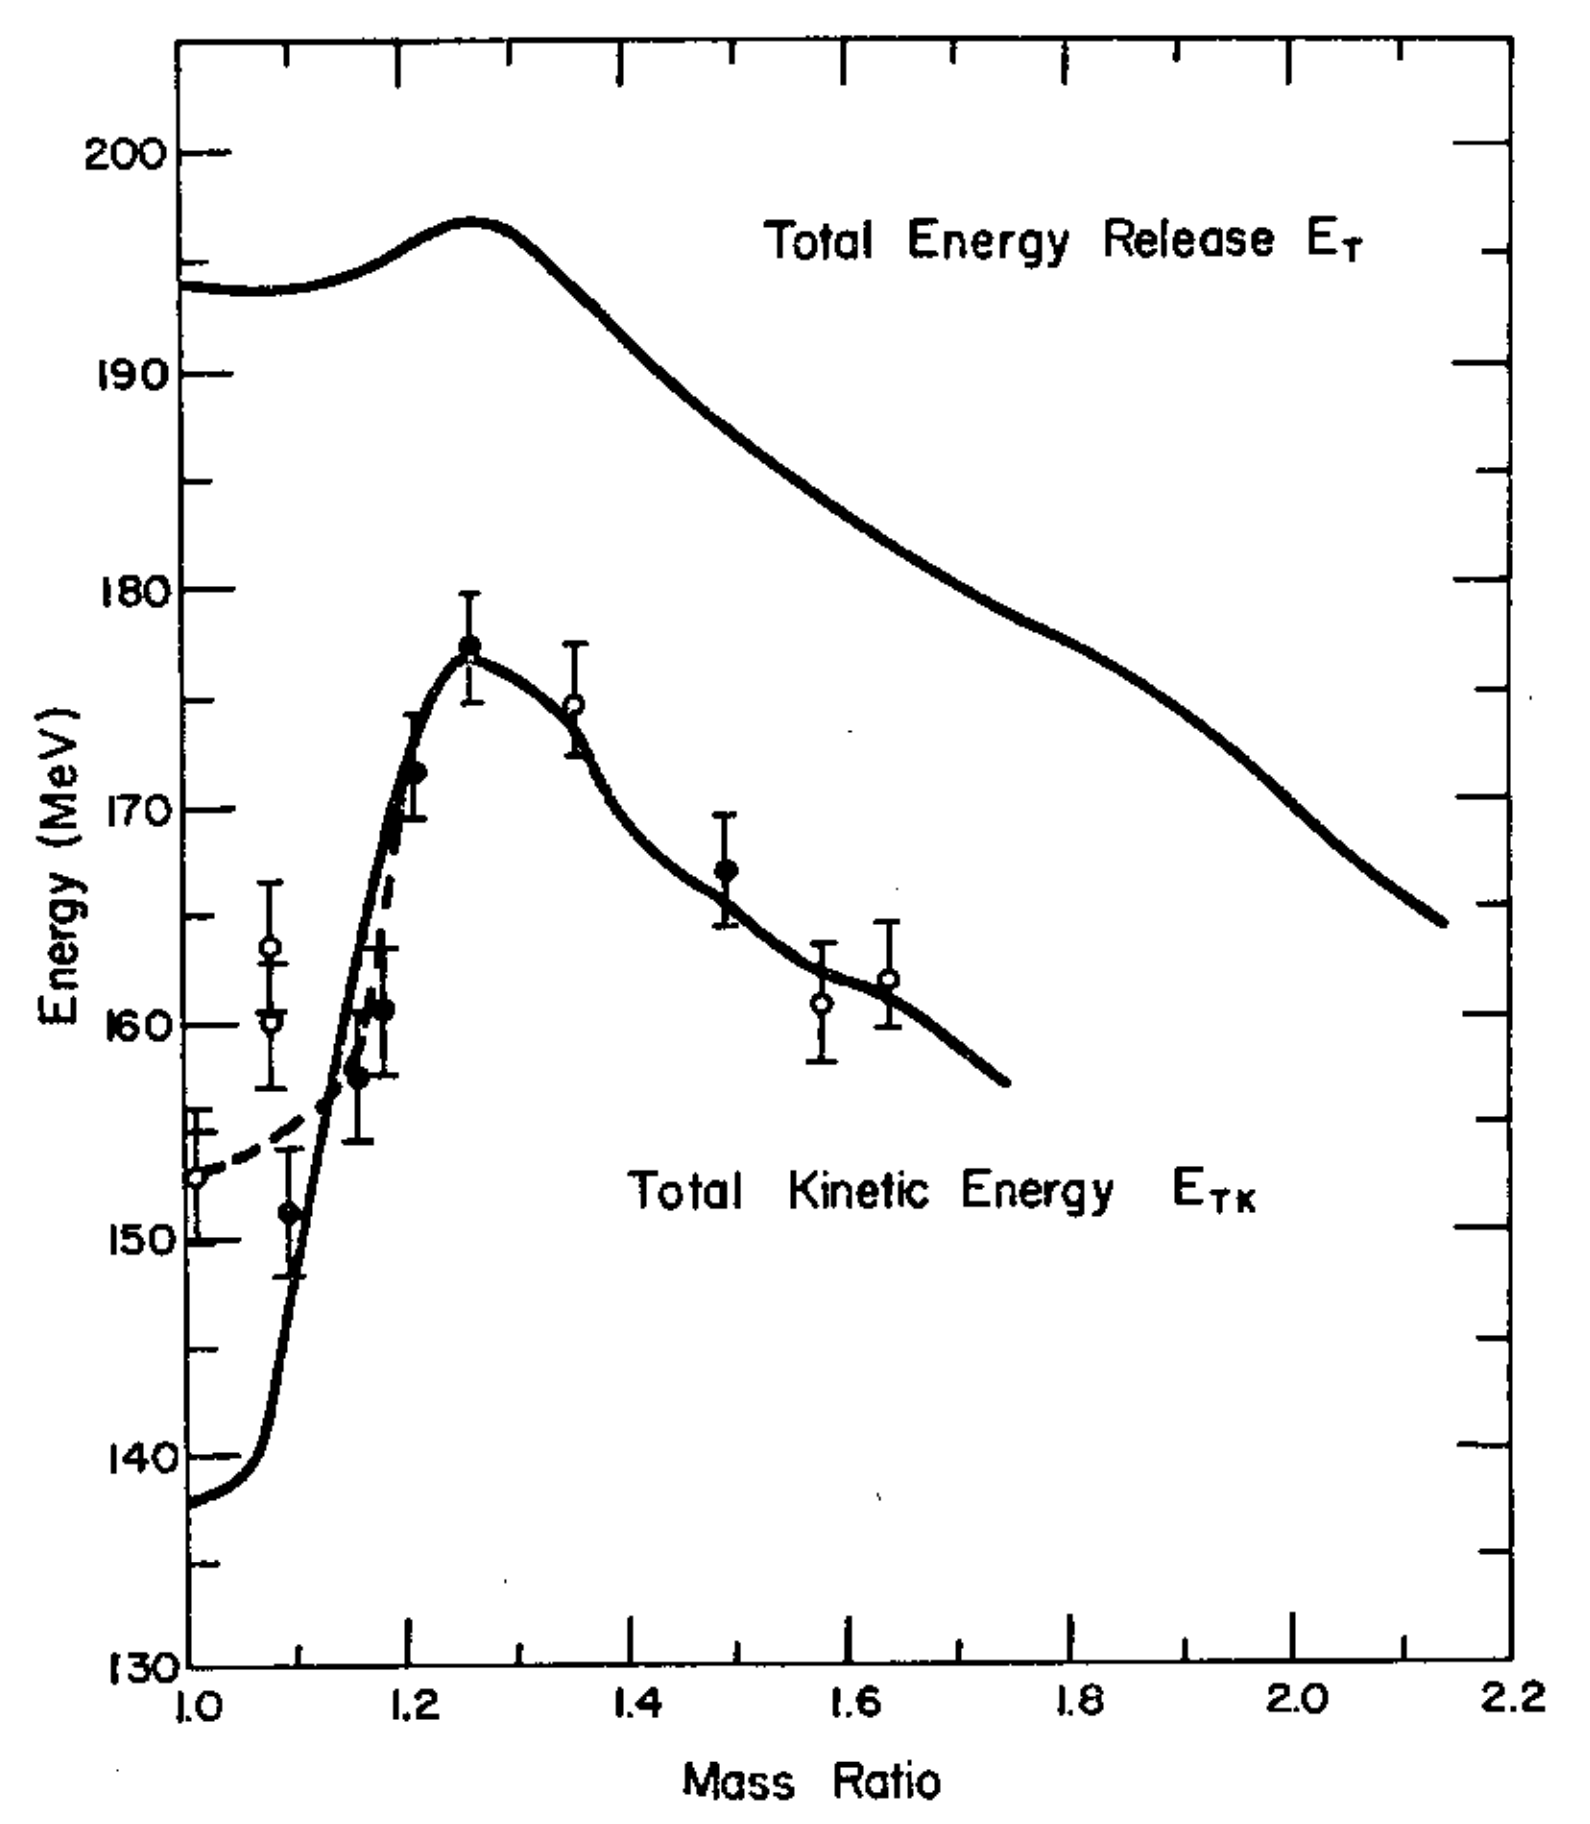
\includegraphics[height=11cm]{images/fission_energy_total.png}
\caption{Energy from thermal fission of U-235 as a function of mass ratios of child nuclei. Total energy release includes contributions from gamma rays and subsequent radioactive decays. Taken from \cite{aras1965ranges}.}
\label{figure:fissionenergy}
\end{figure}

Combustion-based power as a technology has matured over hundreds of years, with modern optimisations only looking to offer fractional percent gains in efficiency. By comparison, nuclear power technology is far from mature, with large improvements yet to be realised. One such feature is load-following, an enormously useful feature for a power plant which is currently unavailable in nuclear reactors. The biggest hurdle to achieving load-following in nuclear reactors is the issue of pellet-cladding interaction (PCI), which is the basis of the work in this thesis.

\subsection{Fission}

Commercial nuclear power plants extract energy through the process of fission, where a large nucleus is split into smaller nuclei. While it is also possible to extract energy from certain nuclei by the process of fusing them into larger ones, no fusion reactor currently exists which achieves a net positive energy output. At a fundamental level, both of these processes rely upon mass-energy equivalence. The relationship between mass and energy is shown using Einstein's famous equation:

\begin{equation}
\label{emc2}
    E = mc^{2}
\end{equation}

where $E$ is the energy of the system, $m$ is the mass and $c$ is the speed of light. Using this equation we can analyse a typical fission reaction:

\begin{equation}
\label{fission}
    U^{235}_{92} + n^{1}_{0} \longrightarrow I^{132}_{53} + Y^{101}_{39} + 3n^{1}_{0} 
\end{equation}

While the number of protons and neutrons are conserved throughout the reaction, a quick calculation will show that there is actually less mass in the products than the reactants by approximately 0.188 amu (3.127$\times 10^{-28}$ kg). This missing mass, known as the \emph{mass defect}, is converted to energy ($\sim$175 MeV). In this way, the total mass-energy of the system is conserved. 

This change in mass arises due to the phenomenon of \emph{binding energy}. In order for two or more nucleons to be thermodynamically stable when bound together, the total free energy of the bound configuration must be less than the sum of constituent nucleon free energies. Much like with energy stored in a chemical bond, the binding energy represents the energy required to separate the nucleus into individual protons and neutrons. 

Larger nuclei will generally have a greater total binding energy value compared to smaller nuclei, but the mass defect per nucleon will not necessarily be greater in a larger nucleus. It is therefore useful to normalise the binding energy by the mass number. Different isotopes have different binding energies, and any nuclear reaction which increases the binding energy per nucleon will be exothermic, whether by fission or fusion. Figure \ref{figure:bindingenergy} shows a plot of binding energy per nucleon against mass number with the relevant isotopes from Equation \ref{fission}. 

%235.0439299 + 1.008664 (236.0525939) -> 131.907997 + 100.93031 + 3.025992 (235.864299)



\begin{figure}[htp]
\centering
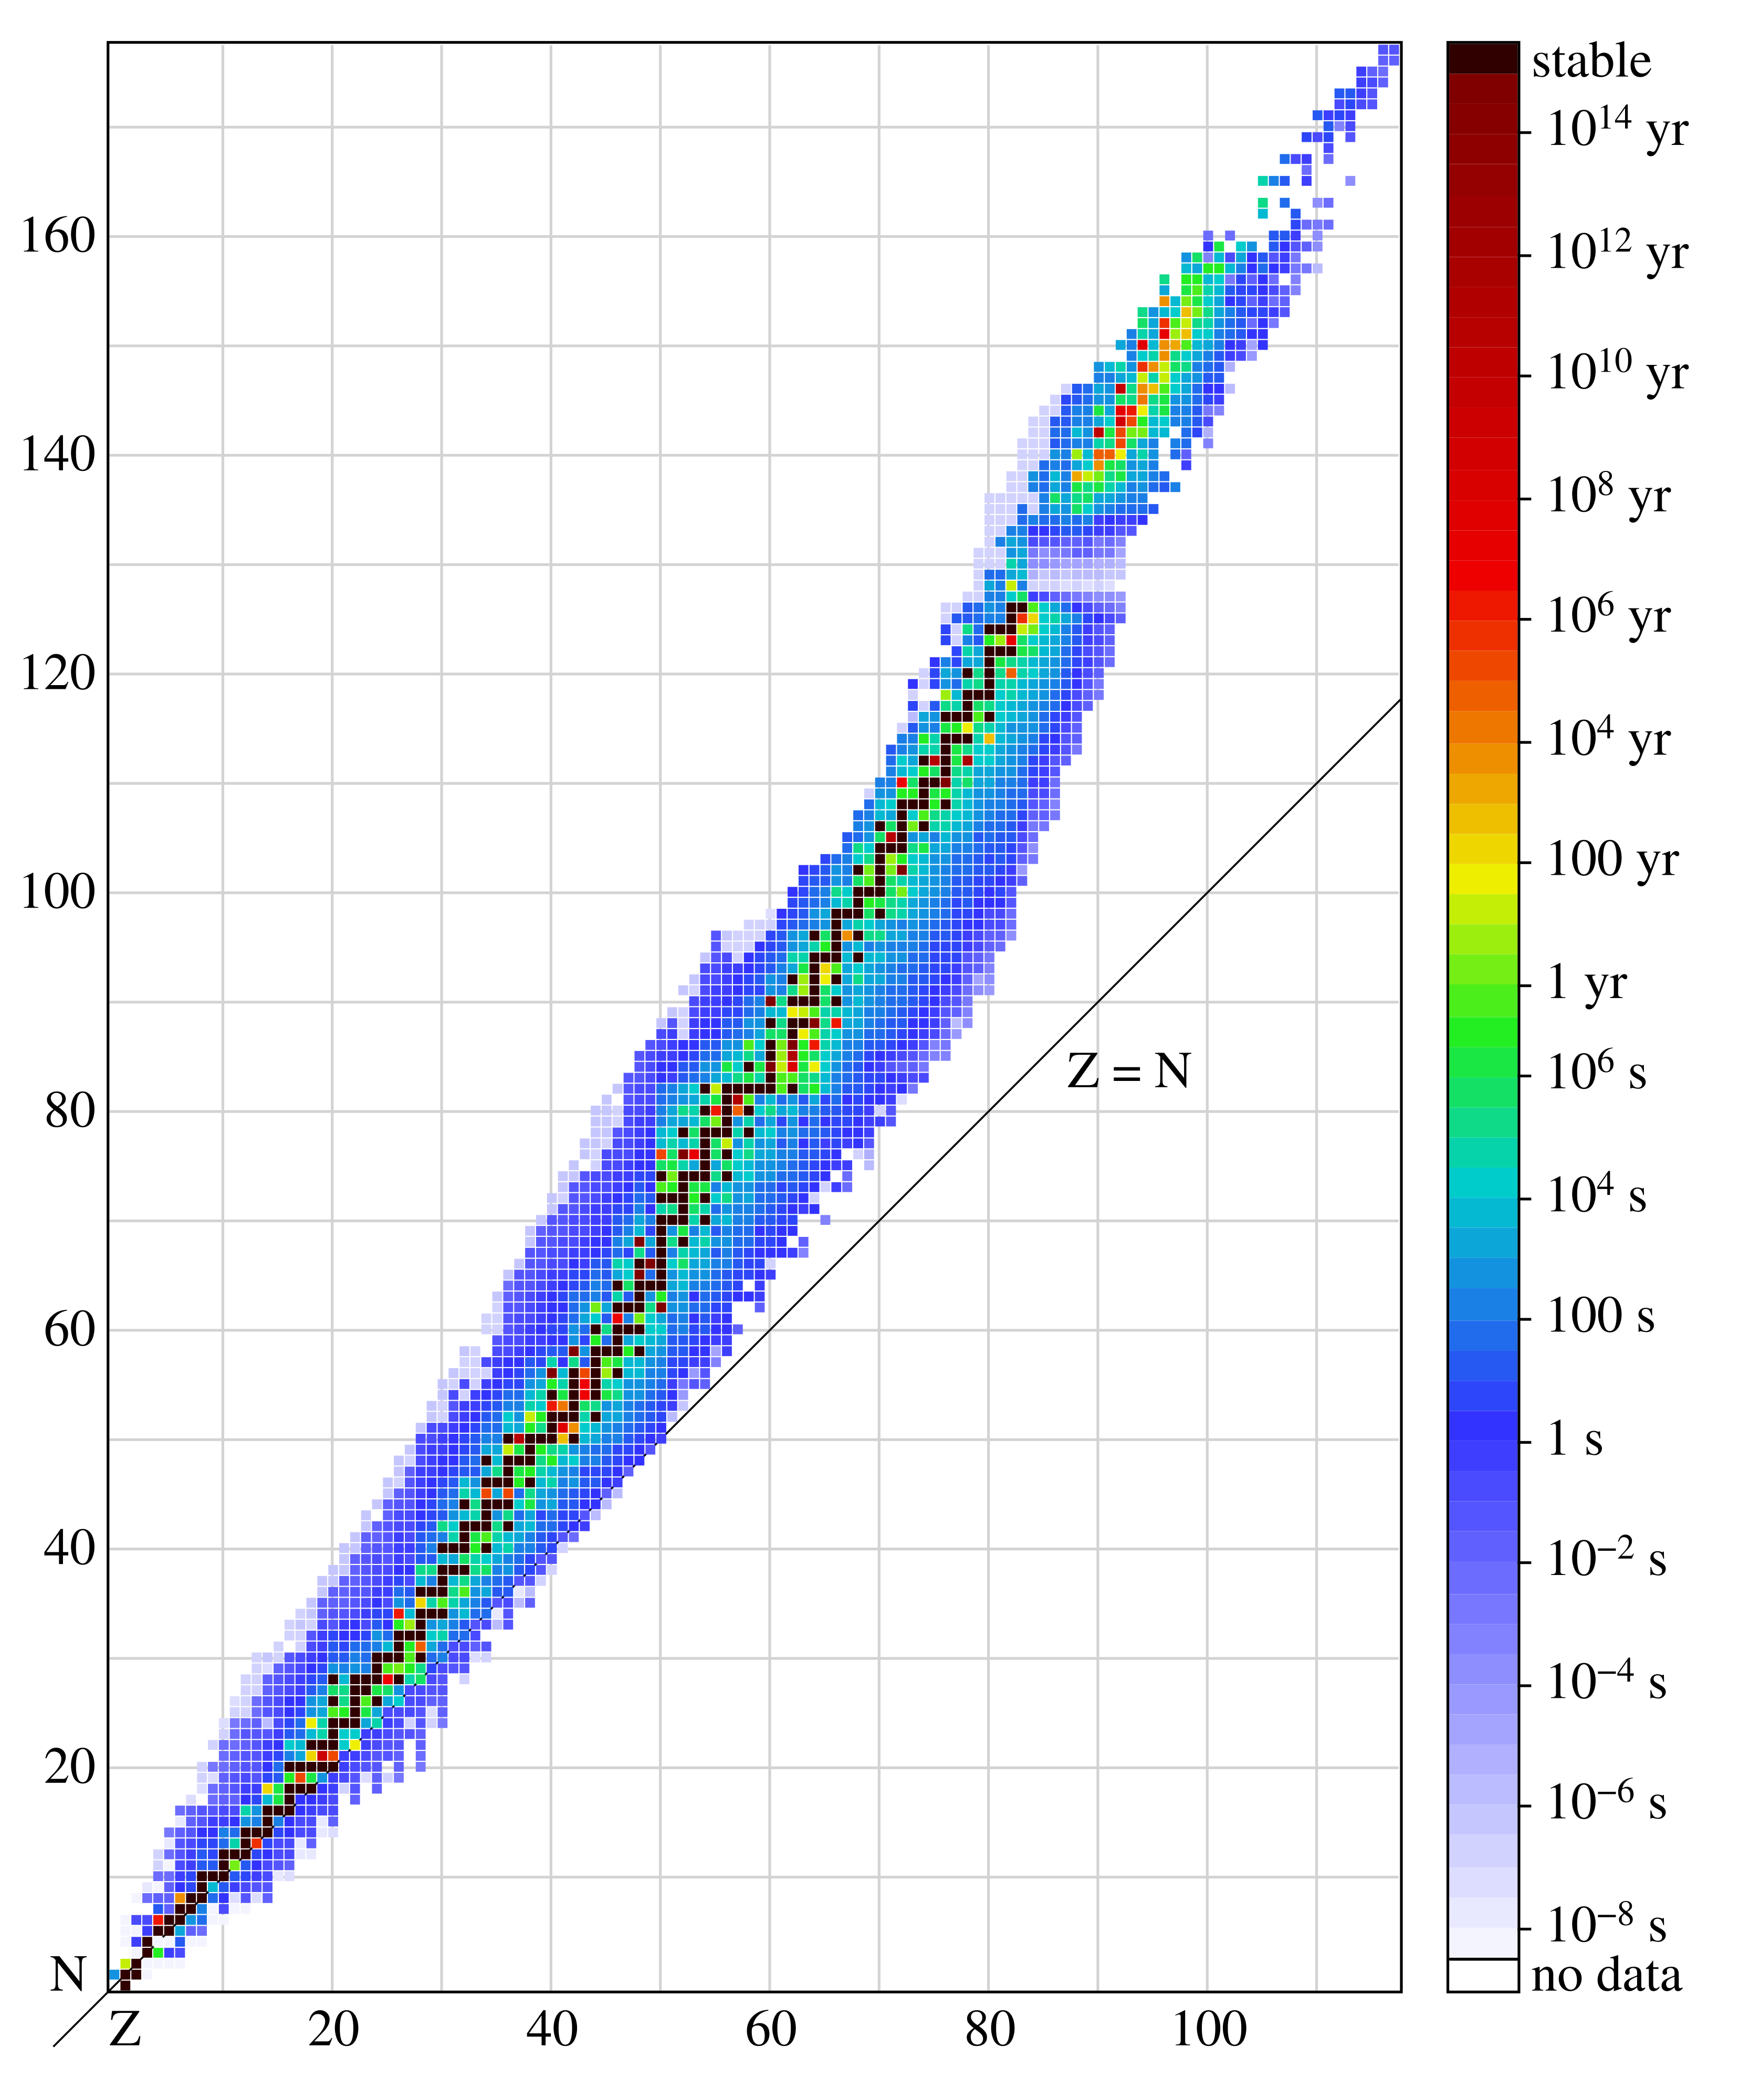
\includegraphics[height=11cm]{images/Isotopes_and_half-life.png}
\caption{Plot of neutron number against proton number for nuclei with half-lives greater than 10${^{-4}}$s. Half-life of the dominant decay mode is shown. Taken from \cite{BenRGPlotIsotopes}.}
\label{figure:NZcurve}
\end{figure}

\begin{figure}[htp]
\centering
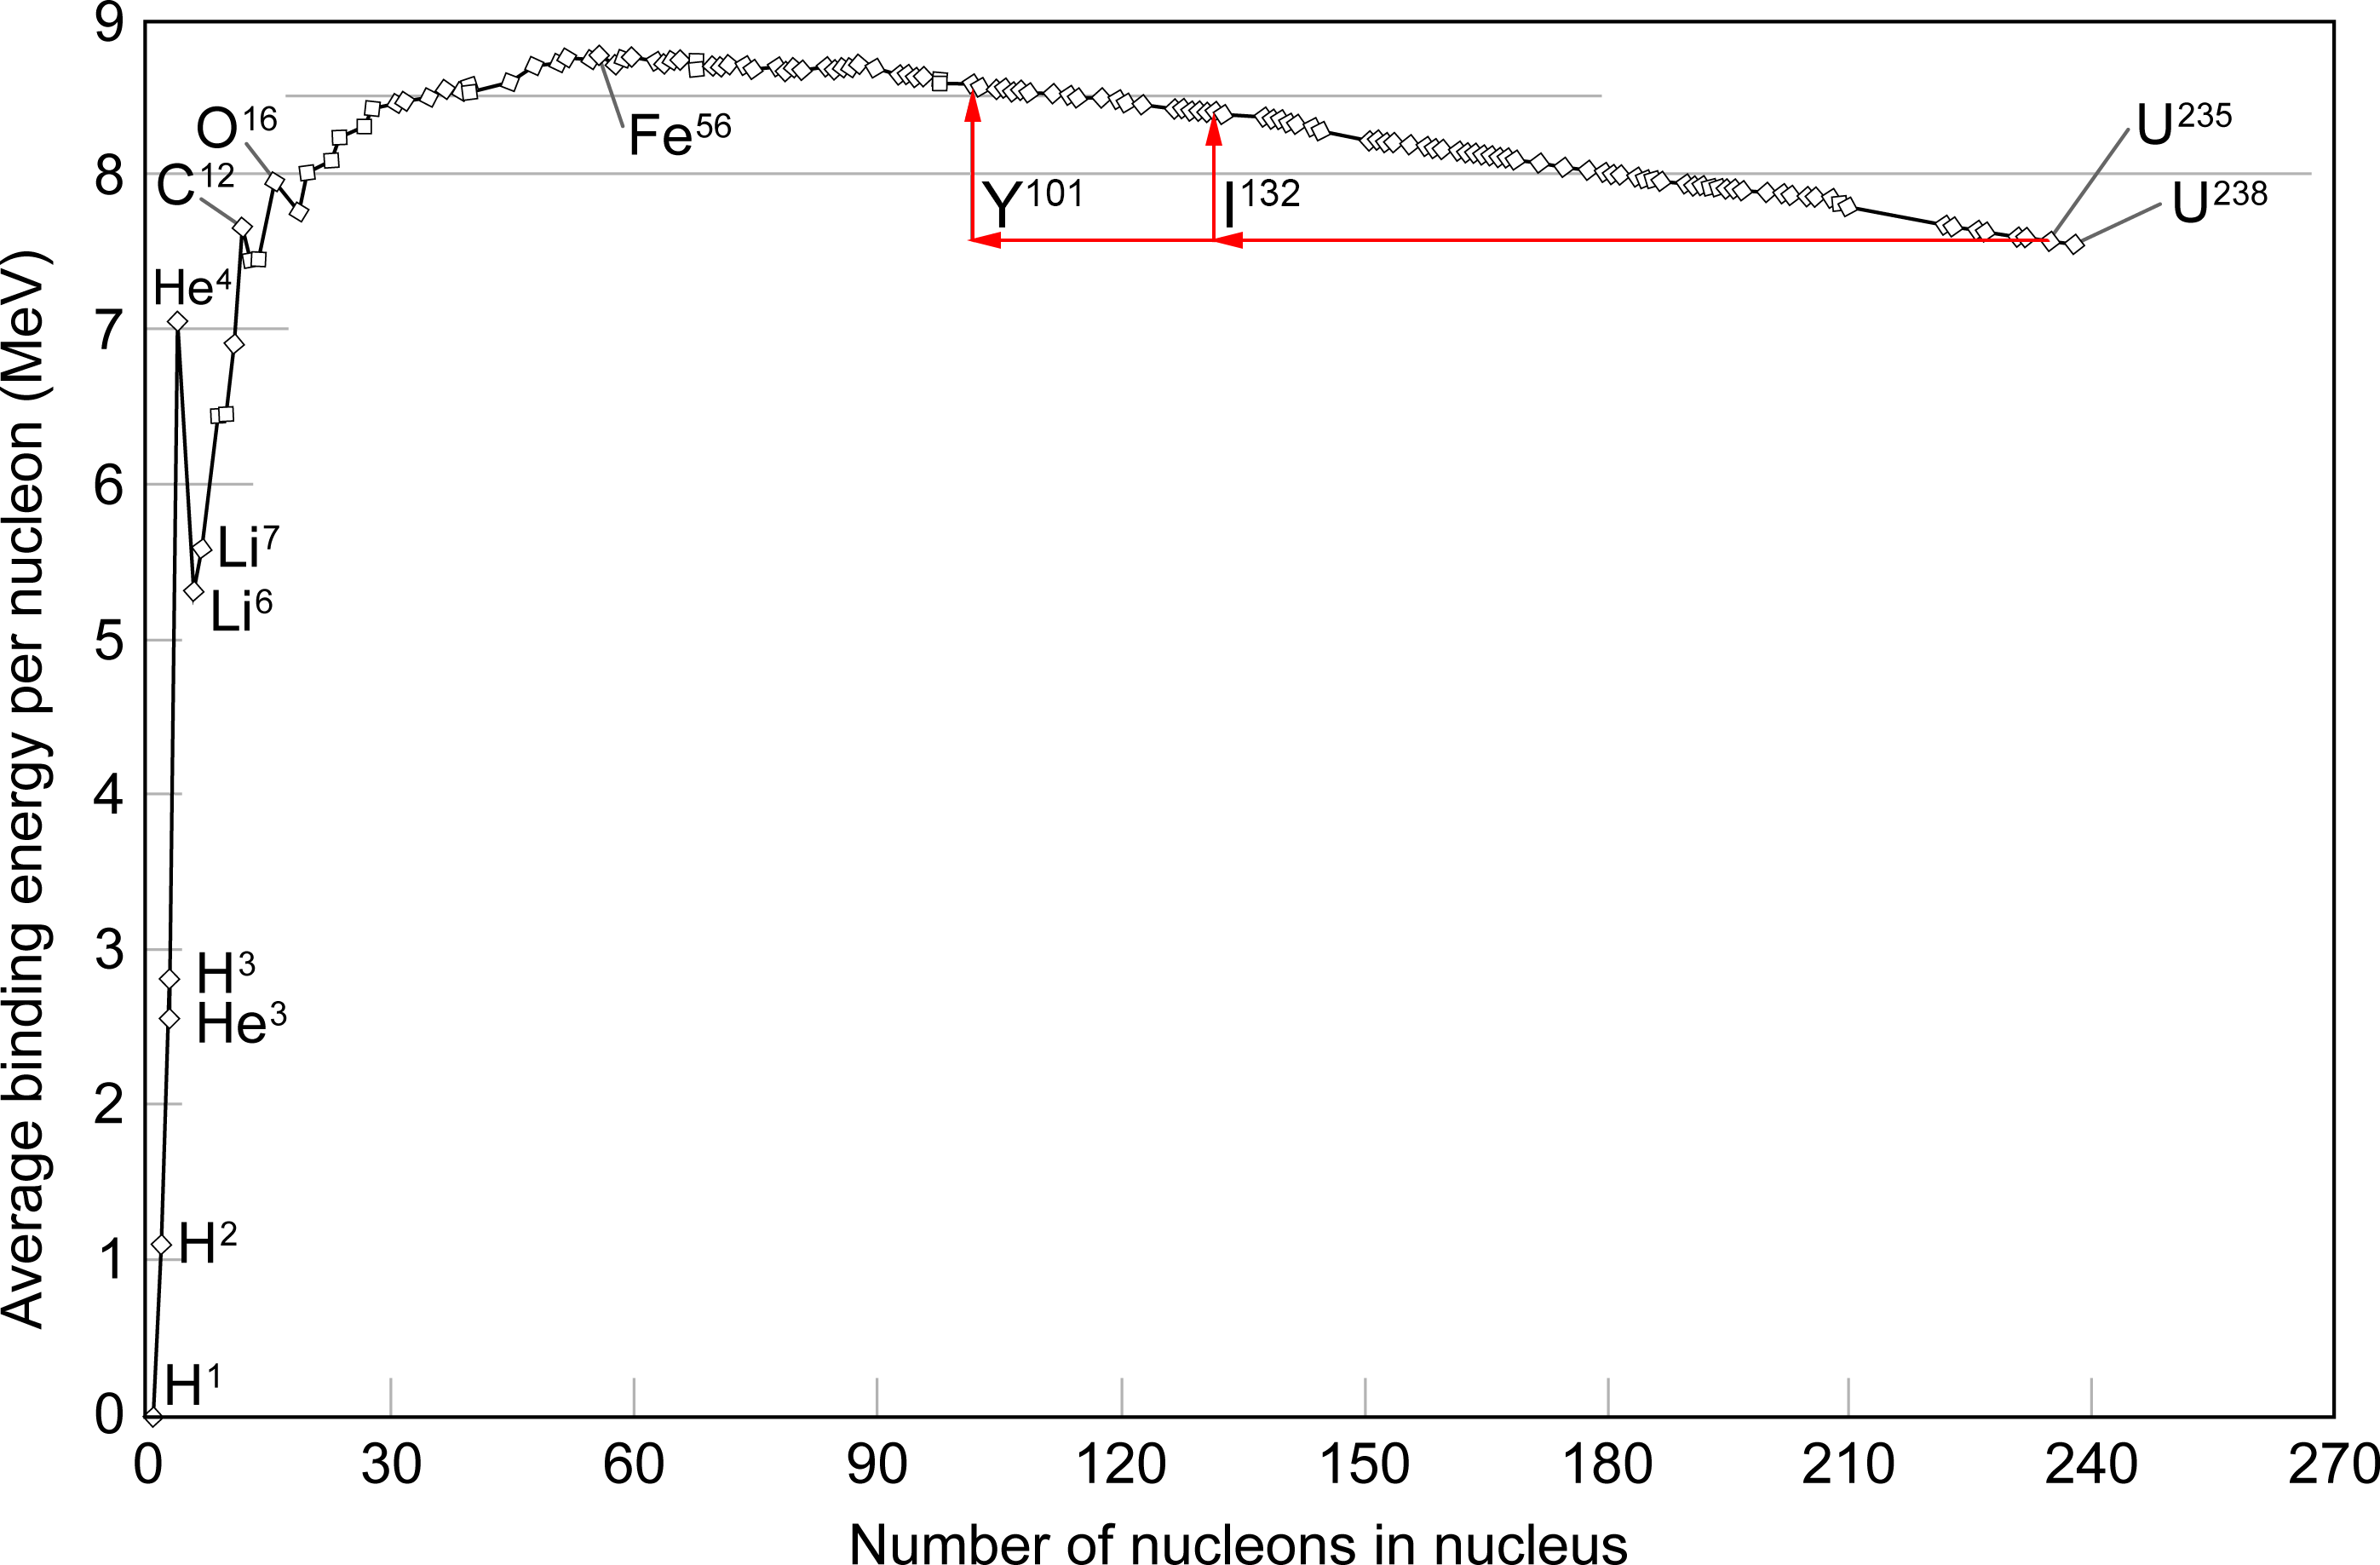
\includegraphics[height=11cm]{images/Binding_energy_curve.png}
\caption{Plot binding energy per nucleon against mass number. Arrows indicate the reaction shown in equation \ref{fission}. Adapted from \cite{FastfissionBindingCurve}.}
\label{figure:bindingenergy}
\end{figure}


\subsection{Reactor design}

Commercial nuclear reactors are large boilers in a Rankine cycle, designed to maximise heat transfer to a working fluid. All nuclear plants use steam turbines on the generation side, though the reactor coolant may be another fluid in a separate loop, such as carbon dioxide in gas-cooled reactors (GCRs), or even in a separate water loop such as in pressurised water reactors (PWRs) and CANDU. The work in this thesis is focused on zirconium-based claddings which are used worldwide in all commercial reactors except GCRs and sodium-cooled fast reactors. The most prevalent reactor type is the PWR, followed by the boiling water reactor (BWR) {REFER TO TABLE}. 


%Depending on the type of reactor, one or two coolant loops may be utilised. The generation side always involves 

\begin{itemize}
\item LWRs vs other kinds of reactors
\item Zirconium cladding used because of strength + low thermal neutron abs cross section
\item Thermal energy transferred from fuel to coolant
\item RPV is pressurised to 150 bar in PWRs, less in BWRs and even less in CANDU
\end{itemize}

\subsection{Nuclear reactor fuel pins}

Fuel assemblies in nuclear reactors are bundles of fuel pins. In most commercial reactors, these fuel pins are comprised of a zirconium-based cladding which is filled with UO$_{2}$ fuel pellets, each of which are approximately 1 cm$^{3}$ in volume. Once loaded with fuel pellets, the fuel pins are capped and filled with inert helium gas, pressurised to between 2 and 25 atm to improve heat transfer from the fuel pellets to the coolant as well as delaying inward creep deformation of the cladding due to the high coolant pressure \cite{King1980}. In the early stages of a fuel pin's life, there is a small gap between the fuel pellet and the cladding, known as the pellet-cladding gas gap. This gas gap slowly closes with increasing burn-up mostly due to swelling of the fuel pellets.

\subsubsection{Zirconium cladding}



\begin{itemize}
\item Zirconium cladding
\item Ceramic fuel pellets
\item Pellet-cladding gas gap
\item Cladding failure (great review here \cite{alam2011review})
\end{itemize}

\subsection{Effects of radiation on materials}

While ionising radiation is always present in the environment as background radiation, the intensity of radiation in a nuclear reactor is so great that it presents significant engineering challenges because of how it affects different materials.

Radiation hardening (also known as radiation embrittlement) is a phenomenon which affects most materials subjected to ionising radiation. It is characterised by a loss of plasticity caused by radiation damage over time, leading to an increased risk of cracks and failure of components. While zirconium is a very useful nuclear material due to it's neutron transparency, it is still susceptible to this type of damage \cite{Wisner1998CombinedZircaloy-2}. Beyond certain levels of radiation damage, phase changes may also occur. In \zirconia\ however,  

Amorphisation is another effect of radiation damage. This is characterised by a loss of long-range order of atoms in a crystal. This typically occurs beyond a certain threshold of radiation damage depending on the material, called the critical amorphisation dose. Amorphisation is problematic because the loss of a defined crystal structure results in both a reduction in structural stability (amorphous materials have a higher Gibbs free energy than their crystalline counterparts) and causes swelling of the material \cite{Einfal2013MethodsState}. In the literature, there is evidence of amorphisation in cubic stabilised \zirconia\ when bombarded with Cs$^{+}$ ions up to a fluence of $1 \times 10^{21}$ ions m$^{-2}$ \cite{amorphization2000wang}. However, no amorphisation is seen at an Xe$^{2+}$ fluence of $2 \times 10^{21}$ ions m$^{-2}$, or an I$^{+}$ fluence of $5 \times 10^{19}$ ions m$^{-2}$ \cite{sickafus1999radiation}.

One material phenomenon exclusive to nuclear reactor environments is neutron activation. The high free neutron environment leads to neutron capture in various nuclei within the reactor, including those of the fuel assemblies, coolant and RPV. There are many possible (n,x) reactions that may occur in materials experiencing a neutron flux, but of particular concern is transmutation of nuclei following a nuclear capture event. When a stable nucleus captures a neutron and becomes unstable, the nucleus may then emit particles to reduce it's free energy, altering it's atomic number in the process. This new element will have different chemical properties compared to the parent nucleus by virtue of a different electronic structure. This will change the elemental composition of a material, typically in an unfavourable way with dopants that negatively affect some desired material property. The extremely large number of nuclei relative to neutron flux means that this effect is small, though over time this becomes more significant due to accumulation of these dopant elements.

\begin{itemize}
\item Radiolysis
\end{itemize}

\subsection{Fission products, their distribution and decay chains}

\begin{itemize}
\item Bi-modal distribution of fission products due to binding energy gains (get a good binding energy per nucleon plot)
\item Fission products are almost always neutron-rich and will decay by beta-
\item Iodine is always paired with yttrium (53+39 protons). Yttrium happens to be a very good cubic phase stabiliser in \zirconia\ and decays into Zr.
\item Iodine appears both from direct fission, and from decay of tellurium which is also a common fission product.
\item The decay chain we are interested in is Te -> I -> Xe -> Cs
\end{itemize}

\section{Pellet-cladding interaction (PCI)}

PCI has been known about since 1974. Many studies and reviews have been made \cite{alam2011review}

\subsection{Effect of power ramps}
B.Cox PCI failures of Zr alloy fuel cladding \cite{bcoxpelletclad1990} talks about how they found out that fission products were necessary for PCI failures on page 260 (citation 54)

\subsection{Pellet-clad gap and bonding}

\begin{itemize}
\item At the beginning of life, there is a gas gap between the fuel pellet and the cladding, typically filled with an inert gas like helium during the manufacturing process.
\item With increasing burnup, radiation damage in the fuel pellet causes it to swell and therefore reduce the pellet-cladding gap, eventually making contact (and exerting a force) with the cladding.
\end{itemize}

\subsection{Iodine corrosion of zirconium}

\section{Oxidation of zirconium}

The oxidation of zirconium to produce \zirconia\ occurs during manufacture of the fuel clad when the metal is exposed to oxygen in air. \zirconia\ is a ceramic with material properties that make it desirable in many industrial applications, including solid-oxide fuel cells \cite{radford1979zirconia}, refractory linings \cite{whittemore1952fused}, and nuclear waste storage \cite{wang2012ceramics}.

\subsection{Oxygen solubility of zirconium}

\begin{itemize}
\item Oxygen is soluble in zirconium up to 29\% molar mass at "insert temperature".
\item Several PCI studies have assumed a mechanism whereby the \zirconia\ layer is fractured, allowing iodine to attack fresh metal surface, but these studies always assume that the exposed metal is oxygen-depleted.
\item It is not oxygen depleted, therefore they will always overestimate the amount of oxygen necessary to form a new passive oxide layer.
\end{itemize}

\subsection{Oxide growth mechanism}

An oxide layer will typically form on the surface of zirconium metal even at very low oxygen partial pressures \cite{causey2005review}. The oxidation process is mainly driven by the ingress of oxygen ions. Initially, the oxide is highly protective, growing slowly into the metal until it reaches a thickness of approximately 2-3 $\mu$m \cite{garzarolli1991oxide,dawson1968kinetics}, after which the oxide growth mechanism enters a `post-transition' stage where the oxidation kinetics follow a cubic-rate law  \cite{porte1960oxidation}.

\subsection{Outer oxide vs inner oxide}
The fuel cladding of an LWR develops an oxide on both the inner and outer surfaces due to exposure to oxygen in air during manufacture. 

\subsection{Sources of oxygen}

The internal oxide layer is present before fuel claddings are pressurised with helium gas and sealed. This is from the normal oxidation of Zr in air, where the oxygen pressure is 0.21 atm. After capping of the fuel rods, the only other available oxygen is from the UO$_{2}$ fuel pellets.

Uranium oxides have a wide range of non-stoichiometric compositions, with U/O ratios ranging from 1.67 to 2.24 in solid UO$_{2 \pm x}$, as shown in Figure \ref{figure:U_O_phase_diagram}. The oxide form U$_{3}$O$_{8-y}$ also exists and is more kinetically and thermodynamically stable than UO$_{2}$, but has lower density, making it less suitable for use as a fuel form. The different stoichiometries have different equilibrium O$_{2}$ pressures at constant temperature (REF TABLE), allowing some level of tweaking the internal cladding environment depending on whether more or less oxygen is desired. 

Oxygen and oxygen precursors may also be produced directly from fission of U
$_{235}$, but this contribution is insignificant compared to changing the stoichiometry of the fuel pellet. Indeed, liberation of oxygen from UO
$_{2 \pm x}$ due to fission (which is also a function of the fuel's stoichiometry) is a more significant contributor to the oxygen pressure than direct production via fission.

\begin{figure}[htp]
\centering
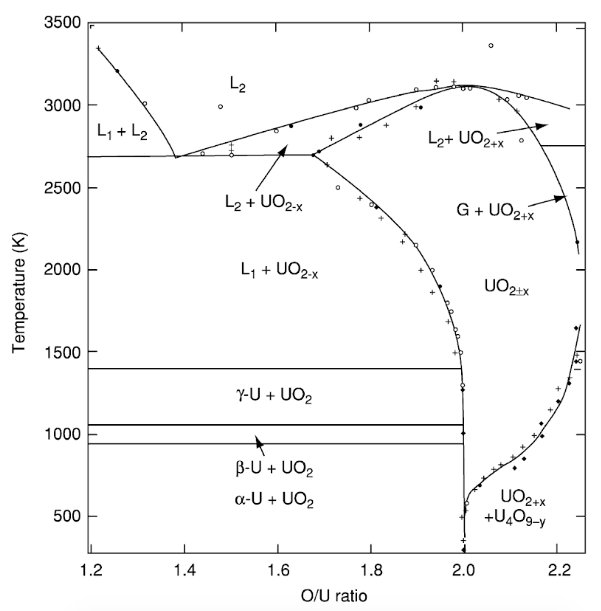
\includegraphics[height=11cm]{images/UO_phase_diagram.png}
\caption{Partial U-O temperature phase diagram between O/U ratios of 1.2 and 2.25. Figure taken from \cite{katz2007chemistry}, with phase boundaries from \cite{rand1978thermodynamic, chevalier2002progress, gueneau2002thermodynamic}.}
\label{figure:U_O_phase_diagram}
\end{figure}


\begin{figure}[htp]
\centering
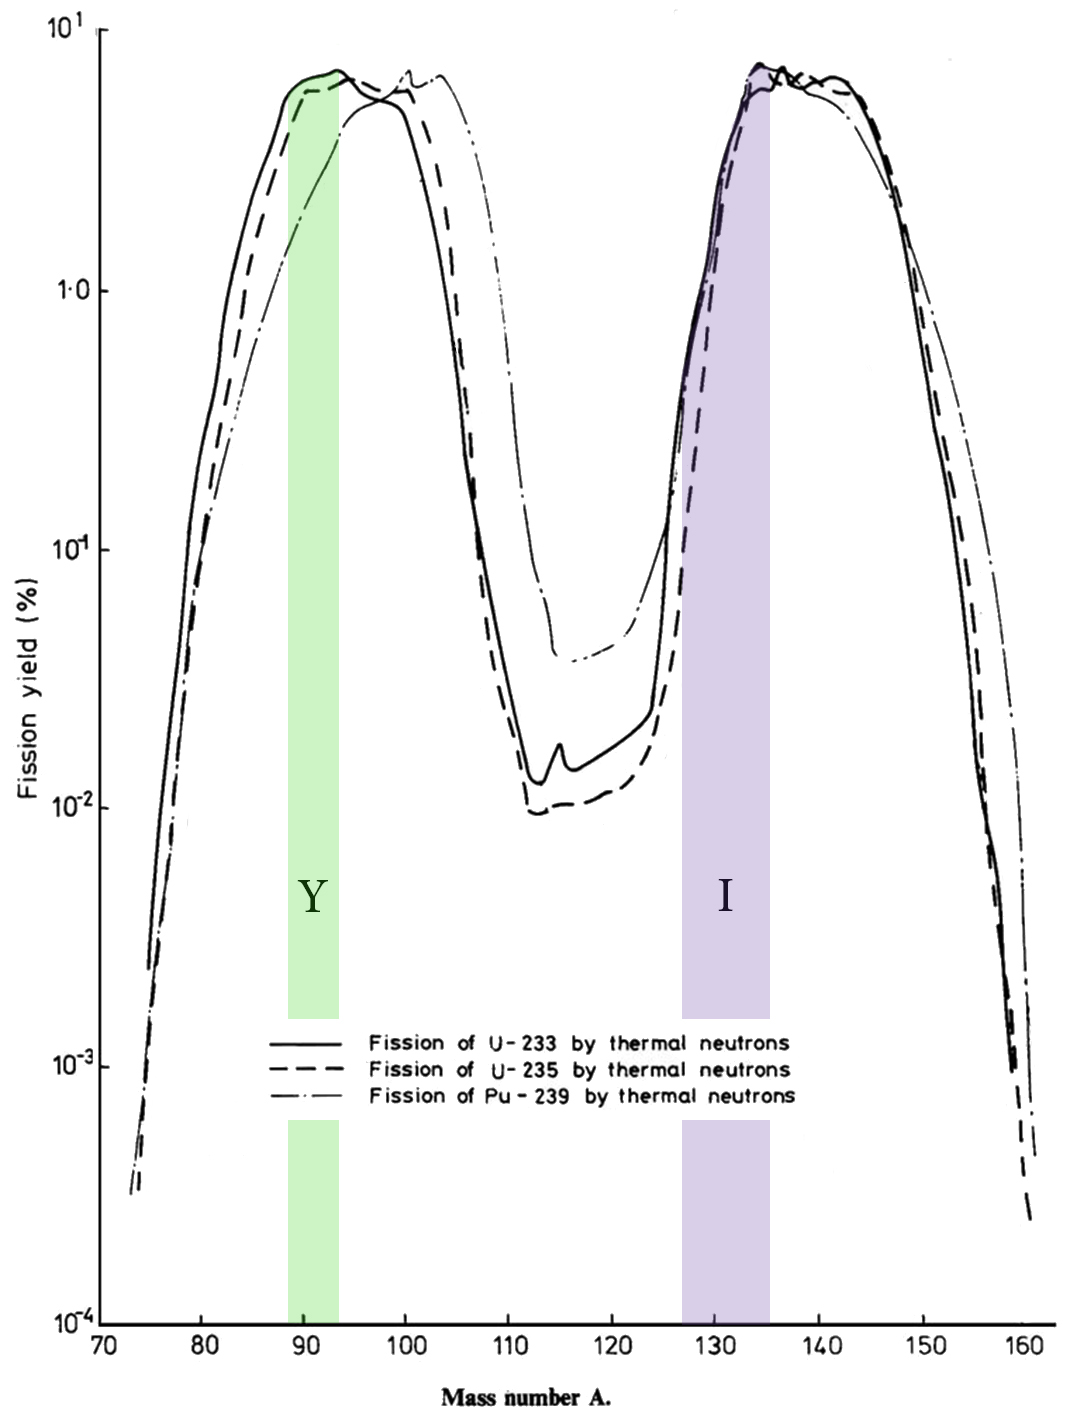
\includegraphics[height=11cm]{images/fissionyield.jpg}
\caption{Plot of the percentage yield of nuclei with a given mass following a fission event. Range of masses corresponding to isotopes of iodine shown in purple and isotopes of yttrium shown in green.}
% M. F. James, R. W. Mills and D. R. Weaver (1991) UKAEA Reports, AEA-TRS-1015, AEA-TRS-1018 
         %  and AEA-TRS-1019.
\label{figure:fissionyield}
\end{figure}

\section{Atomistic Simulation}

\subsection{Classical approach - molecular dynamics}

\begin{itemize}
\item Molecular dynamics allows for large system sizes (millions of atoms) compared to DFT because of the low computational cost of classical potentials. 
\item These are mainly pair potentials (although many-bodied potentials are also used) which are some combination of a short-range repulsion term (Pauli exclusion, nuclear repulsion if van der waals is taken into account) and a long range Coulombic attraction term
\end{itemize}

\subsection{Quantum mechanical approach - DFT}

\begin{itemize}
\item Up to hundreds of atoms, but far more fundamental data such as electron density.
\item Very computationally expensive, but with clever workarounds for bulk crystallographic systems.
\end{itemize}

\subsection{Band gap}

Materials are sometimes considered to fall into one of two categories; conductors or insulators. While this binary characterisation may work as an approximation for many materials, in reality there is more of a continuum between these two states, and at the heart of this lies the band gap.

It is known that for ions, electron energy levels are quantised, restricting the range of possible electron energies to discrete quantities. More specifically, electrons can only occupy unique quantum states, defined by parameters such as quantum spin and angular momentum. In a crystal, where there are large numbers of electrons and many possible configurations of them, we refer to energy "bands" which are comprised of many quantised energies. There are sometimes gaps between energy bands in crystals corresponding to energy levels that cannot be occupied, meaning that if electrons were to be added at the lowest energy levels one by one, there would occasionally be relatively large jumps in energy as an electron is forced to enter a higher energy band. 

Two energy bands, called the valence band and conduction band, help determine a material's metallic or non-metallic character. The valence band contains energy levels occupied by the valence electrons (at absolute zero), while the conduction band contains energy levels which are high enough that electrons may freely move throughout the crystal. In metals, the valence and conduction bands have some amount of overlap, meaning that once the valence band is full, the highest occupied electron energy states are within the conduction band and so the material acts as a conductor. Materials like \zirconia , however, have large energy gaps between the valence and conduction bands, known as the band gap. These materials are called "band insulators" (as opposed to Mott insulators), because the band gap is an energy barrier preventing the valence electrons from moving freely around the crystal.

In addition to the valence and conduction bands, we also need a value for the electron chemical potential or Fermi level of the material to determine how the energy bands are filled. 

\begin{figure}[htp]
\centering
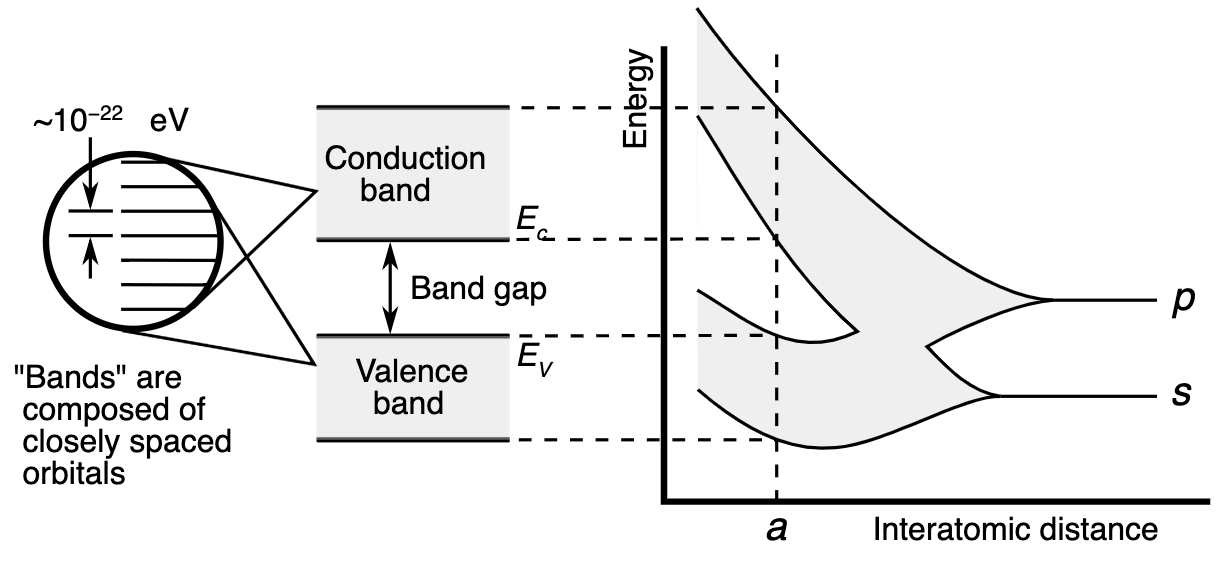
\includegraphics[width=\linewidth]{images/band_gap.png}
\caption{Illustration of the band gap in diamond as a function of interatomic spacing. Taken from \cite{Chetvorno2017}.}
\label{figure:band_gap}
\end{figure}

\begin{itemize}
\item In a crystal, large numbers of electrons and many possible configurations lead to electron energy 'bands' made up of many quantised energies (electron band theory). See http://hyperphysics.phy-astr.gsu.edu/hbase/Solids/band.html
\item Non-metals exhibit an energy gap between valence and conduction electron bands, demarcating insulators and conductors.
\end{itemize}

\begin{figure}
\begin{center}
\begin{tikzpicture}
	\begin{axis}
		[width=11cm, xlabel={Energy (eV)}, ylabel={Electronic density of states}, ymin=0, ymax=12, xmin=0, xmax=16, legend style={{draw=}, at={(0.05,0.95)}, anchor=north west, legend columns=1}]
% 		\addplot[no marks] table [x=log(pO2)/atm, y=Electrons,]{tetintrinsic.dat}; \addlegendentry{e\SPSB{$\prime$}{}};
%         \addplot[no marks, dashed] table [x=log(pO2)/atm, y=Holes, ]{tetintrinsic.dat}; \addlegendentry{h\SPSB{\textbf{\textperiodcentered}}{}};
%         \addplot[no marks, densely dotted, red] table [x=log(pO2)/atm, y=VO+2,]{tetintrinsic.dat}; \addlegendentry{V\SPSB{\textbf{\textperiodcentered\textperiodcentered}}{O}};
%         \addplot[no marks, dashed, red] table [x=log(pO2)/atm, y=VO+1,]{tetintrinsic.dat}; \addlegendentry{V\SPSB{\textbf{\textperiodcentered}}{O}};
%         \addplot[no marks, red] table [x=log(pO2)/atm, y=VO0,]{tetintrinsic.dat}; \addlegendentry{V\SPSB{$\times$}{O}};
%         \addplot[no marks, densely dotted, blue] table [x=log(pO2)/atm, y=VM-4,]{tetintrinsic.dat}; \addlegendentry{V\SPSB{$\prime\prime\prime\prime$}{Zr}};
%         %\addplot[no marks, dashed, blue] table [x=log(pO2)/atm, y=VM-3,]{tetintrinsic.dat}; \addlegendentry{V\SPSB{$\prime\prime\prime$}{Zr}};
       \addplot[no marks] table [x=mono_x, y=mono_y,]{dat/eDOS.dat}; \addlegendentry{Monoclinic};
       \addplot[no marks, dashed] table [x=tet_x, y=tet_y,]{dat/eDOS.dat}; \addlegendentry{Tetragonal};
       \addplot[no marks, densely dotted] table [x=cubic_x, y=cubic_y,]{dat/eDOS.dat}; \addlegendentry{Cubic};

			\end{axis}
		\end{tikzpicture}
		\caption{Electronic density of states for the different crystal structures of \zirconia\ showing the band gap predicted by DFT.}
		\label{figure:densityofstates}
	\end{center}
\end{figure}

\begin{table}[htp] % Band Gap
\onehalfspacing
\centering
\caption{Experimentally determined band gaps alongside values calculated from DFT simulations for each crystal structure of zirconia. Experimental values taken from \cite{French1994}.}
\begin{tabular}{ccc}
{\bf }                                       & \multicolumn{2}{c}{{\bf Band gap (eV)}}      \\ \hline
\multicolumn{1}{c}{{\bf Crystal Structure}} & \multicolumn{1}{c}{{\bf Expt.}} & {\bf DFT} \\ \hline
\multicolumn{1}{c}{Monoclinic}              & \multicolumn{1}{c}{5.83}        & 3.45      \\
\multicolumn{1}{c}{Tetragonal}              & \multicolumn{1}{c}{5.78}        & 4.00      \\
\multicolumn{1}{c}{Cubic}                   & \multicolumn{1}{c}{6.10}         &   3.55 \\ \hline
\label{table:bandgap}
\end{tabular}
\end{table}


 % Complete
\chapter{Literature Review}

\label{literature_review}

\section{Pellet-cladding interaction (PCI)}

At the beginning of a fuel pin's life, there is a gap between the fuel pellet and the cladding (see \ref{ss_fuelpin}). This gas gap slowly closes over time, mostly due to thermal expansion and swelling of the fuel pellet (illustrated in Figure \ref{figure:pcmi}) due to radiation damage. At a high enough burnup, the fuel pellet finally makes contact with the cladding. This phenomenon is called pellet-cladding interaction (PCI) and involves both mechanical and chemical interactions which contribute to observed fuel failures.

\begin{figure}[ht]
\centering
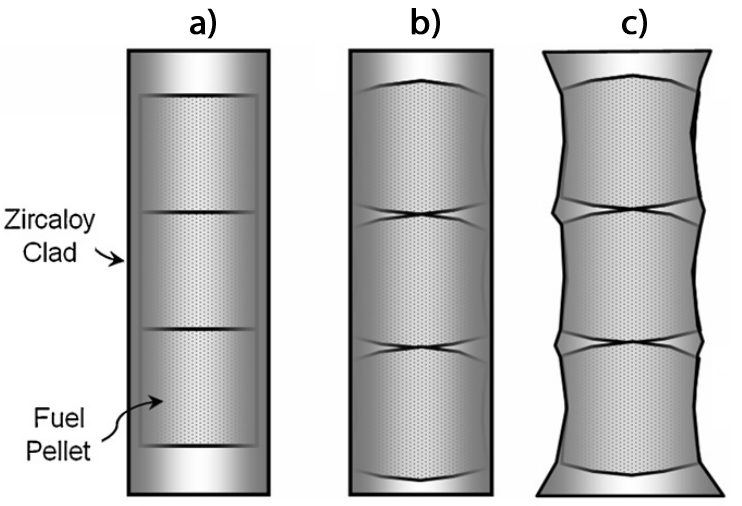
\includegraphics[height=9cm]{images/pcmi.png}
\caption[Illustration of fuel swelling and clad deformation due to PCI.]{Illustration of fuel swelling and clad deformation due to PCI. Adapted from \cite{alam2011review}.}
% M. F. James, R. W. Mills and D. R. Weaver (1991) UKAEA Reports, AEA-TRS-1015, AEA-TRS-1018 
         %  and AEA-TRS-1019.
\label{figure:pcmi}
\end{figure}

PCI-related failure of nuclear fuel pins has been known about since 1963, when the first reported failure occurred in a highly rated fuel pin during reactor start-up \cite{lyons1963high}. Many studies have since been made on the topic \cite{alam2011review, bcoxpelletclad1990}. The exact cause of PCI failures has not yet been discovered, however it is likely that both the mechanical and chemical effects of contact between the fuel pellet and the cladding are necessary. It is also known that PCI failures are typically preceded by power transients, such as during reactor startup where several power ramps are performed over many hours.

\subsection{Pellet-clad gap and bonding}

The gap between the fuel and the cladding allows fuel pellets to be inserted into the fuel pin easily during manufacture, but this clearance is also designed to accommodate some increase in fuel pellet volume. It is important to consider the thermal expansion of the fuel pellet, as the centreline temperature of a PWR fuel pellet during a power transient can vary between 1500 and 1800 $^{\circ}$C, depending on the burnup of the fuel and magnitude of the reactivity insertion \cite{Bagger1994}. In addition, fuel pellets will swell due to radiation damage throughout their operational lifetime. Once the pellet-clad gap has closed entirely, any pellet expansion during a power transient will translate to a force exerted on the cladding, generating hoop stresses which open cracks on the inner cladding surface. This is the mechanical component of PCI.

When the fuel pellet makes contact with the cladding, there is also a chemical interaction between the UO$_{2}$ (and fission products) and the internal surface oxide of the cladding. UO$_{2}$ has some solubility in ZrO$_{2}$, and we therefore see a bonded reaction layer, which is of the form (U, Zr)O$_{2}$.  Due to the large U atom, cation substitution allows this mixed layer to adopt the crystal structure of cubic fluorite, the high temperature phase of ZrO$_{2}$. The uranium nuclei in both this bonding layer and the outer rim of the fuel pellet experience the highest number of fission events (due to proximity to the moderator), and therefore this region contains fission products that contribute to the chemical degradation of the fuel cladding, such as iodine. This is the chemical component of PCI.

\subsection{Reactor power ramps}

It has been firmly established that power ramping of the reactor is associated with PCI failures \cite{penn1977candu, MacDonald1979, Hardy1977198, Knaab1987}. This presents a problem for reactors when it comes to events such as start-up, load-following and any other power transients experienced by the fuel pins. Figure \ref{figure:reactor_startup} shows how reactor power varies over time during a typical PWR start-up procedure. A combination of low ramping rates and long holds at low power (to remain below ramping limits, to condition fuel \cite{billaux2005pellet} \footnote{Fuel is considered `conditioned' after it has operated at a specified power level for a certain period of time.}, and conduct coolant chemistry checks) require the entire procedure to be completed in a period of 90 hours, with several operator switch-overs in between. This is a costly procedure for the utility owner to perform, with millions of US\$ foregone in electricity sales for bigger reactors, of which there are typically two or more per power plant. 

\begin{figure}[ht]
\centering
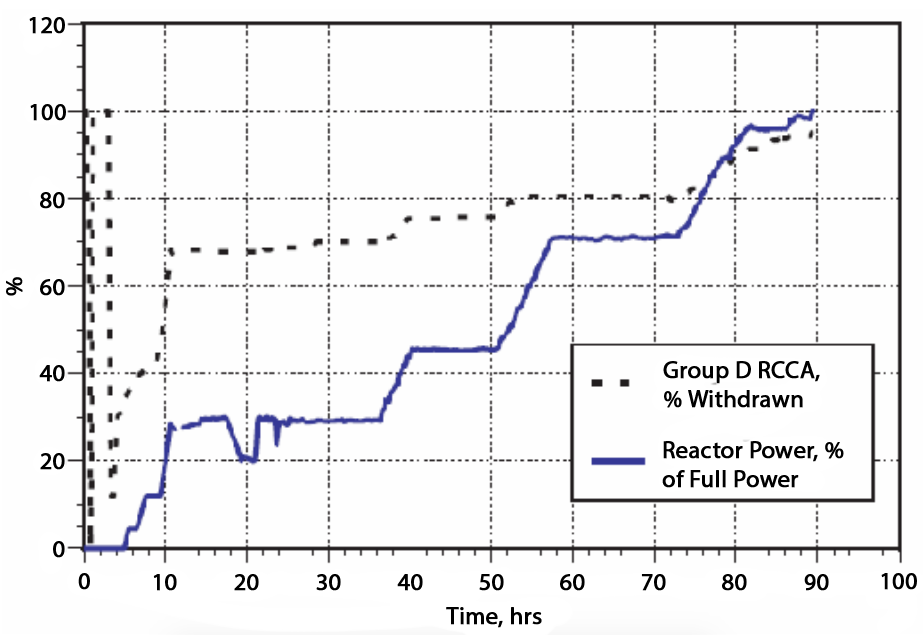
\includegraphics[height=10cm]{images/reactor_startup.png}
\caption[Reactor startup procedure for a typical US PWR. Dashed line indicates \% withdrawal of control rods.]{Reactor startup procedure for a typical US PWR. Dashed line indicates \% withdrawal of control rods. Adapted from \cite{ramping}.}
% M. F. James, R. W. Mills and D. R. Weaver (1991) UKAEA Reports, AEA-TRS-1015, AEA-TRS-1018 
         %  and AEA-TRS-1019.
\label{figure:reactor_startup}
\end{figure}

Scheduled reactor shutdowns or extended reduced power operation (ERPO) events occur whenever refuelling or maintenance of the reactor is required (and in some cases there may be a grid demand to reduce power output).  Refuelling is typically performed every 1 to 2 years, while maintenance may be required at any time. Emergency shutdowns may also occur and have their own challenges to consider (e.g. xenon poisoning, decay heat removal), though they are more rare. In each case, going through the lengthy power ramping procedure is required, and since these shutdowns cannot be avoided, being able to ramp up power faster would be a significant improvement. Ramp rates in reactors are restricted to between 3-4\% of full power per hour above a certain threshold level to avoid PCI failures \cite{ramping}. Additionally, fuel conditioning holds (operation at certain power levels for long periods) are performed to further reduce the incidence of PCI failures. 

These limits present a challenge not just when restarting reactors, but also for the implementation of load-following in reactors. PWRs have thermal feedback loops which provide some level of intrinsic load-following behaviour. For example, an increase in steam demand leads to increased boiling in the steam generators. The subsequent decrease in temperature of coolant in the primary circuit leaving the steam generator causes a reactivity increase and therefore a power increase in the reactor. The reactor returns to critical (reactivity = 0) after some fluctuation, and the average temperature of the coolant remains unchanged.

\subsection{Fission products and SCC}

Although PCI failures were found to occur during power ramping, it was not yet known whether these failures were due to fission product induced SCC or tensile failure of the cladding due to radiation embrittlement. 

In 1971, scientists at the Chalk River Nuclear Laboratories conducted a series of tests to determine if fission products were necessary \cite{MacDonald1979}. The experiments involved taking highly irradiated zirconium fuel pins (fluence of $8 \times 10^{24}$ n/m$^{2}$ with 1 MeV neutrons) and then inserting fresh, unirradiated UO$_{2}$ fuel pellets into them. These fuel pins were then inserted back into a reactor and subjected to large power ramps, as shown in Figure \ref{figure:fueltests}. These ramps (phase I and II) would typically cause failures in fuel pins with similar irradiation histories. In the initial ramp tests however, all the fuel pins survived the ramps intact. Six fuel pins were then irradiated in the reactor at low power to a burnup in excess of 50 MWh/kg U in order to build up fission products in the fuel (phase III). In a subsequent ramp test (phase IV), two of the high burnup fuel pins failed in the reactor. This finding provided the strongest evidence to date that fission products are necessary for PCI failure of zirconium-based claddings. The fission product most likely to cause cracking, based on known SCC susceptibility of Zr metal, is iodine.

\begin{landscape}
\begin{figure}[ht]
\centering
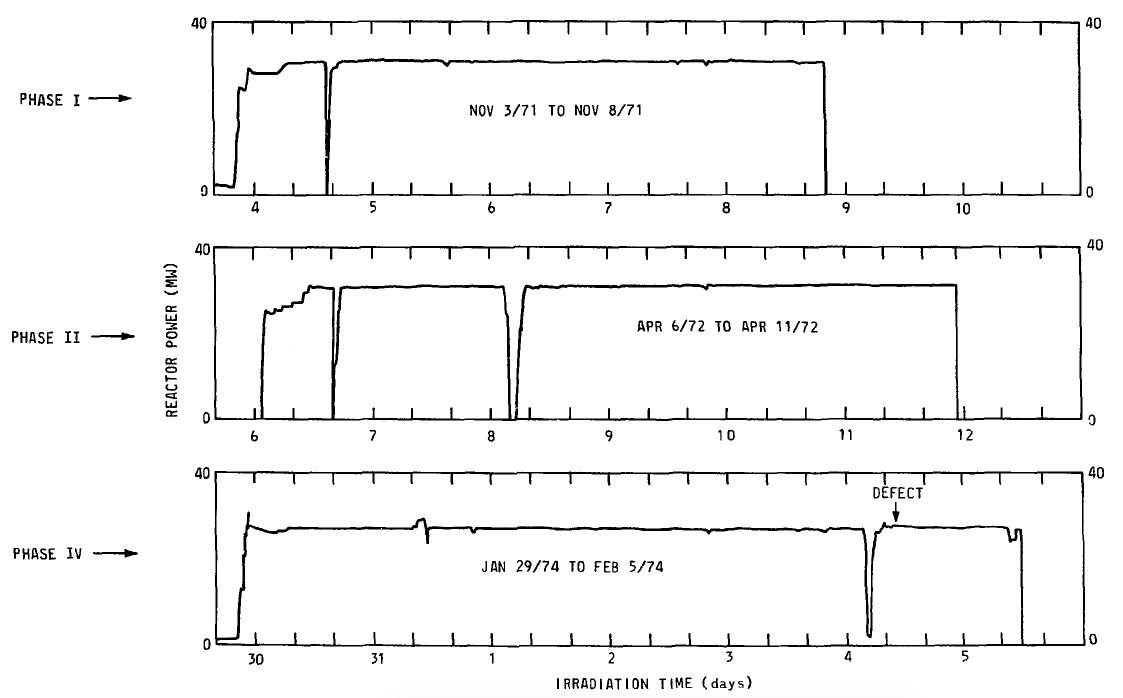
\includegraphics[width=\linewidth]{images/fueltests.png}
\caption[Power ramping test data for the different phases of the Chalk River Nuclear Lab experiment.]{Power ramping test data for the different phases of the Chalk River Nuclear Lab experiment. Taken from \cite{MacDonald1979}.}
\label{figure:fueltests}
\end{figure}
\end{landscape}

As discussed earlier, iodine is one of the most prevalent fission products and it is known to corrode zirconium metal. The exact mechanism by which this occurs in fuel pins is not yet known, though a combination of radiolysis, I$_{2}$ diffusion and chemical attack (I-SCC) are most likely. The most commonly proposed mechanism is illustrated in Figure \ref{figure:vanarkel}. In the first step, iodine and caesium are produced through fission of the fuel and diffuse towards the outer surface of the fuel pellet. A thin film of CsI is deposited on the outer surface of the fuel pellet and subsequently decomposes via radiolysis, liberating iodine in vapour form. This iodine vapour then diffuses towards a crack site in the cladding and reacts with Zr to produce ZrI$_{4}$. The ZrI$_{4}$ then breaks away from the metal due to the high surface energies, causing pitting and progressing the crack tip further into the metal.

\begin{figure}[ht]
\centering
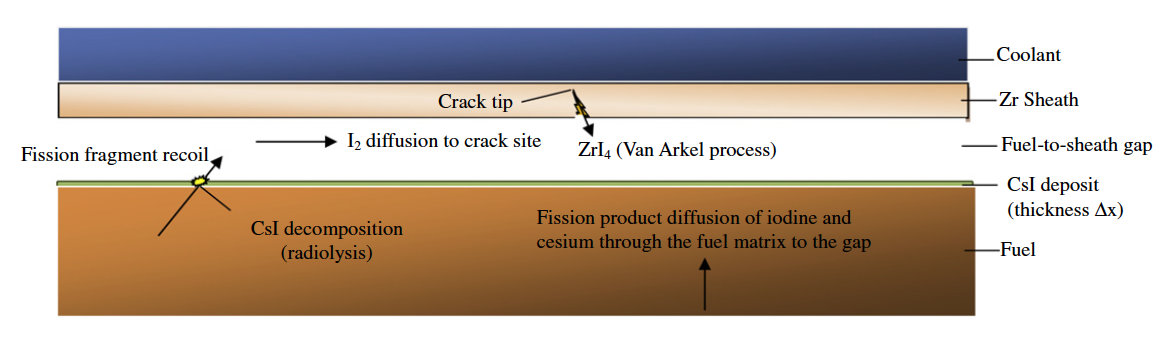
\includegraphics[width=\linewidth]{images/vanarkel.png}
\caption[Schematic of a proposed I-SCC process for cladding crack penetration.]{Schematic of a proposed I-SCC process for cladding crack penetration. Taken from \cite{Lewis2011}.}
\label{figure:vanarkel}
\end{figure}

The amount of free iodine available in the fuel pin is dependent on many different factors (e.g. temperature, pressure, power history, axial location in fuel pin, diffusion rate through fuel), making it difficult to measure. Thermodynamic calculations performed by Konashi \emph{et al}. estimate the equilibrium partial pressure of iodine in the fuel-cladding gap to be as low as 10$^{-17}$ atm when there is no radiolysis of CsI, and up to 10$^{-8}$ atm with the effect of CsI radiolysis included \cite{Konashi1983}. For comparison, mandrel tests of irradiated Zr claddings at 350 $^{\circ}$C show that susceptibility to I-SCC is reduced when the iodine partial pressure is below 60 Pa (approximately 6$\times 10^{-4}$ atm) \cite{anghel2010experimental}. While these calculated values of the iodine pressure are too low to induce corrosion in Zr, they demonstrate that radiation will increase the partial pressure of iodine by several orders of magnitude. Increasing reactor power (e.g. during a ramp) will increase radiation flux and therefore dissociation of CsI, however, no figures are yet available which demonstrate a clear link between this contribution to the iodine pressure and PCI failures. 

It is important however, to consider the role of oxygen in the I-SCC process. Fuel pins do not regularly fail during normal operation, despite iodine being produced continuously from fission of the fuel. This is because the inner surface of the cladding is not pure Zr metal, but rather a protective oxide which provides an effective barrier against corrosive species such as iodine.

\section{Oxidation of zirconium}

The oxidation of zirconium to produce \zirconia\ occurs during manufacture of the fuel cladding when the Zr metal is exposed to oxygen in air. \zirconia\ is a ceramic with material properties that make it desirable in many industrial applications, including solid-oxide fuel cells \cite{radford1979zirconia}, refractory linings \cite{whittemore1952fused}, and nuclear waste storage \cite{wang2012ceramics}. However, in the context of nuclear fuel cladding, the most important function of \zirconia\ is the barrier it provides against the ingress of corrosive species. 

\zirconia\ grown thermally on Zr metal exists mainly in either the monoclinic or tetragonal phase \cite{Howard1988,teufer1962crystal}. We can expect the internal \zirconia\ layer of the cladding to be mostly monoclinic in early life, with the stress-stabilised tetragonal phase appearing near the oxide/metal interface due to cohesive strains resulting from the lattice mismatch. With increasing burnup however, it is expected that more tetragonal and possibly even the cubic phase of \zirconia\ forms due to vacancy formation and residual stresses in the lattice from radiation damage \cite{sickafus1999radiation}. Amorphisation due to radiation damage has also been observed in the cubic phase from Cs$^{+}$ implantation \cite{amorphization2000wang}. In this thesis however, while defect energies for the cubic phase are reported (see Figures \ref{isolated_defects}, \ref{table:bound_defects}, \ref{figure:cubicinter}), we focus our analysis on monoclinic and tetragonal \zirconia\ phases, partly due to difficulties predicting the behaviour of the pure high-temperature cubic phase using energies calculated from a static energy technique. 

\subsection{Oxide growth mechanism}

An oxide layer will typically form on the surface of zirconium metal even at very low oxygen partial pressures \cite{causey2005review}. The oxidation process is mainly driven by the ingress of oxygen ions. Initially, the oxide is highly protective, growing slowly into the metal until it reaches a thickness of approximately 2-3 $\mu$m \cite{garzarolli1991oxide, dawson1968kinetics}, after which the oxide growth mechanism enters a `post-transition' stage where the oxidation kinetics follow a cubic-rate law  \cite{porte1960oxidation}. At low temperatures relative to the melting point or high pressures, and after reaching a critical thickness (called the transition point), parts of the initial oxide will fail and the oxidation rate will increase again. This process is illustrated in Figure \ref{figure:oxide_weight_gain}. 

\begin{figure}[ht]
\centering
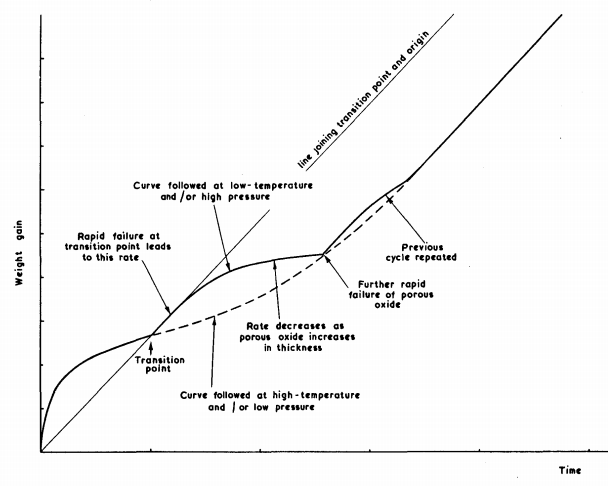
\includegraphics[height=10.5cm]{images/zro2_oxide_weight_gain.png}
\caption[Diagrammatic representation of the cyclical oxidation behaviour of \zirconia .]{Diagrammatic representation of the cyclical oxidation behaviour of \zirconia . Taken from \cite{cox1963some}.}
\label{figure:oxide_weight_gain}
\end{figure}

\subsection{Oxygen solubility of zirconium}

Looking at the Zr-O binary phase diagram in Figure \ref{figure:binary_phase_diagram}, oxygen is soluble in zirconium up to 29\% of total molar mass when below 400 $^{\circ}$C, the operating temperature region of a typical PWR (330 \textdegree C at the outer surface of the cladding). Solubility increases slightly up to 35\% of total molar mass as temperature is increased to the liquidus line at 2065 $^{\circ}$C. This is important to note because in the literature, it is assumed that there is pure Zr metal immediately beneath the \zirconia\ layer \cite{rossi2015first}, which is an assumption that will underestimate the extent to which repassivation occurs when the oxide layer is breached, and disregards the effect of the thin ZrO interface that can precede the metal. The molar mass of oxygen required to grow more oxide near the interface will therefore be at least 37\% lower than expected when using this assumption.

The presence of oxygen in the Zr metal will also have an effect on thermodynamic calculations of extrinsic defect formation. Atoms such as Te and I will have to compete with O atoms (and to some extent, self-interstitial Zr atoms) for interstitial sites in the metal. This increases the energy barrier to diffusion because of the lower availability of sites. An energy input is required to remove O or Zr atoms occupying these sites, making them a less favourable diffusion path.


\begin{figure}[ht]
\centering
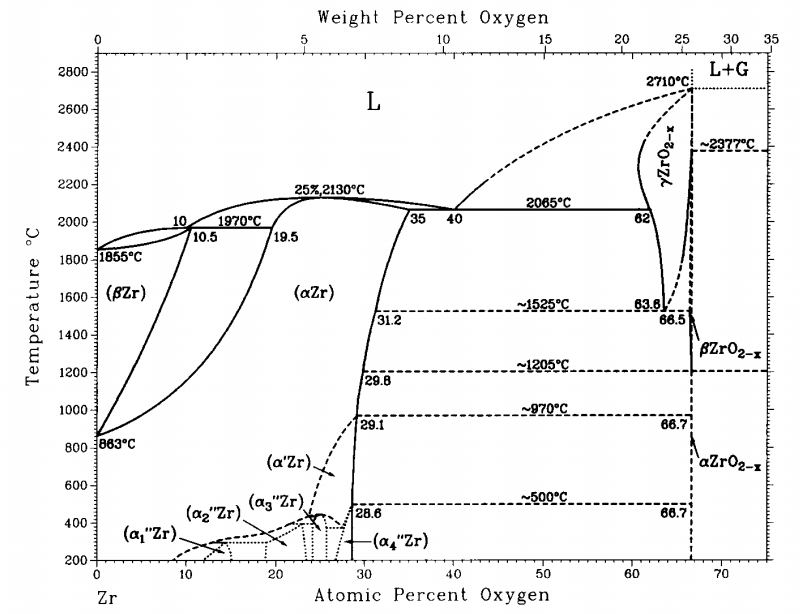
\includegraphics[width=14cm]{images/zro2_binary_phase.png}
\caption[Binary phase diagram of the Zr and O$_{2}$ system.]{Binary phase diagram of the Zr and O$_{2}$ system. Taken from \cite{Abriata1986}.}
\label{figure:binary_phase_diagram}
\end{figure}

\subsection{Outer oxide vs inner oxide} \label{section:outervsinner}

As mentioned previously, the cladding of an LWR fuel pin develops an oxide on both the inner and outer surfaces due to exposure to oxygen in air during manufacture. Both the outer and inner oxide layers provide protection against corrosion, though the corrosive environment is different. 

The outer oxide layer is in contact with the coolant which is mostly light water with some additional dissolved species such as boron and hydrogen to control reactivity and pH. Figure \ref{figure:outer_oxide} shows a section of the cladding with the outer oxide visible. This layer is mostly monoclinic \zirconia\ with small (nano) grains of tetragonal \zirconia\ distributed uniformly throughout. These grains of tetragonal \zirconia\ are autostabilised during growth of the oxide because of the large volume expansion associated with oxidation (Zr has a Pilling-Bedworth ratio of 1.57). Of course, transmission electron microscope (TEM) foils under examination are always stress-relieved, whereas the oxide in reactor conditions will be under 1-2 GPa of residual stress due to the growth of the oxide (see § \ref{section:tet_stress_stabilisation}).

\begin{figure}[ht]
\centering
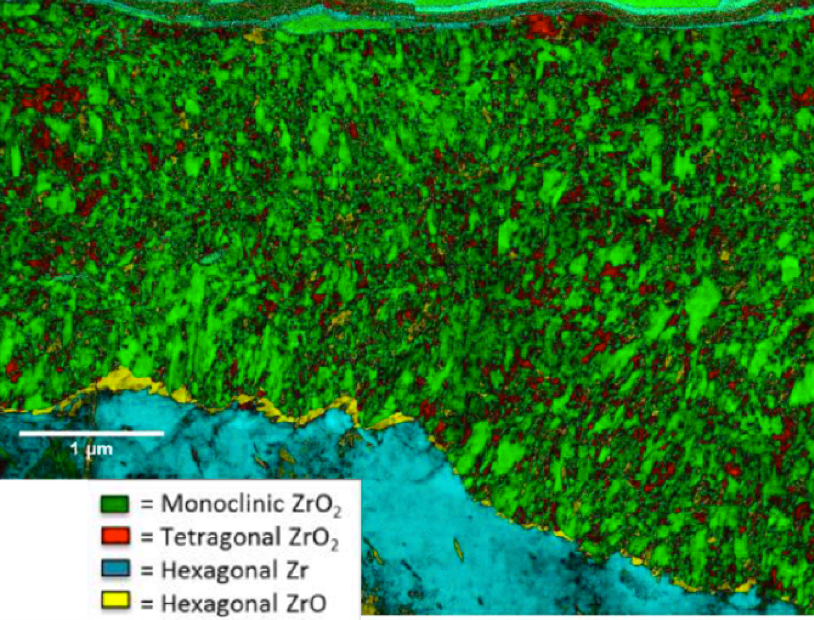
\includegraphics[height=10.5cm]{images/outer_oxide.png}
\caption[Scanning transmission electron microscrope (STEM) image of the outer oxide layer formed in an autoclave under simulated PWR water conditions showing the prevalence of different \zirconia\ phases.]{Scanning transmission electron microscrope (STEM) image of the outer oxide layer formed in an autoclave under simulated PWR water conditions showing the prevalence of different \zirconia\ phases. Taken from \cite{Hu2016}.}
\label{figure:outer_oxide}
\end{figure}

The internal oxide layer is much more challenging to examine due to the need to prepare samples in hot cells. This layer is typically very brittle due to radiation damage and implantation of fission products. At a high enough burnup, the \zirconia\ layer makes contact with the UO$_{2}$ fuel and will also bond together. Figure \ref{figure:inner_oxide} shows a section of the cladding with the inner oxide layer bonded to the pellet. The crystal structure of the \zirconia\ in this layer is debated. Some studies report no monoclinic phase in high burnup fuels, with cubic phase \zirconia\ throughout most of the layer and an amorphous phase nearer the pellet side \cite{Nogita1997}, while other studies report mostly tetragonal phase in this layer \cite{ciszak2017etude, gibert1998influence}. 
%After removal from the reactor and the subsequent cooling period, the inner oxide

\begin{figure}[ht]
\centering
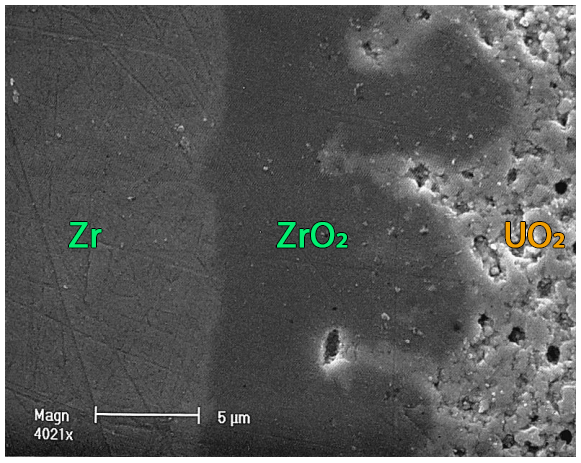
\includegraphics[height=10.5cm]{images/pci_bondinglayer.png}
\caption[High resolution scanning electron microscrope (SEM) image of the bonding layer between a PWR UO$_{2}$ fuel pellet and Zr cladding in a fuel pin at an approximate burnup of 60 GWd/tU.]{High resolution SEM image of the bonding layer between a PWR UO$_{2}$ fuel pellet and Zr cladding in a fuel pin at an approximate burnup of 60 GWd/tU. Taken from \cite{Lozano1998}.}
\label{figure:inner_oxide}
\end{figure}

Figure \ref{figure:bonding_layer_composition} shows the composition of the inner oxide of a high burnup fuel pin. The fission product (Ba, Mo, Nd) content is highest at the beginning of the \zirconia\ layer and decreases almost linearly with distance towards the Zr metal. This is due to fission product implantation rather than diffusion as these are highly immobile atoms. % can you use the weight composition and fission yields to estimate what percentage of iodine implantation will be?

\begin{figure}[ht!]
\centering
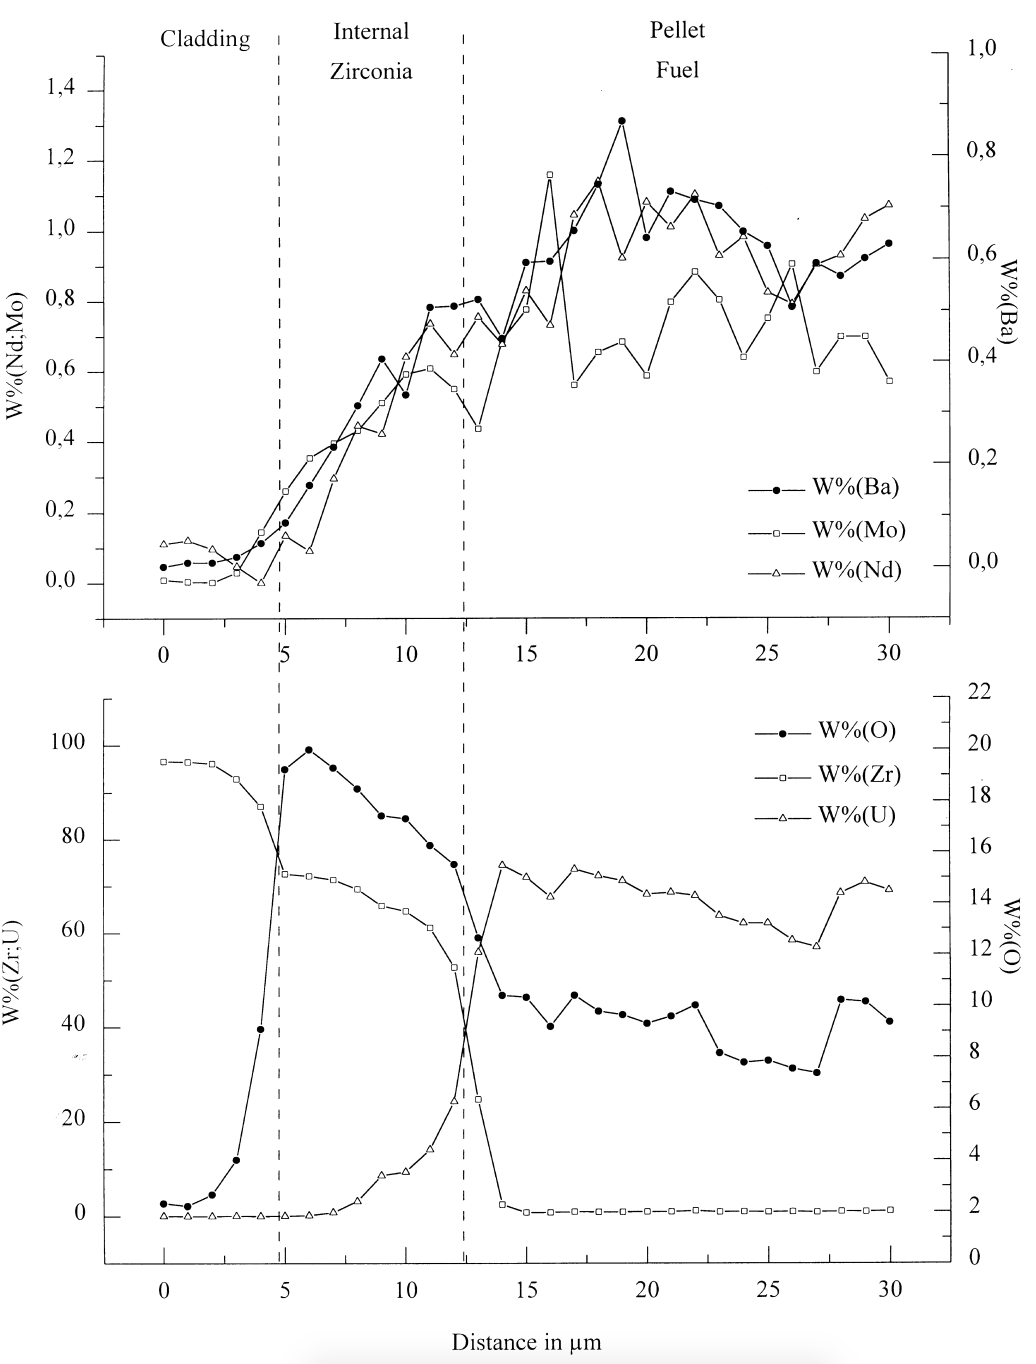
\includegraphics[width=14cm]{images/bonding_layer_composition.png}
\caption[Elemental composition of the bonded UO$_{2}$/ZrO$_{2}$ layer from a PWR UO$_{2}$ fuel pellet with a burnup of 61 GWd/tU.]{Elemental composition of the bonded UO$_{2}$/ZrO$_{2}$ layer from a PWR UO$_{2}$ fuel pellet with a burnup of 61 GWd/tU. Taken from \cite{Lozano1998}.}
\label{figure:bonding_layer_composition}
\end{figure}


\subsection{Sources of oxygen}

The internal oxide layer is present before fuel claddings are pressurised with helium gas and sealed. This is from the normal oxidation of Zr in air, where the oxygen pressure is 0.21 atm. After capping of the fuel rods, the only other available oxygen is from the UO$_{2}$ fuel pellets.

Uranium oxides have a wide range of non-stoichiometric compositions, with U/O ratios ranging from 1.67 to 2.24 in solid UO$_{2 \pm x}$, as shown in Figure \ref{figure:U_O_phase_diagram}. The oxide form U$_{3}$O$_{8-y}$ also exists and is more kinetically and thermodynamically stable than UO$_{2}$, but has lower density, making it less suitable for use as a fuel form. The different stoichiometries have different equilibrium O$_{2}$ pressures at constant temperature, allowing some level of tweaking the internal cladding environment depending on whether more or less oxygen is desired. 

Oxygen and oxygen precursors may also be produced directly from fission of U$_{235}$, but this contribution is insignificant compared to changing the stoichiometry of the fuel pellet. Indeed, liberation of oxygen from UO$_{2 \pm x}$ due to fission (which is also a function of the fuel's stoichiometry) is a more significant contributor to the oxygen pressure than direct production via fission.

\begin{figure}[ht]
\centering
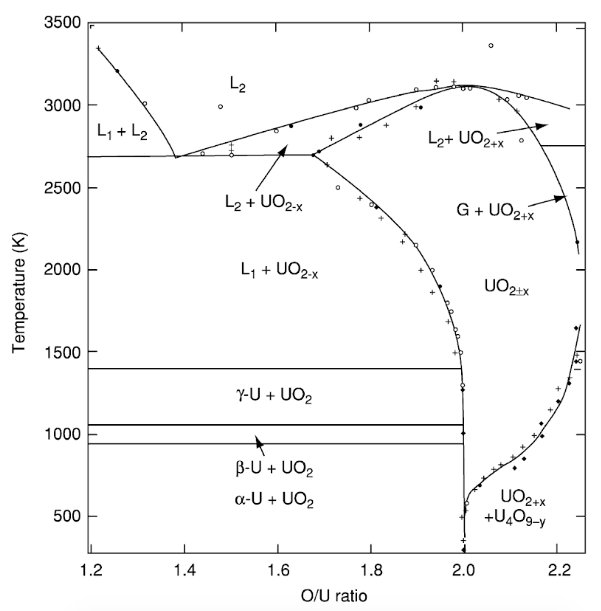
\includegraphics[height=12cm]{images/UO_phase_diagram.png}
\caption[Partial U-O temperature phase diagram between O/U ratios of 1.2 and 2.25.]{Partial U-O temperature phase diagram between O/U ratios of 1.2 and 2.25. Figure taken from \cite{katz2007chemistry}, with phase boundaries from \cite{rand1978thermodynamic, chevalier2002progress, gueneau2002thermodynamic}.}
\label{figure:U_O_phase_diagram}
\end{figure}


\section{Atomistic Simulation}

Conducting experiments on nuclear materials is a difficult undertaking. Handling irradiated materials is an expensive process, and materials such as uranium are highly controlled (though they are relatively benign before irradiation compared to many typical chemical laboratory materials and solvents). Furthermore, experiments which require samples to be irradiated must be left to cool-down (due to material activation) for up to a year before they can be analysed in a specialised lab \cite{efthymiopoulos2011hiradmat}. This makes it difficult to study many material phenomena, especially if they are time-dependent. In-situ reactor experiments are also problematic, requiring sensor equipment to be ruggedised for high radiation environments as well as obtaining special permission from a reactor operator (and the paperwork that entails) to conduct  such a test. Any errors in the experimental procedure or problems with samples are not revealed until months later when material analysis is performed. The risks and costs make it such that experimental work is mostly restricted to the largest labs and the few researchers with enough funding to support it.



\subsection{Classical approach - molecular dynamics}

Molecular dynamics (MD) uses classical mechanics as the basis for calculations. These types of simulations typically use pair potentials (though many-bodied potentials are also used). These are mathematical functions which effectively describe the energy of interaction between two particles. Pair potentials are created by fitting functions to several parameters from empirical data, such as equilibrium bond lengths, thermal properties or even values from quantum mechanical calculations. The simple form of pair potentials allows MD simulations to scale up to billions of atoms, corresponding to a length scale of approximately 0.1 $\mu$m. 

In the literature, many molecular dynamics studies of \zirconia\ exist. However, these studies typically focus on dopant-stabilised zirconias (i.e. cubic ones as empirical potentials don't capture monoclinic or tetragonal phases and their transitions accurately). The large system sizes possible in molecular dynamics simulations are often necessary for examining properties such as ion diffusion, thermal conductivity or melting points \cite{Davis2010}. Studying fission products in \zirconia\ however, requires potentials which can accurately model interactions of atoms such as Zr, O, and I in the solid phase. A good potential for such a system has not yet been published and so a quantum mechanical study of the \zirconia\ system is the focus of this thesis. The work herein may then be used in the future development of such potentials.

%These relatively large system sizes make MD a useful tool for studying a range of materials phenomena which are difficult to model at smaller scales, such as dislocations and long-range diffusion. 

%Add a figure here showing lennard jones. Also show the basic equations
%These are mainly pair potentials (although many-bodied potentials are also used) which are some combination of a short-range repulsion term (Pauli exclusion, nuclear repulsion if van der waals is taken into account) and a long range Coulombic attraction term

\subsection{Quantum mechanical approach - DFT}

Another method for modelling materials at the atomic scale is to use a quantum mechanical approach. In this thesis, the framework of density functional theory (DFT) is used throughout for quantum mechanical calculations (see § \ref{section:dft}). These techniques use a more fundamental approach than molecular dynamics, and are sometimes referred to as \emph{ab initio} methods (although several empirical approximations are often used in DFT). The CASTEP 8.0 software package was used for all DFT calculations \cite{Clark2005}.

System sizes are far more constrained when using DFT. The equations being solved scale combinatorially with the number of electrons and ions in the system, quickly becoming intractable even for simple molecules with a few atoms before applying DFT methods. There are several ways to significantly reduce the computational complexity without sacrificing too much accuracy (e.g. the pseudopotential method, periodic boundaries, cell constraints and symmetry). This allows system sizes on the order of hundreds of atoms to be studied, corresponding to a length scale of approximately 1 nm. While this length scale is much smaller than what can be achieved using MD, the use of a more fundamental parameter (electron density) in calculations provides a stronger scientific basis when material properties are derived from DFT models. Additionally, DFT allows electronic properties such as electron orbital occupancy and band gaps to be studied.

In the literature, DFT studies of \zirconia\ are predominantly focused on the dopant-stabilised cubic phase because of its use in fuel cells and medical applications \cite{orera1990intrinsic,jiang2011first}, with few studies on the undoped system \cite{mackrodt1986theoretical,aarhammar2009energetics}. Pure oxide studies also tend to focus on only one of the three common phase, typically the monoclinic \cite{zheng2007first,foster2002modelling,foster2001structure} and tetragonal phases \cite{Gionco2013, Eichler2004, Zhang2014}. Two notable studies have looked at all three phases. The first focused on the electronic structure and optical properties of \zirconia\ \cite{French1994}, while the second examined the structural properties and band structure of \zirconia\ \cite{Kralik1998}. Both studies utilised the LDA exchange-correlation functional. This functional has since been improved upon (see § \ref{section:kohnsham}), improving the accuracy of more recent models. However, it is always useful to compare to data from older studies. 

Lattice dielectric properties in the three phases have been calculated using DFT \cite{Zhao2002a}, and these have been used in this thesis to predict energies and defect equilibria. Various data from these studies have been used either for comparison or to aid in new calculations which have then been published.

\subsection{Band gap}

Conductors and insulators are two common ways to describe materials. While this binary characterisation may work as an approximation for many materials, in reality there is more of a continuum between these two states (e.g. semiconductors), and at the heart of this lies the band gap.

It is known that for ions, electron energy levels are quantised, restricting the range of possible electron energies to discrete quantities. More specifically, electrons can only occupy unique quantum states, defined by parameters such as quantum spin and angular momentum. In a crystal, where there are large numbers of electrons and many possible configurations of them, we refer to energy \emph{bands} which are comprised of many quantised energies. There are sometimes gaps between energy bands in crystals (illustrated in Figure \ref{figure:band_gap}) corresponding to energy levels that cannot be occupied, meaning that if electrons were to be added at the lowest energy levels one by one, there would occasionally be relatively large jumps in energy as an electron is forced to enter a higher energy band. 

\begin{figure}[ht]
\centering
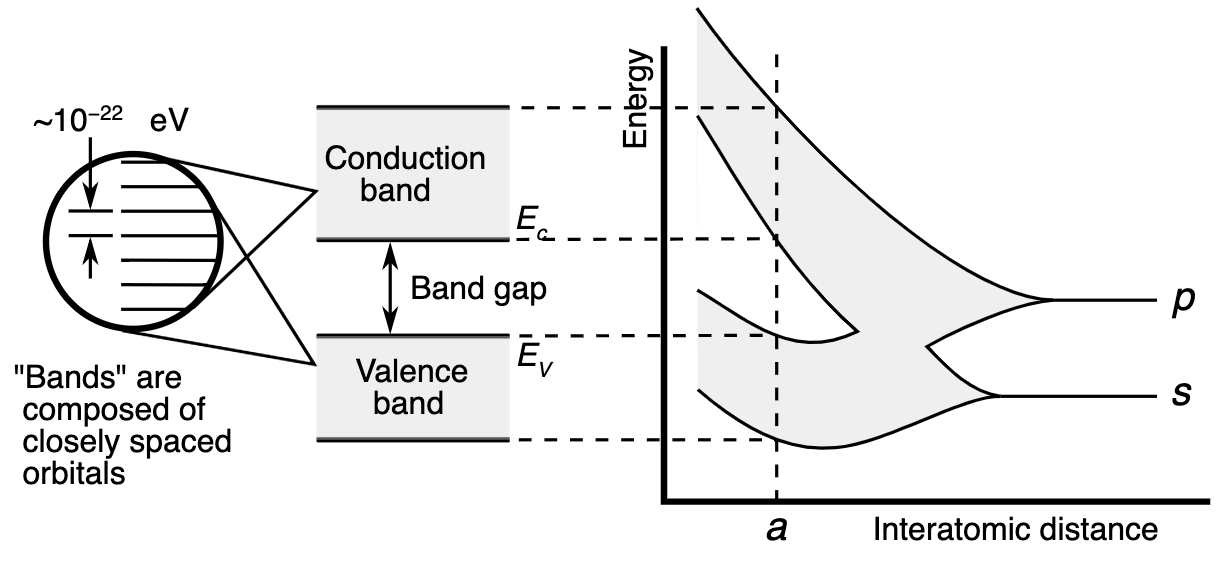
\includegraphics[width=\linewidth]{images/band_gap.png}
\caption[Illustration of the band gap in diamond as a function of interatomic spacing.]{Illustration of the band gap in diamond as a function of interatomic spacing. Taken from \cite{Chetvorno2017}.}
\label{figure:band_gap}
\end{figure}

Two energy bands, the \emph{valence band} and \emph{conduction band}, help determine a material's metallic or non-metallic character. The valence band contains energy levels occupied by the valence electrons (at absolute zero), while the conduction band contains energy levels which are high enough that electrons may freely move throughout the crystal. In metals, the valence and conduction bands have some amount of overlap, meaning that once the valence band is full, the highest occupied electron energy states are within the conduction band and so the material acts as a conductor. Materials like \zirconia , however, have large energy gaps between the valence and conduction bands, known as the band gap. These materials are called \emph{band insulators} (as opposed to \emph{Mott insulators} where there is no conventional band gap, but electron-electron interactions impede electron promotion to higher energies), because the band gap is an energy barrier preventing the valence electrons from moving freely around the crystal. 

In addition to the valence and conduction bands, a value for the electron chemical potential or Fermi level of the material is needed to determine how the energy bands are filled. If the Fermi level is exactly halfway between the valence band maximum (VBM) and the conduction band minimum (CBM), then the additional energy input required to promote an electron to the conduction band is half of the band gap. The Fermi level is strongly dependent on extrinsic defects and temperature. Extrinsic defects (called dopants) can be introduced to materials such as semiconductors in order to change the concentration of electronic defects (electrons and holes), while an increase in temperature will result in an increase in the Fermi level because of the larger amount of thermal energy available.

It is important to note that band gaps reported in DFT studies using classical LDA/GGA methods are significantly lower than those obtained experimentally. This is a known problem in DFT, and an exchange-correlation functional which reproduces correct band gap energies in semiconductors and insulators (without overfitting to experimental data) has not yet been discovered. The GW method, which uses a self-energy energy term in place of an exchange-correlation functional, allows more accurate\footnote{The GW approximation still has inaccuracies when modelling strongly correlated systems, but works well with $s$-$p$ systems.} estimates of the band gap than with DFT, but at a significantly higher computational expense. In many cases, the band gap from DFT calculations may be increased by appending an additional potential term, known as a +U parameter, to certain valence electron orbitals (discussed further in § \ref{subsection:plus_U}), or by using hybrid potentials which can incorporate the exact exchange energy.








%\section{Fission product empirical potential}
%
%In order to study the interaction of fission products with larger features in the cladding microstructure, such as dislocations and grain boundaries, it is necessary to develop empirical potentials for use in molecular dynamics simulations. Grain boundary transport is of particular interest, and this would require something on the order of 10$^{4}$ atoms to simulate to a reasonable degree of accuracy. This cannot be done using DFT currently due to the significant amount of computing resources required to run such a simulation. 
%
%The development of an iodine and xenon potential with \zirconia\ should be prioritised in order to run simulations to determine the migration of iodine within \zirconia, followed by the behaviour of xenon at the equilibrium iodine sites.
%
%\section{Grain boundary transport}
%
%Grain boundaries are interesting areas for studying species migration because diffusion towards the metal is expected to be more rapid through them than through bulk \zirconia .
%
%\section{Zr/ZrO/\zirconia\ interface study}
%
%The inner oxide is not a homogeneous structure, as described in § \ref{ch:crystallography}. Figure \ref{fig:zro_interface} clearly shows the existence of a ZrO phase up to 200 nm thick at the interface between \zirconia\ and Zr metal. The presence of ZrO and even oxygen-saturated Zr metal will have an effect on the thermodynamic equilibria of different fission products. An interface study can be conducted using DFT, to determine stresses at the interfaces of Zr and ZrO, and ZrO and \zirconia . Studying the aggregate effect of these interfaces on fission product behaviour may require larger molecular dynamics simulations, however. The crystal structure of the ZrO phase has been studied using both simulation and high-resolution electron microscopy, with two likely crystal structures being proposed \cite{Nicholls2015}. Further atomistic studies must be conducted to determine the stability of each crystal structure of ZrO when constrained by \zirconia\ and oxygen-saturated Zr metal interfaces.
%
%
%\begin{figure}[ht]
%    \centering
%    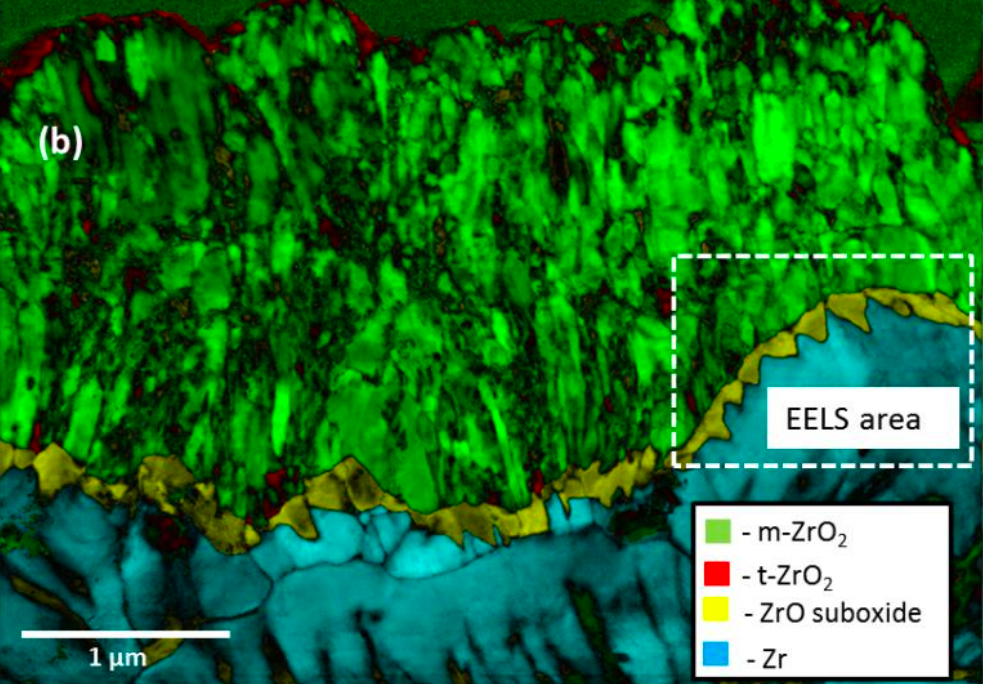
\includegraphics[height=9cm]{images/zro_interface.png}
%    \caption[STEM image of a Zr-1.0\%Nb sample oxidised in simulated PWR water at 360 C for 120 days.]{STEM image of a Zr-1.0\%Nb sample oxidised in simulated PWR water at 360 C for 120 days. Taken from \cite{inproceedings}.}
%    \label{fig:zro_interface}
%\end{figure} % Good
\chapter{Crystallography and Point Defects}

\label{ch:crystallography}

\section{\zirconia\ phases}
{\setstretch{1.4}
\zirconia\ exhibits three commonly reported polytypes in its binary phase diagram at ambient pressure. The temperature-pressure phase diagram of \zirconia\ as currently understood is shown in Figure \ref{figure:currentphasediagram}, with phase details in Table \ref{table:phases}. Each will now be described and contrasted.
}
%(see Figure \ref{figure:binary_phase_diagram})

\begin{figure}[ht] % Current phase diagram
\centering
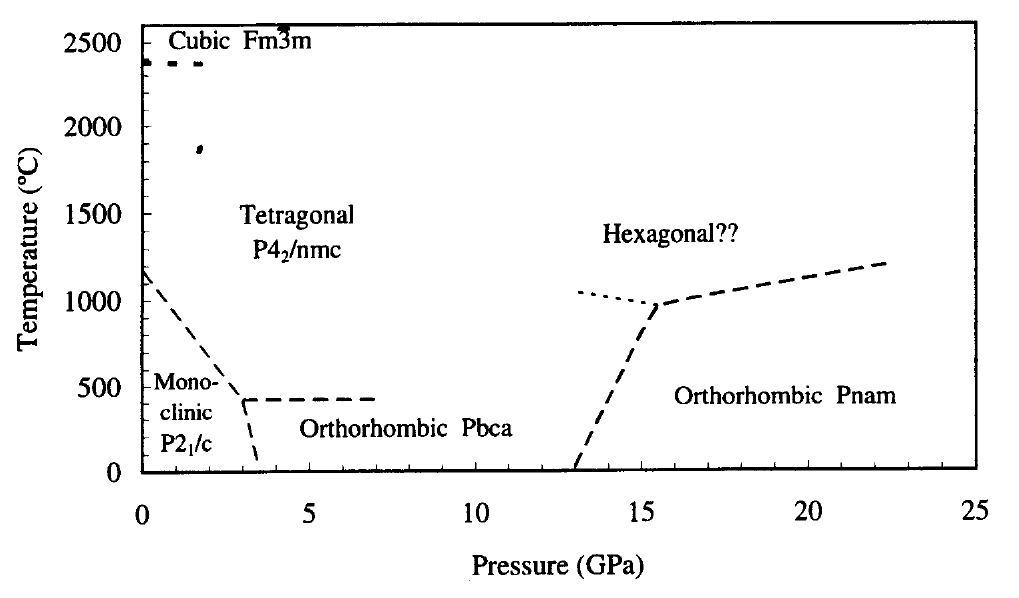
\includegraphics[height=7.7cm]{images/current_phase_diagram.png}
\caption[Temperature-pressure phase diagram of \zirconia .]{Temperature-pressure phase diagram of \zirconia . Taken from \cite{kisi1998crystal}.
\label{figure:currentphasediagram}}
\end{figure}

\begin{landscape}
\begin{center}
\begin{table}[ht]
\onehalfspacing
\centering
%\setlength\belowcaptionskip{0.2cm}
\caption[\zirconia\ phases and their details.]{\zirconia\ phases and their details. Adapted from \cite{kisi1998crystal}.}
\label{table:phases}
%\resizebox{\textwidth}{!}{%
\begin{tabular}{ccccccccccc}
\hline
\multirow{3}{*}{Phase} & \multirow{3}{*}{\begin{tabular}[c]{@{}c@{}}Stability\\ range\\ (K, GPa)\end{tabular}} & \multicolumn{4}{c}{\multirow{2}{*}{\begin{tabular}[c]{@{}c@{}}Cell parameters (\r{A})\\ (Extrapolated to room temperature)\end{tabular}}} & \multicolumn{4}{c}{\multirow{2}{*}{Atom positions}} & \multirow{3}{*}{\begin{tabular}[c]{@{}c@{}}Space\\ group\end{tabular}} \\
 &  & \multicolumn{4}{c}{} & \multicolumn{4}{c}{} &  \\ \cline{3-10}
 &  & $a$ & $b$ & $c$ & $\beta$ & Atom & $x$ & $y$ & $z$ &  \\ \hline
\multirow{2}{*}{Cubic \cite{terblanche1989thermal}} & \multirow{2}{*}{2377-2710 K} & \multirow{2}{*}{5.117} & \multirow{2}{*}{5.117} & \multirow{2}{*}{5.117} & \multirow{2}{*}{90} & Zr & 0 & 0 & 0 & \multirow{2}{*}{F$m\overline{3}m$} \\
 &  &  &  &  &  & O & 0.25 & 0.25 & 0.25 &  \\ \hline
\multirow{2}{*}{Tetragonal \cite{LANG1964}} & \multirow{2}{*}{1205-2377 K} & \multirow{2}{*}{5.074} & \multirow{2}{*}{5.074} & \multirow{2}{*}{5.188} & \multirow{2}{*}{90} & Zr & 0 & 0 & 0 & \multirow{2}{*}{P$4_{2}/nmc$} \\
 &  &  &  &  &  & O & 0.25 & 0.25 & 0.2044 &  \\ \hline
\multirow{3}{*}{Monoclinic \cite{Howard1988}} & \multirow{3}{*}{0-1205 K} & \multirow{3}{*}{5.1507} & \multirow{3}{*}{5.2028} & \multirow{3}{*}{5.3156} & \multirow{3}{*}{99.194} & Zr & 0.2754 & 0.0395 & 0.2083 & \multirow{3}{*}{P$2_{1}/c$} \\
 &  &  &  &  &  & O1 & 0.0700 & 0.3317 & 0.3477 &  \\
 &  &  &  &  &  & O2 & 0.4416 & 0.7569 & 0.4792 &  \\ \hline
\multirow{3}{*}{Ortho I \cite{ohtaka1990structural}} & \multirow{3}{*}{3.5-15 GPa} & \multirow{3}{*}{5.0431} & \multirow{3}{*}{5.2615} & \multirow{3}{*}{5.0910} & \multirow{3}{*}{90} & Zr & 0.2686 & 0.0332 & 0.2558 & \multirow{3}{*}{P$bca$} \\
 &  &  &  &  &  & O1 & 0.0822 & 0.3713 & 0.1310 &  \\
 &  &  &  &  &  & O2 & 0.5442 & 0.2447 & 0.0052 &  \\ \hline
\multirow{3}{*}{\begin{tabular}[c]{@{}c@{}}Ortho II \cite{Haines1995} \\ (cotunnite)\end{tabular}} & \multirow{3}{*}{\textgreater 15 GPa} & \multirow{3}{*}{5.593} & \multirow{3}{*}{6.484} & \multirow{3}{*}{3.333} & \multirow{3}{*}{90} & Zr & 0.256 & 0.110 & 0.25 & \multirow{3}{*}{P$nma$} \\
 &  &  &  &  &  & O1 & 0.356 & 0.422 & 0.25 &  \\
 &  &  &  &  &  & O2 & 0.022 & 0.331 & 0.75 &  \\ \hline
\multirow{3}{*}{Ortho (PSZ) \cite{kisi1989crystal}} & \multirow{3}{*}{0-500 K} & \multirow{3}{*}{5.068} & \multirow{3}{*}{5.260} & \multirow{3}{*}{5.077} & \multirow{3}{*}{90} & Zr & 0.267 & 0.030 & 0.250 & \multirow{3}{*}{P$bc2_{1}$} \\
 &  &  &  &  &  & O1 & 0.068 & 0.361 & 0.106 &  \\
 &  &  &  &  &  & O2 & 0.537 & 0.229 & 0 &  \\ \hline
\end{tabular}%
\end{table}
\end{center}
\end{landscape}

%Zirconia-based ceramics are used in a variety of technological and commercial applications, ranging from thermal barriercoatings on aircraft turbines to affordable diamond substitutes[167,168]. Recently, zirconia has received attention as an alternative dielectrics to silicon dioxide for memory and logic devices [169]. The versatility of zirconia originates entirely fromatomic or point defects in the crystal created by adding aliovalent oxides, e.g., MgO, La2O3, and Y2O3. The substitutionalcations or dopants that are charge balanced by the formation ofoxygen vacancies, and their mutual interactions, dramaticallyaffect the structural, thermal, mechanical, and electrical properties of modified or stabilized zirconia (SZ). These defects aresolely responsible for the high ionic conductivity of doped zirconia that underlies its use in oxygen sensors [170], and hightemperature fuel cells [171]. Zirconia is also used as a support material in heterogeneous catalysis [172].


\subsection{Monoclinic}

Below 1205 K at atmospheric pressure, \zirconia\ adopts a monoclinic Baddeleyite (P$2_{1}/c$) crystal structure. This is the ground state structure of \zirconia . In this phase, Zr ions have a sevenfold O coordination, down from eight in the higher temperature phases due to a single `broken bond'. A unit cell of monoclinic \zirconia\ is illustrated in Figure \ref{figure:coordination}. The dashed line (approximately 3.7\r{A} in length) shows the Zr-O bond which is broken when transitioning to monoclinic from the tetragonal phase. Zr-O bond lengths range from 2.05 to 2.31 \r{A}.

\begin{figure}[ht] % Mono coordination figure
\centering
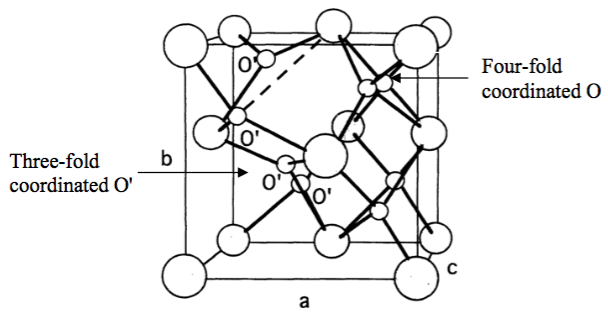
\includegraphics[height=7.5cm]{images/coordination.png}
\caption[A monoclinic zirconia unit cell indicating the two different oxygen bond coordinations. Small spheres represent oxygen ions while large spheres represent zirconium ions.]{A monoclinic zirconia unit cell indicating the two different oxygen bond coordinations. Small spheres represent oxygen ions while large spheres represent zirconium ions. Taken from \cite{Xia2010}.
\label{figure:coordination}}
\end{figure}

Monoclinic phase \zirconia\ also has two distinct oxygen ions in its primitive cell. To maintain the stoichiometry of 1:2 Zr to O, half of the oxygen ions exhibit threefold coordination with zirconium (in a planar configuration), while the other half have a fourfold coordination (tetrahedral configuration) with zirconium. Figure \ref{figure:monoschottky} shows the positions of these oxygen ions around a zirconium ion centre. The distortion from the oxygen rock salt sub-lattice can be seen, specifically in the case of the three coordinated oxygen ions. This is due to the zirconium ion being too small to hold 8 oxygen ions in an octahedral configuration, as in the fluorite crystal structure. As temperature is increased, so too are the interatomic distances. At the tetragonal temperature range, bonding between all 8 nearest neighbour oxygen and zirconium ions becomes energetically favourable and there is a transition to eightfold coordination.

\begin{figure}[ht] % Mono Zr centre
\centering
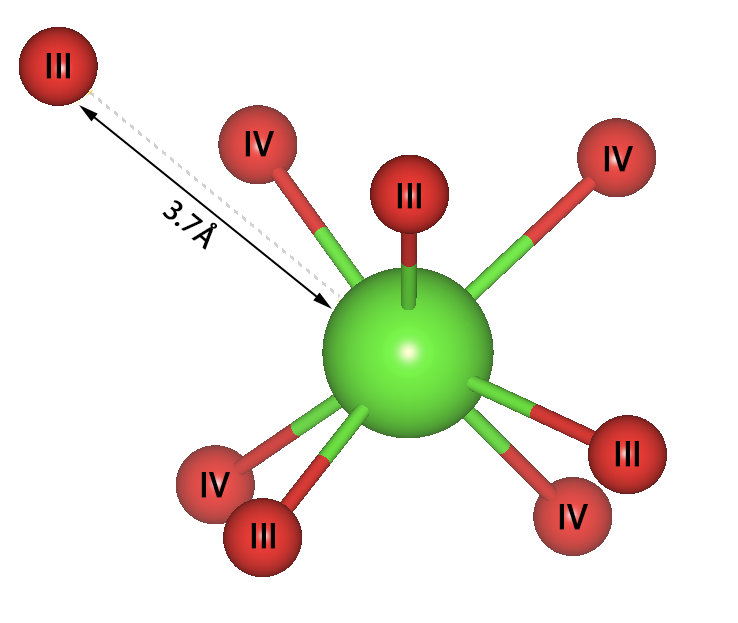
\includegraphics[height=8.5cm]{images/mono_zr_centre.png}
\caption{Zirconium centre unit cell in monoclinic \zirconia\ showing nearest oxygen atoms and their respective bond co-ordinations. Zirconium atoms are shown in green and oxygen atoms in red.}
\label{figure:monoschottky}
\end{figure}

The monoclinic-tetragonal phase transition occurs by a diffusionless martensitic transformation with a 9\textdegree\ shear \cite{Subbarao1974}. This is a fast transformation and is accompanied by a large volume change. Tetragonal phase \zirconia\ (density 6.10 g/cm$^{3}$) is around 4.6\% more dense than monoclinic \zirconia\ (density 5.83 g/cm$^{3}$) \cite{McCullough2002}, though the volume increase when cooling from tetragonal has been reported to be as high as 9\% \cite{Gupta1977}. This results in a kinetic barrier between the phases, and therefore the phase transition exhibits a hysteresis loop approximately 200 K wide when undergoing thermal cycling, as shown in Figure \ref{figure:hysteresis_monotet}.

\begin{figure}[ht] % Hysteresis
\centering
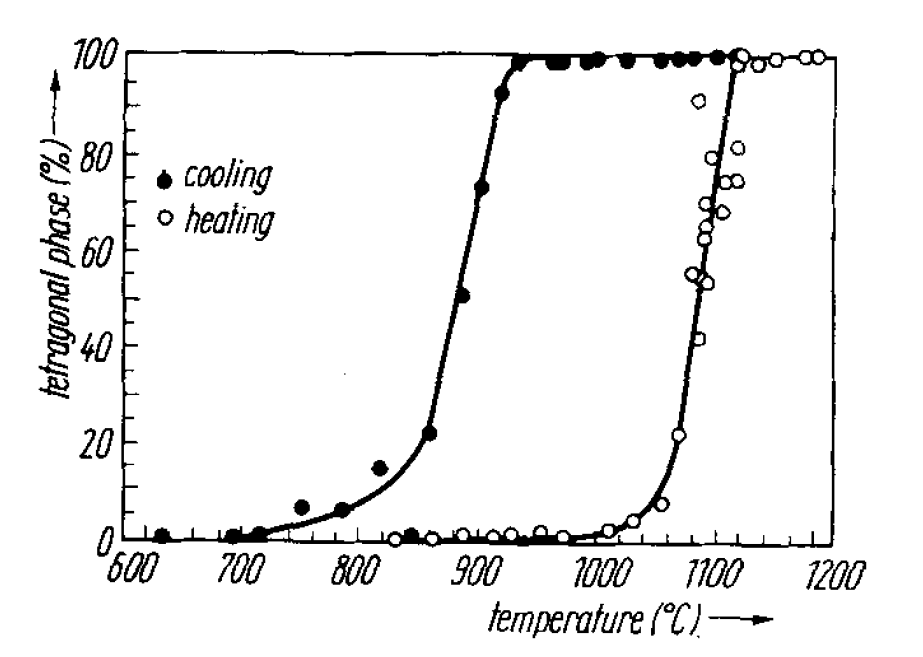
\includegraphics[width=12cm]{images/hysteresis_monotet.png}
\caption[Monoclinic-tetragonal phase transition in \zirconia\ as a function of temperature only.]{Monoclinic-tetragonal phase transition in \zirconia\ as a function of temperature only. Taken from \cite{WOLTEN1963}.}
\label{figure:hysteresis_monotet}
\end{figure}

%\begin{table}[ht]
%\centering
%\onehalfspacing
%\caption{\zirconia\ crystal structures and their stable temperatures at 1 atm \cite{Howard1988}.}
%\label{table:phases}
%\begin{tabular}{ccc}
%\hline
%{Crystal Structure} & {Space Group}    & {Temperature Range (K)} \\ \hline
%\multicolumn{1}{c}{Monoclinic} & \multicolumn{1}{c}{$P2_1/c$} & \multicolumn{1}{c}{$T$ \textless\ 1440}     \\
%\multicolumn{1}{c}{Tetragonal} & \multicolumn{1}{c}{$P4_2/nmc$} & \multicolumn{1}{c}{1440 \textless\ $T$ \textless\ 2640}        \\
%\multicolumn{1}{c}{Cubic} & \multicolumn{1}{c}{$Fm\overline{3}m$}     & \multicolumn{1}{c}{2640 \textless\ $T$ \textless\ 2950}      \\ \hline
%\end{tabular}
%\end{table}

\subsection{Tetragonal}

The tetragonal phase (space group P$4_{2}/nmc$) can be easily derived from the cubic phase by shifting alternating columns of oxygen ions slightly up or down the [001] direction. This change is so subtle that the two phases are almost identical when viewed in certain orientations. Figure \ref{figure:tetvscubic} shows a view of a tetragonal unit cell down the [110] direction alongside a [100] view of a cubic unit cell. Going from the cubic to the tetragonal phase, the oxygen ions can clearly be seen to deviate from their equilibrium sites in the cubic sublattice. This is consistent with the interpretation that the ionic radius of Zr is slightly too small to maintain the cubic fluorite structure, which is therefore only seen at high temperatures (where thermal fluctuations mean the effective ionic radius is larger) or when under high compressive stress (where interatomic spacings are smaller).

\begin{figure}[ht]
\centering
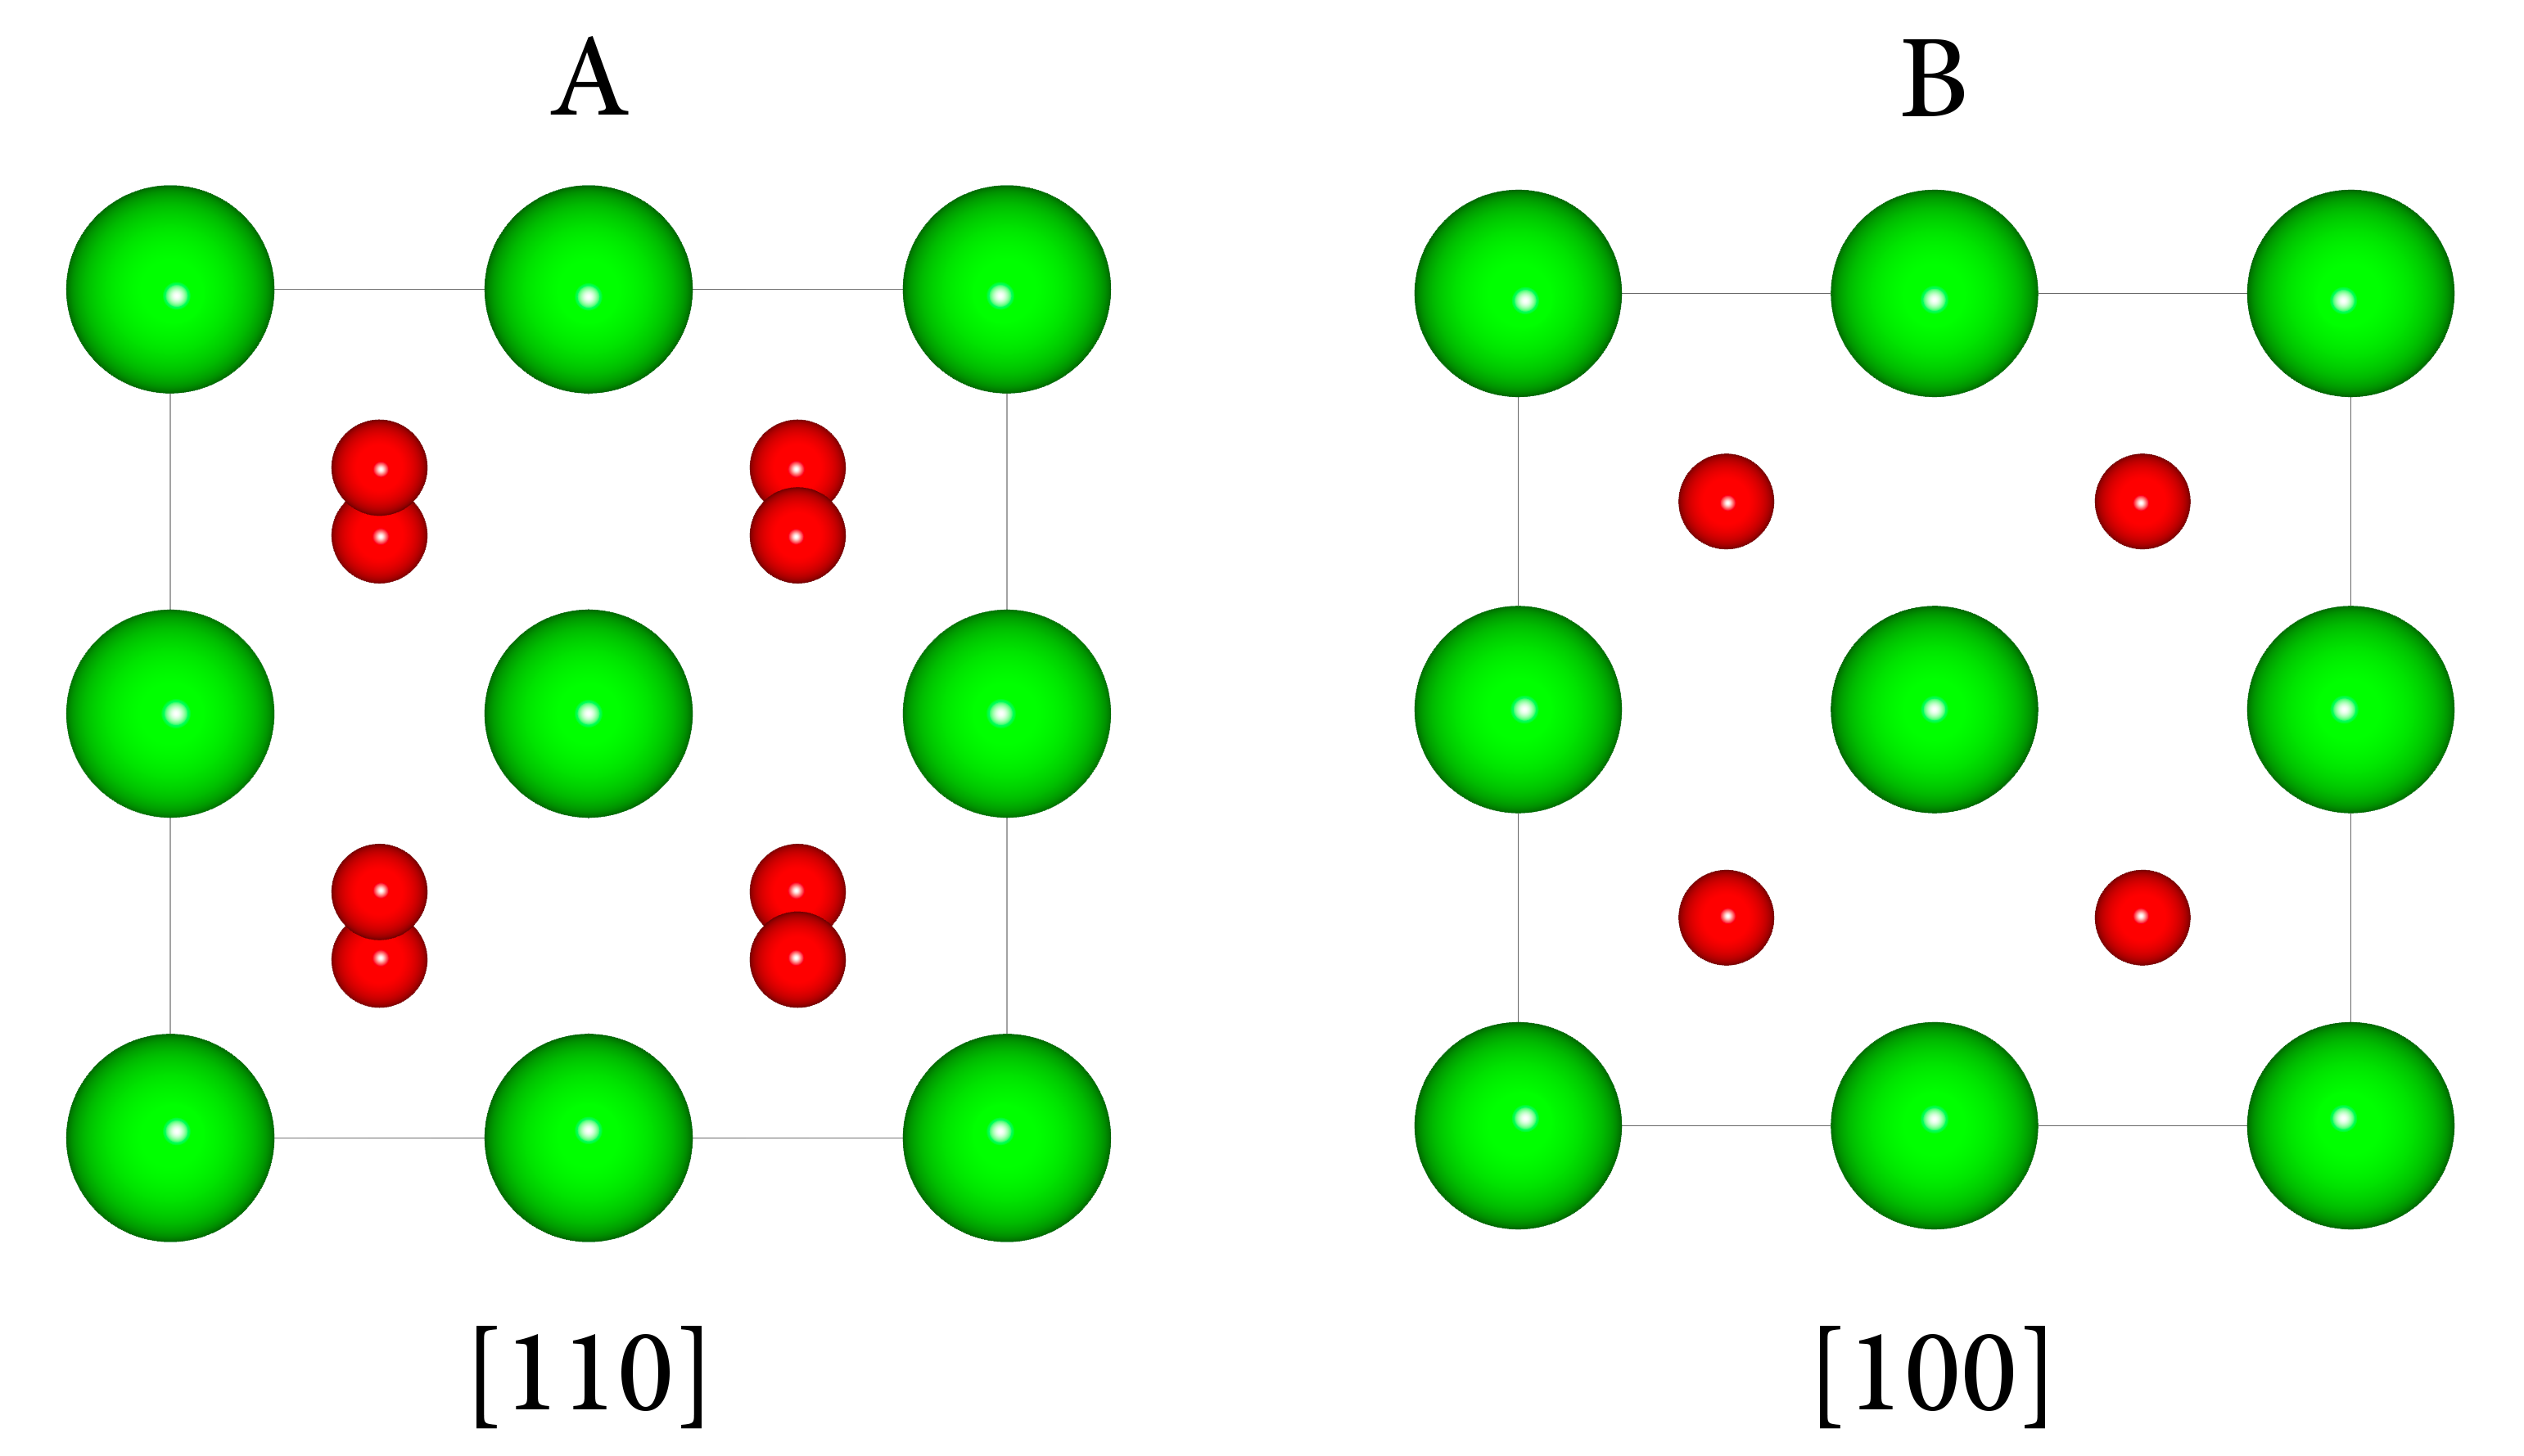
\includegraphics[width=14cm]{images/tet_vs_cubic.png}
\caption{\textbf{A}) Tetragonal \zirconia\ viewed along the [110] direction. \textbf{B}) Cubic \zirconia\ viewed along the [100] direction. Zirconium atoms are shown in green and oxygen atoms in red.}
\label{figure:tetvscubic}
\end{figure}

\subsubsection{Tetragonal phase stress stabilisation} \label{section:tet_stress_stabilisation}

The pressure-temperature phase diagram of \zirconia\ (Figure \ref{fig:phasediagram})\footnotemark\ shows how the monoclinic-tetragonal phase transition temperature is strongly dependent on pressure, with an almost linear reduction in transition temperature of 300 \textdegree C/GPa. The phase diagram also shows the extent of the hysteresis effect in the monoclinic-tetragonal transition. 

\footnotetext{Tetragonal I in this figure refers to the high temperature tetragonal phase of \zirconia\ with space group $P4_{2}/nmc$. Tetragonal II refers to the high pressure orthorhombic phase with space group $Pbca$. However, the authors indexed this phase on the basis of a tetragonal cell.}

%\begin{figure}[ht] 
%  \centering
%      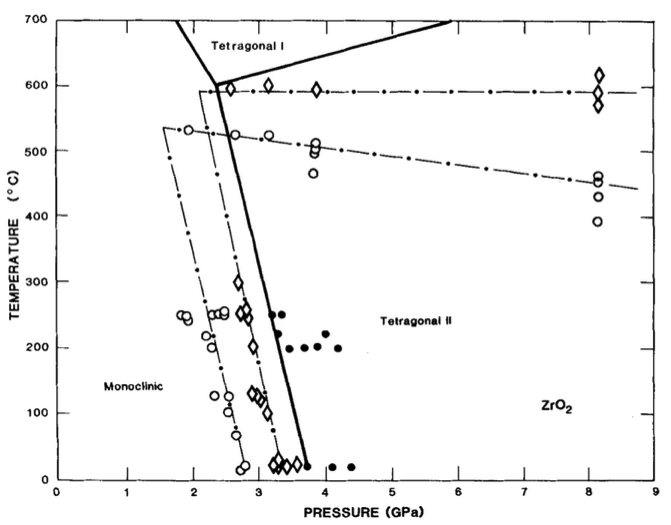
\includegraphics[width=13cm]{images/zirconiaphasediagram.png}
%  \caption[Pressure-temperature phase diagram for zirconia. Dash-dotted lines represent more recent data. Diamonds mark transition points during an increase in temperature of pressure, while open circles represent a decrease in pressure or temperature. Solid circles represent transition points for a fresh, single crystal sample.]{Pressure-temperature phase diagram for zirconia. Dash-dotted lines represent more recent data. Diamonds mark transition points during an increase in temperature of pressure, while open circles represent a decrease in pressure or temperature. Solid circles represent transition points for a fresh, single crystal sample. Taken from \cite{block1985pressure}.}
%\label{fig:phasediagram}
%\end{figure}
%

\begin{figure}[ht]
  \centering
      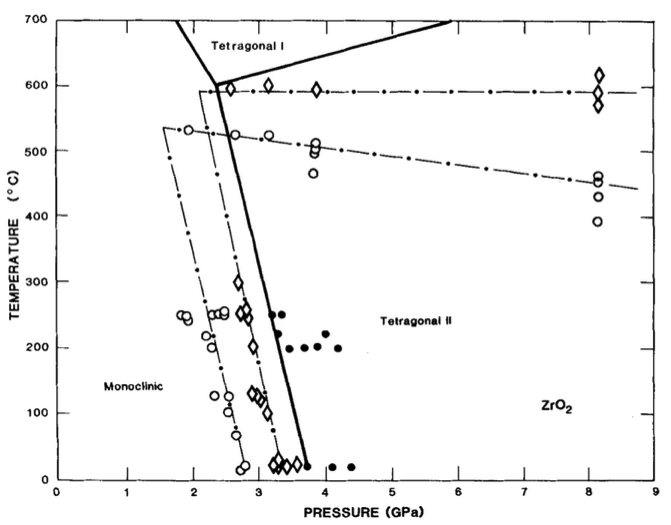
\includegraphics[width=13cm]{images/zirconiaphasediagram.png}
  \caption[Pressure-temperature phase diagram for zirconia. Dash-dotted lines represent more recent data. Diamonds mark transition points during an increase in temperature of pressure, while open circles represent a decrease in pressure or temperature. Solid circles represent transition points for a fresh, single crystal sample.]{Pressure-temperature phase diagram for zirconia. Dash-dotted lines represent more recent data. Diamonds mark transition points during an increase in temperature of pressure, while open circles represent a decrease in pressure or temperature. Solid circles represent transition points for a fresh, single crystal sample. Taken from \cite{block1985pressure}. \label{fig:phasediagram}}
\end{figure}


There is some degree of tetragonal phase autostabilisation during the oxidation process of zirconium. This is possible because of the resulting increase in volume when zirconium is oxidised. Zirconium has a Pilling-Bedworth ratio of 1.57, meaning that the oxide would occupy a volume 57\% larger than the metal if unconstrained \cite{cramer2003corrosion, Pilling1923}. In the case of zirconia, the oxide grows into the metal by transport of oxygen through the oxide layer to the metal/oxide interface, generating large compressive stresses of up to 2 GPa \cite{Petigny2000, garzarolli1991oxide}. This is an important contribution to the stabilisation of the tetragonal phase because of the strong dependence on pressure, though this contribution alone may not be sufficient at PWR operating temperatures.

Stabilisation of the tetragonal phase at low temperatures is also dependent on grain size, which can be controlled during the cladding manufacturing process since the oxide inherits the grain size of the zirconium metal grains. Pure \zirconia\ exhibits a strong relationship between grain size and phase stability, where the tetragonal phase is only stable when grown from metal grains below a critical size of approximately 30 nm \cite{barberis1995zirconia}. This can be explained by increased dislocation interaction in smaller grains due to limited room for dislocation glide, as per the Hall-Petch relationship \cite{hall1951deformation, petch1953cleavage}. Grains of tetragonal \zirconia\ larger than this critical size are therefore likely to have tetragonal-stabilising dopant ions incorporated in the lattice.

\subsection{Cubic}

Cubic \zirconia\ (unit cell shown in Figure \ref{fig:cubic_unitcell}) adopts the cubic fluorite (space group F$m\overline{3}m$) crystal structure, consisting of zirconium ions in a face-centred cubic configuration with a rock salt oxygen sub-lattice occupying the tetrahedral sites.

\begin{figure}[ht]
  \centering
      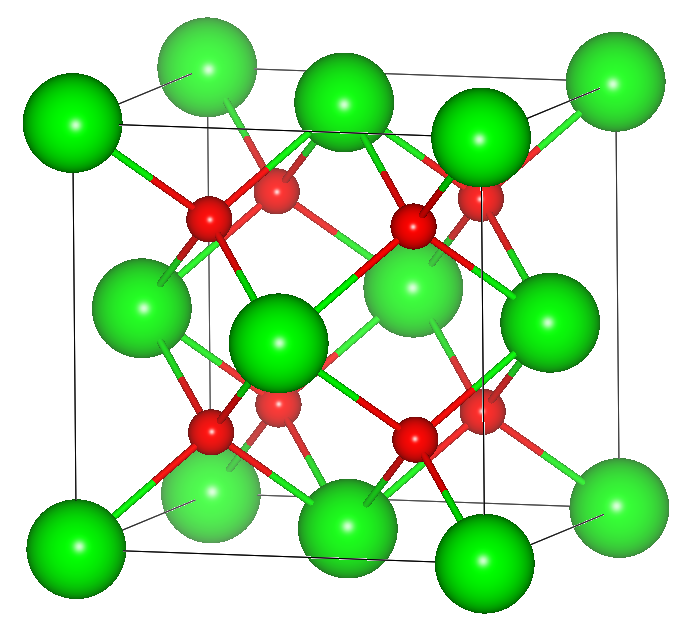
\includegraphics[height=7cm]{images/cubic_unitcell.png}
  \caption{Unit cell of cubic \zirconia . Zirconium atoms are shown in green and oxygen atoms shown in red.}
  \label{fig:cubic_unitcell}
\end{figure}

The lowest specific volume (i.e. highest density), as calculated from DFT geometry optimisations in this thesis, is exhibited by the cubic phase (11.13 \r{A}$^{3}$ion$^{-1}$) followed by the tetragonal phase (11.51 \r{A}$^{3}$ion$^{-1}$) and then the monoclinic phase (11.99 \r{A}$^{3}$ion$^{-1}$). This is due to it having the largest atomic packing factor, resulting in a mean Zr-O bond distance of 2.22 \r{A}, compared to 2.26 \r{A} in the tetragonal phase and 2.31 \r{A} in the monoclinic phase, as shown in Figure \ref{figure:zrobonddistance}. 

\begin{figure}[ht]
\begin{center}
\begin{tikzpicture}
	\begin{axis}
		[width=\linewidth*0.7, xlabel={Nearest neighbour Zr-O bond distance (\r{A})}, ylabel={Relative occurrence}, ymin=0, ymax=140, xmin=2.0, xmax=2.50, legend style={{draw=}, at={(0.95,0.95)}, anchor=north east, legend columns=1}]
		\addplot[no marks] table [x=zr_o_dist, y=monoclinic,]{dat/zr_o_bond_distances.dat}; \addlegendentry{Monoclinic};
        \addplot[no marks, dashed] table [x=zr_o_dist, y=tetragonal, ]{dat/zr_o_bond_distances.dat}; \addlegendentry{Tetragonal};
        \addplot[no marks, densely dotted] table [x=zr_o_dist, y=cubic,]{dat/zr_o_bond_distances.dat}; \addlegendentry{Cubic};
			\end{axis}
		\end{tikzpicture}
		\caption{Density plot of the nearest neighbour Zr-O bond distances in \zirconia\ for each crystal structure. Specific volumes from DFT calculations are 11.99 \r{A}$^{3}$ion$^{-1}$, 11.51 \r{A}$^{3}$ion$^{-1}$, and 11.13 \r{A}$^{3}$ion$^{-1}$ for monoclinic, tetragonal, and cubic phases respectively.}
		\label{figure:zrobonddistance}
	\end{center}
\end{figure}


%\textbf{Also due to the high temperature, the stability of the cubic phase in DFT calculations may be inaccurate. This is discussed further in Chapter 3.}


\subsection{Other phases}

Two orthorhombic phases have also been observed at high pressures in pure \zirconia\ \cite{howard1991crystal}. These structures are referred to as OI and OII, the latter of which is isostructural with cotunnite (PbCl$_{2}$). A third orthorhombic phase ($bc2_{1}$) has also been reported in partially stabilised zirconia (PSZ), but has not been found in pure zirconia \cite{kisi1998crystal}.

\subsubsection{Orthorhombic OI}

The OI phase, illustrated in Figure \ref{fig:orthorhombic_I}, maintains a 7 oxygen coordinated zirconium ion, as is the case in the monoclinic phase. This phase also exhibits two distinct oxygen atom sites like in the monoclinic phase, but being an orthorhombic phase, it does not exhibit a 9\textdegree\ shear in its unit cell like the monoclinic phase. While this phase is briefly stable at high compressive stresses (3.5 - 15 GPa), it appears to be an intermediate phase before collapse into the more familiar cotunnite structure at pressures greater than 15 GPa. In addition, the OI phase is only stable at temperatures below approximately 400 \textdegree C, transitioning to the tetragonal phase at higher temperatures. While PWRs operate at low enough temperatures for the OI phase to be stable, compressive stresses on the order of several GPa will not be present at any significant scale and thus this phase will not affect the oxide microstructure. 


\begin{figure}[ht]
  \centering
      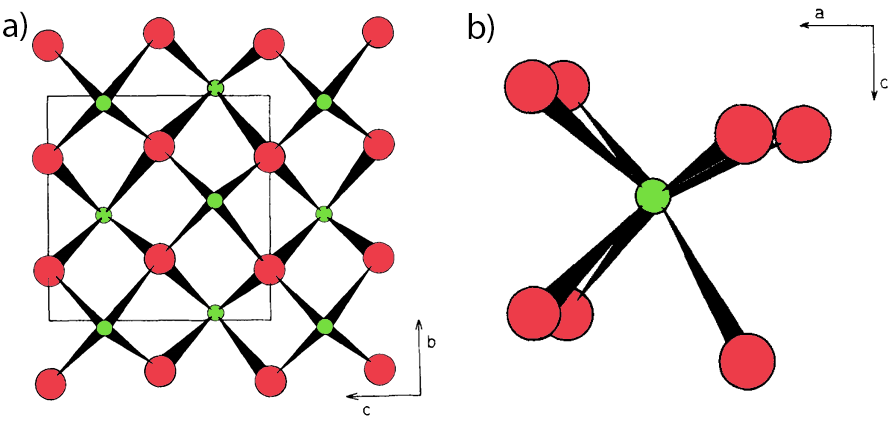
\includegraphics[width=\linewidth]{images/orthorhombic_I.png}
  \caption[Illustrations of the orthorhombic OI (P$bca$) crystal structure of \zirconia\ showing \textbf{a)} the unit cell viewed along the $a$ direction and \textbf{b)} the zirconium ion centre with 7 coordinated oxygen ions. Zirconium and oxygen ions are coloured green and red respectively.]{Illustrations of the orthorhombic OI (P$bca$) crystal structure of \zirconia\ showing \textbf{a)} the unit cell as seen from the $a$ direction and \textbf{b)} the zirconium ion centre with 7 coordinated oxygen ions. Zirconium and oxygen ions are coloured green and red respectively. Adapted from \cite{kisi1989crystal}.}
  \label{fig:orthorhombic_I}
\end{figure}


\subsubsection{Orthorhombic OII (cotunnite)}

The OII phase, illustrated in Figure \ref{fig:cotunnite_structure} maintains a 9 oxygen coordinated zirconium ion. This is due to the high stabilising pressure ($>$ 15 GPa) causing a reduction in the mean interatomic distance, so much so that the zirconium ion, which is typically too small to bond strongly to more than 7 oxygen atoms at standard conditions, can maintain the ninefold oxygen coordination. Such high hydrostatic pressures will not be present in a reactor environment even at the atomic scale, it is therefore not expected to find any OII phase present at any point during the cladding's operational lifetime.

\begin{figure}[ht]
  \centering
      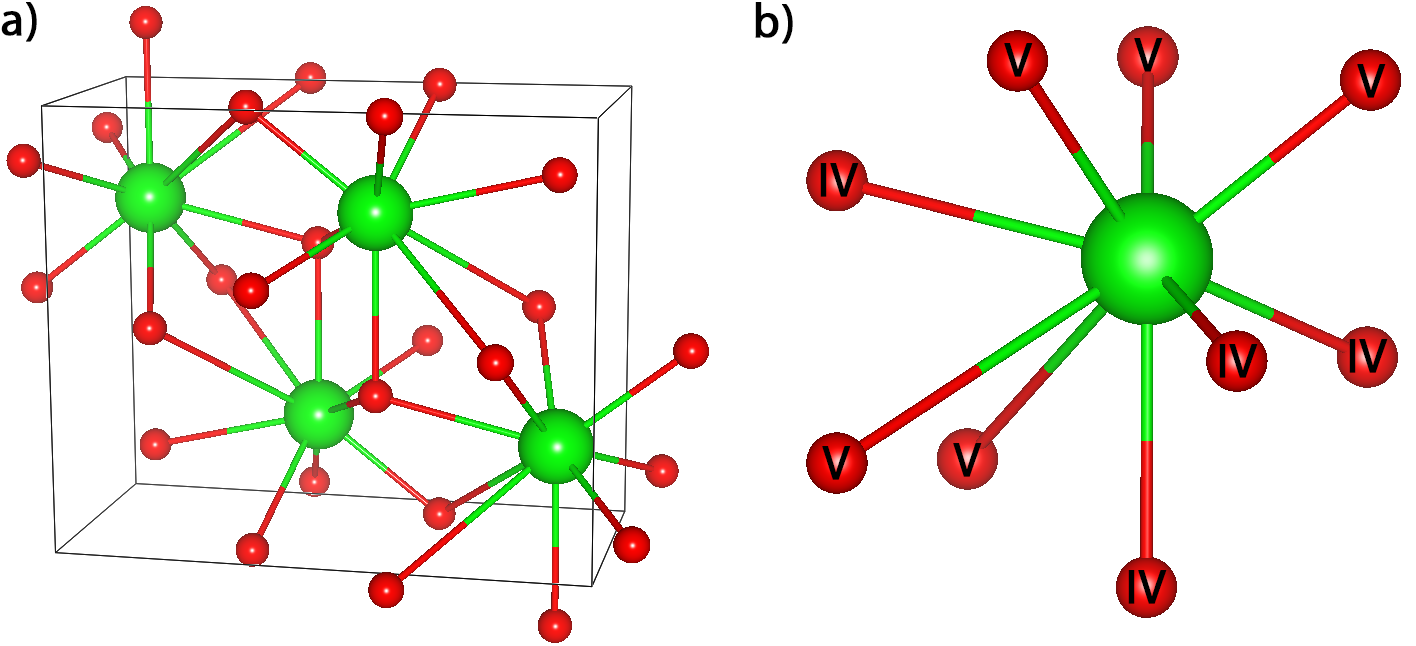
\includegraphics[width=\linewidth]{images/cotunnite_lex.png}
  \caption[Illustration of \textbf{a)} OII cotunnite (P$nma$) unit cell and \textbf{b)} zirconium ion with nearest neighbour oxygens with coordination number indicated. Zirconium and oxygen ions are shaded dark and light respectively.]{Illustration of \textbf{a)} OII cotunnite (P$nma$) unit cell and \textbf{b)} zirconium ion with nearest neighbour oxygens with coordination number indicated. Zirconium and oxygen atoms are coloured green and red respectively. Adapted from \cite{Haines1997}.}
  \label{fig:cotunnite_structure}
\end{figure}

\subsubsection{Hexagonal}

A hexagonal phase of \zirconia\ has been reported in X-ray diffraction studies at high pressure (20 GPa) and above 1000 \textdegree C \cite{ohtaka1994new}. This phase retains its structure during isobaric quenching, but transforms back to the monoclinic phase structure once pressure is released. This phase is only observed under extreme conditions, and so is mentioned here for purposes of completeness.

%\subsubsection*{Volume expansion}

%The phase transitions in \zirconia\ are accompanied by a change in volume, where the monoclinic phase is the least dense and the cubic phase is the most dense (see Figure \ref{figure:zrobonddistance}). This is especially significant in the case of the martensitic t-\zirconia\ to m-\zirconia\ transition, where the volume increases by around 9\% \cite{Gupta1977}. This has substantial implications for the creation and opening of cracks as \zirconia\ is a ceramic material with low toughness. This is especially relevant in a reactor scenario where temperature cycling (shutdown/startup or load-following behaviour) may lead to fatigue if the phase transition threshold is passed.

%Another consequence of this large volume expansion is that a significant hysteresis effect is observed in the monoclinic/tetragonal phase transition, as shown in Figure \ref{fig:phasediagram}. 
%as the resulting coherency strain is likely to result in reduced mobility of fission products that have been embedded in the bulk crystal. 


\section{Dopant stabilisation}

Particular dopant species will stabilise the tetragonal and cubic phases of \zirconia\ to room temperature. The most technologically significant is yttrium, which at concentrations of 15\% (atomic), fully stabilises the cubic phase (which in practical terms means the cubic phase is stable down at least to room temperature). Zirconia stabilised this way is known as yttria-stabilised zirconia (YSZ), also often referred to as partially stabilised zirconia (PSZ). The inclusion of trivalent yttrium promotes the inclusion of charge compensating oxygen vacancy defects (see Equation \ref{equation:YSZ} which uses Kr\"{o}ger-Vink notation, explained in the next section). This works in a similar way with several other cation dopants such as trivalent scandium from Sc$_{2}$O$_{3}$, or divalent magnesium from MgO (Equation \ref{equation:mg_stabilised_zro2}), which also act as cubic stabilisers.

{\setstretch{1.5}
\begin{equation}
\ch{Y_{2}O_{3}} = 2\ch{Y_{Zr}^{'}} + \ch{V_{O}^{**}} + 3\ch{O_{O}^{x}} 
\label{equation:YSZ}
\end{equation}

\begin{equation}
\ch{MgO} = \ch{Mg_{Zr}^{''}} + \ch{V_{O}^{**}} + \ch{O_{O}^{x}} 
\label{equation:mg_stabilised_zro2}
\end{equation}
}

As already discussed above, while MO$_{2}$ oxides (e.g. CeO$_{2}$, UO$_{2}$) often adopt the regular cubic fluorite structure, we only observe cubic stabilisation  of \zirconia\ at elevated temperatures where the effective ionic radii of the zirconium ion increases (possibly due to a stabilising phonon mode contribution \cite{Mirgorodsky1999, Perry1990, Simeone2003}). Yttrium stabilises the cubic phase, not only due to the presence of oxygen vacancies, but because the yttrium ion is of the appropriate size to maintain its surrounding oxygen ions (which may include a vacant oxygen site) in the VIII coordination at low temperatures. This is supported by the ionic radii values in Table \ref{figure:ionicradii} which shows that the Y$^{3+}$ radii are even larger than the Ce$^{4+}$ radii and clearly larger than the corresponding Zr$^{4+}$ radii. 

%This is accomplished by substituting a Zr\textsuperscript{4+} ion with Y\textsuperscript{3+} and the binding of two neighbouring oxygen vacancies, effectively producing a sub-unit of yttria (Y\textsubscript{2}O\textsubscript{3}) in the \zirconia\ lattice. 

\begin{table}[ht]
\onehalfspacing
\centering
\caption[Ionic radii of Zr$^{4+}$, Y$^{3+}$ and Ce$^{4+}$ in various coordination environments.]{Ionic radii of Zr$^{4+}$, Y$^{3+}$ and Ce$^{4+}$ in various coordination environments. Values taken from \cite{Shannon1976}.}
\label{figure:ionicradii}
\begin{tabular}{ccc}
\hline
Ion & Coordination & Ionic Radius (\r{A}) \\ \hline
\multicolumn{1}{c}{\multirow{6}{*}{Zr$^{4+}$}} & \multicolumn{1}{c}{IV} & 0.59 \\
\multicolumn{1}{c}{} & \multicolumn{1}{c}{V} & 0.66 \\
\multicolumn{1}{c}{} & \multicolumn{1}{c}{VI} & 0.72 \\
\multicolumn{1}{c}{} & \multicolumn{1}{c}{VII} & 0.78 \\
\multicolumn{1}{c}{} & \multicolumn{1}{c}{VIII} & 0.84 \\
\multicolumn{1}{c}{} & \multicolumn{1}{c}{IX} & 0.89 \\ \hline
\multicolumn{1}{c}{\multirow{4}{*}{Y$^{3+}$}} & \multicolumn{1}{c}{VI} & 0.90 \\
\multicolumn{1}{c}{} & \multicolumn{1}{c}{VII} & 0.96 \\
\multicolumn{1}{c}{} & \multicolumn{1}{c}{VIII} & 1.019 \\
\multicolumn{1}{c}{} & \multicolumn{1}{c}{IX} & 1.075 \\ \hline
\multicolumn{1}{c}{\multirow{4}{*}{Ce$^{4+}$}} & \multicolumn{1}{c}{VI} & 0.87 \\
\multicolumn{1}{c}{} & \multicolumn{1}{c}{VIII} & 0.97 \\
\multicolumn{1}{c}{} & \multicolumn{1}{c}{X} & 1.07 \\
\multicolumn{1}{c}{} & \multicolumn{1}{c}{XII} & 1.14 \\ \hline
\end{tabular}
\end{table}

\section{Kr\"{o}ger-Vink notation}

Kr\"{o}ger-Vink notation \cite{kroger1956relations} is used throughout this thesis to describe defects. It is widely used in physical chemistry and is a useful shorthand for describing chemical reactions where conservation of mass, charge and lattice sites is required. The notation syntax is of the form \ch{x^{y}_{z}}, where x is the substituted atom or missing atom (i.e. a vacancy V), y is the charge of the defect (relative to the lattice species that originally occupied the site) and z is the site the defect occupies. Positive and negative charges are indicated with dots (\ch{^{*}}) and dashes (\ch{^{'}}) respectively, otherwise a cross (\ch{^{x}}) is used to denote a neutral defect (i.e. the substitutional ion has the same charge as the ion it is replacing). The site may be either a lattice site (such as Zr or O in \zirconia ) or an interstitial site ($i$). Table \ref{table:krogervink} shows examples of several different types of defects and their respective Kr\"{o}ger-Vink notation.

\begin{table}[ht] % Kroger-Vink notation table
\onehalfspacing
\centering
\caption{Examples of Kr\"{o}ger-Vink notation for several defects in \zirconia .}
\label{table:krogervink}
\begin{tabular}{cc}
\hline
Defect & Kr\"{o}ger-Vink Notation \\ \hline
Anion vacancy & \ch{V_{O}^{**}} \\
Cation vacancy & \ch{V_{Zr}^{''''}} \\
Anion interstitial & \ch{O_{i}^{''}} \\
Cation interstitial & \ch{Zr_{i}^{****}} \\
Iodine (I$^{-}$ anion) on oxygen site & \ch{I_{O}^{*}} \\
Iodine (I$^{+}$ cation) on zirconium site & \ch{I_{Zr}^{'''}} \\ \hline
\end{tabular}
\end{table}

 % Complete 
\chapter{Computational Methodology}

\label{ch:compmethodology}

\section{Density functional theory}

Quantum mechanics is the most complete modern theory which describes the behaviour of matter at the energy scale of atoms. It can be used to accurately predict things such as the energy levels of atoms, the interactions of light with matter, and the thermodynamic stability of systems of atoms. Ideally, the mathematical formalisms of quantum mechanics would be used to predict the properties and behaviour of all possible types of molecules and materials. In reality, this is far more difficult to achieve than it sounds, requiring several approximations and abstractions in order to produce a method which, in the end, sacrifices physical accuracy in order to be computationally feasible. The most successful field of study in this domain is that of density functional theory.
% The mathematical formalisms of quantum mechanics must themselves be discretised to be used in computational simulation methods.

\subsection{The Schr\"{o}dinger equation}



\begin{equation}
E\Psi(\textbf{r}) = \hat{H}\Psi(\textbf{r})
\label{equation:schrodinger}
\end{equation}

Where $E$ is the total energy of the system, $\Psi$ is the wave function, and $\hat{H}$ is the energy Hamiltonian operator which includes the kinetic energy contributions ($\hat{T}$) and potential energy contributions ($\hat{V}$), shown in atomic units in equations \ref{equation:kineticcontribution} and \ref{equation:potentialcontribution} respectively:

\begin{gather}
\hat{H} = \hat{T} + \hat{V} \label{equation:hamiltonian}\\
\hat{T} = -\sum_i{\frac{1}{2}}\nabla^2_{r_i} - \sum_i{\frac{1}{2M_i}}\nabla^2_{R_i} \label{equation:kineticcontribution} \\
\hat{V} = \sum_{i,j=i+1}{\frac{1}{2|r_i - r_j|}} + \sum_{i,j=i+1}{\frac{Z_i Z_j}{2|R_i - R_j|}} - \sum_{i,j}{\frac{Z_i}{2|R_i - r_j|}} \label{equation:potentialcontribution}
\end{gather}

\subsection{Kohn-Sham Method}

Density Functional Theory (DFT) was developed by Kohn and Sham in 1964 \cite{Kohn1965} as an ab initio method for solving the wave equation. The Kohn-Sham Hamiltonian (Equation \ref{equation:kohnsham}) is used in the Schr\"odinger equation.

\begin{equation}
\hat{H}(\rho(\textbf{r})) = E_{KE}(\rho(\textbf{r})) + E_{P}(\rho(\textbf{r})) + E_{XC}(\rho(\textbf{r}))
\label{equation:kohnsham}
\end{equation}

Where $E_{KE}$ and $E_{P}$ are the kinetic and potential energy functionals (functions of functions), $\rho$ is the electron density, $E_{XC}$ is the exchange correlation functional, and \textbf{r} is the position vector. The main approximation is to consider that the electrons only interact with nuclei and not other electrons, thus allowing all the terms to be evaluated using the electron density rather than position. An exchange correlation term is then used to include the non-classical electron-electron interactions, namely electron exchange and correlation. Additionally, the exchange correlation term also includes the difference in kinetic energy found due to the use of non-interacting electrons. While Kohn and Sham did provide a proof for the existence of an exchange correlation function, a general form of the functional has not yet been found, although several forms have been considered, each with their own strengths and weaknesses in different systems.

\subsection{Pseudopotentials}

The electron-electron interaction component of the potential energy presents a problem when it comes to scaling experimental models. The number of terms in this interaction grows quadratically with the number of electrons in the system, and quickly becomes computationally intractable for even small systems. However, we know that in chemical reactions, the majority of chemical behaviour is determined by relatively few valence electrons, while the more numerous core electrons have a far smaller effect. Consider the zirconium atom with 40 electrons, of which 4 (4$d^2$5$s^2$) are typically involved in bonding and chemical reactions. A tenfold reduction in the number of electrons which are modelled would provide more than a tenfold reduction in computational requirements. This is what we aim to achieve by using the pseudopotential method. 






\begin{itemize}
\item Only valence electrons contribute to chemical reactions
\item Core electrons influence the size of the ion, but would be too computationally expensive to model them all.
\item Approximate core electron behaviour using an effective 'pseudopotential'.
\end{itemize}

\section{Periodic boundaries}
\subsection{Modelling bulk systems}

A bulk system 

Describing the electron density of a system must be done in the context of a basis set. Any complete basis set (plane-wave, correlation-consistent, split-valence) may be used to represent the behaviour of electron orbitals, but a plane-wave method was chosen due to their greater suitability for periodic systems (plane-waves are intrinsically periodic). 

Figure \ref{Figure:cutoffconvergence} shows the first convergence study where the total energy of simulations with various values of $E_{cutoff}$ were compared to a highly converged value, and then plotted on a log scale to see how precision is improved at larger values.

\begin{figure} % Periodic boundary image
\label{figure:periodicboundary}
\begin{center}
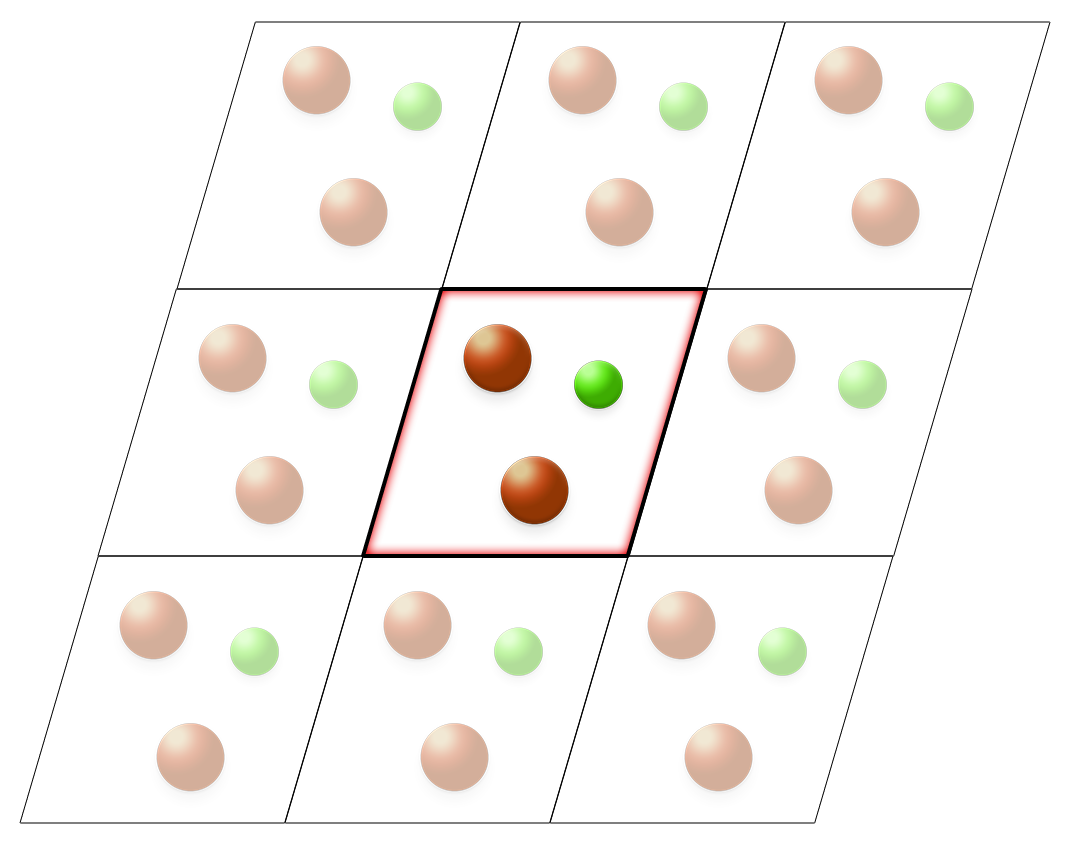
\includegraphics[height=7cm]{images/PeriodicBoundary.png}
\end{center}
\caption{Illustration of periodic boundary around a primitive cell in two dimensions.}
\end{figure}

\subsection{Bloch's theorem}

The repeating nature of crystal structures is well-suited for computer models, as it allows us to define periodicity in three dimensions for a given unit cell. Utilising this periodicity is theoretically justified as follows:

\begin{itemize}

\item Nuclei are arranged in a periodically repeating pattern, thus their potentials acting on electrons are also periodic.

\item If the potential is periodic, it follows that the electron density is also periodic.

\item The electron density is equivalent to the square of the wave function magnitude, thus the magnitude of the wave function is also periodic.

\end{itemize}

Though the magnitude of the wave function is periodic, the phase is not. At this point, we consider Bloch's theorem which states that the possible wave functions are all quasi-periodic, and thus the wave function can be expressed as in Equation \ref{equation:bloch}: 

\begin{equation}
\label{equation:bloch}
\psi_k(\textbf{r}) = e^{i\textbf{k}.\textbf{r}}u_k(\textbf{r})
\end{equation}

Where $\psi_k(\textbf{r})$ is the wave function evaluated at position \textbf{r}, $e^{i\textbf{k}.\textbf{r}}$ is an arbitrary phase factor, and $u_k(\textbf{r})$ is a periodic function with the same periodicity as the wave function. Solutions to this equation exist for any value of \textbf{k} and so the general solution can be expressed as an integral over the first Brillouin zone, the primitive lattice cell in reciprocal space. Instead of evaluating the integral over the range of \textbf{k} (a computationally costly task as it is done for many wave functions), the sum of values at discrete points, known as k-points, is used. This approximation is valid because the wave function varies slowly over \textbf{k}, thus allowing the integral to be approximated with several appropriately space k-points. In general, a finer k-point grid results in increased accuracy at an increased computational cost \cite{Hasnip2010}.

\subsection{Strengths and limitations}

Interaction of defects across the periodic boundary introduces error.

\section{Computational details}
\subsection{Cell dimensions and initialisation (relaxation + tessellation)}

A supercell method is used for the study of various defects. The first step is to create a unit cell of \zirconia\ in each of the three crystal structures. Each unit cell is then relaxed through a geometry optimisation process (see \ref{geometry_optimisation_method}
Supercell details can be found in Table \ref{table:supercells}


\begin{table}[htp] % Supercell details
\doublespacing
\centering
\caption{Composition of the supercells in terms of the number of individual unit cells stacked in each direction.} %Unit cells were stacked in such a way as to produce the most cubic supercell in order to minimise directional defect-defect interactions.}
\label{table:supercells}
\begin{tabular}{cccccccc}
\hline
\multirow{2}{*}{{\bf \begin{tabular}[c]{@{}c@{}}Crystal \\ Structure\end{tabular}}} & \multicolumn{3}{c}{{\bf No. unit cells}} & \multicolumn{3}{c}{{\bf Supercell size (\AA)}} & \multirow{2}{*}{{\bf \begin{tabular}[c]{@{}c@{}}No.\\ atoms\end{tabular}}} \\ \cline{2-7}
 & \hspace{0.25 cm} a \hspace{0.2 cm} & b & c & a \hspace{0.0 cm} & b & c \hspace{0.35 cm} &  \\ \hline
\begin{tabular}[c]{@{}c@{}}Monoclinic\\ ($P2_1/c$)\end{tabular} & 2 & 2 & 2 & 10.37 & 10.47 & 10.75 & 96 \\ \hline
\begin{tabular}[c]{@{}c@{}}Tetragonal\\ ($P4_2/nmc$)\end{tabular} & 3 & 3 & 2 & 10.85 & 10.85 & 10.56 & 108 \\ \hline
\begin{tabular}[c]{@{}c@{}}Cubic\\ ($Fm\overline{3}m$)\end{tabular} & 2 & 2 & 2 & 10.22 & 10.22 & 10.22 & 96 \\ \hline
\end{tabular}
\end{table}

\subsection{Geometry optimisation method and parameters} \label{geometry_optimisation_method}

\subsubsection*{Born-Oppenheimer approximation}

The Born-Oppenheimer approximation is a two-step process for evaluating atomic forces which greatly reduces the computational costs of any atomistic simulation. It exploits the large difference in mass between nuclei and electrons in order to separate their interactions. This allows us to decompose the total wave function into a product of an electronic wave function and a nuclear wave function via a separation of variables approach. The first step involves ignoring the kinetic energy contribution of nuclei by assuming they are stationary, thus we can remove the nuclear kinetic energy term in Equation \ref{equation:kineticcontribution}. The stationary nuclei assumption also simplifies the nuclear-nuclear Coulombic repulsion term in Equation \ref{equation:potentialcontribution} because $|R_i - R_j|$ becomes a constant throughout the calculation. An electronic Schr\"{o}dinger equation is then solved where electronic positions are variables and nuclear positions are fixed parameters. This solution contains information of the shape of the electronic orbitals. The next step is to take the electronic distribution and calculate the resultant forces on the nuclei. The nuclear positions are then modified to try to minimise these forces, followed by feeding these nuclear positions back into the electronic Schr\"{o}dinger equation to obtain the new electronic distribution. This process is repeated until the required convergence criterion (energy change per iteration, forces on nuclei) are satisfied.

\subsection{Convergence criteria}

\begin{itemize}
\item force per ion
\item energy per ion
\item maximum displacement
\end{itemize}


\subsection{Charged cell correction}

\begin{itemize}
\item Makov-Payne correction
\item Brouwer diagram script uses screened Madelung constant for the calculation
\end{itemize}

\subsection{Stiffness tensor generation}

\begin{itemize}
\item Calculate DFT energies of unit cell with small strains in various directions
\item Use relative change in stress to calculate elastic constants in the form of a 6x6 tensor
\end{itemize}

\subsection{Strain method for defect volumes}

The volumes of the defective supercells were kept constant because constant pressure calculations have been shown to break the symmetry of the supercell \cite{samanta2010thermodynamic}, leading to unreliable energy values. The approach to calculating defect volumes relies on calculating the elastic constants of the non-defective supercell, followed by extracting the resultant stress tensor from a defect simulation. The strain tensor of the defective cell can then be calculated using Hooke's law, giving the relaxation volume. 

\subsection{Isobaric method for defect volumes}

It is also possible to calculate defect volumes using an isobaric method. This method is more simple than the strain method as there is no need to determine the elastic constants, reducing the number of geometry optimisation jobs from X to 2. 

CASTEP provides the volume of the cell, defined as the (volume enclosed by the calculated lattice parameters? Or the volume within the boundary of the outermost atoms)

\subsection{Effect of space charge}

Diffusion rate of oxygen vacancies compared to electrons lead to a resultant charge in the lattice.

\begin{figure}[htp] % Tet conc sweep with space charge 1e-1
\begin{center}
\begin{tikzpicture}
	\begin{axis}
		[width=8.22cm, xlabel={\ch{log_{10}}($p_{O_{2}}$) (atm)}, ylabel={\ch{log_{10}}([D]) (per f.u.)}, ymin=-10, ymax=0, xmin=-35, xmax=0, legend style={{draw=}, at={(0.40,0.97)}, anchor=north west, legend columns=3, nodes={scale=0.75, transform shape}}]
        \addplot[no marks, draw=blue!70!black] table [x=pO2, y=electrons,]{dat/1e5iconctet1500_sc_e-1.dat}; \addlegendentry{\ch{e^{'}}}; %\node at (-26.0,-1.9) {\ch{e^{'}}};
        \addplot[no marks, draw=red!85!black] table [x=pO2, y=holes,]{dat/1e5iconctet1500_sc_e-1.dat}; \addlegendentry{\ch{h^{\textperiodcentered}}}; %\node at (-7,-3.6) {\ch{h^{\textperiodcentered}}};
        \addplot[no marks, draw=black!70!green] table [x=pO2, y=VO{2},]{dat/1e5iconctet1500_sc_e-1.dat}; \addlegendentry{\ch{V_{O}^{\textperiodcentered\textperiodcentered}}}; %\node at (-26.7,-3.3) {\ch{V_{O}^{\textperiodcentered\textperiodcentered}}};
%         \addplot[no marks, draw=black!55!green] table [x=pO2, y=VO{1},]{dat/1e5iconctet1500_sc_e-1.dat}; \addlegendentry{\ch{V_{O}^{\textperiodcentered}}};
%         \addplot[no marks, draw=black!30!green] table [x=pO2, y=VO{0},]{dat/1e5iconctet1500_sc_e-1.dat}; \addlegendentry{\ch{V_{O}^{x}}};
        \addplot[no marks, draw=yellow!85!blue] table [x=pO2, y=VM{-4},]{dat/1e5iconctet1500_sc_e-1.dat}; \addlegendentry{\ch{V_{Zr}^{''''}}};
%         \addplot[no marks, draw=yellow!75!blue] table [x=pO2, y=VM{-3},]{dat/1e5iconctet1500_sc_e-1.dat}; \addlegendentry{\ch{V_{Zr}^{'''}}};
%         \addplot[no marks, draw=yellow!65!blue] table [x=pO2, y=VM{-2},]{dat/1e5iconctet1500_sc_e-1.dat}; \addlegendentry{\ch{V_{Zr}^{''}}};
%         \addplot[no marks, draw=yellow!55!blue] table [x=pO2, y=VM{-1},]{dat/1e5iconctet1500_sc_e-1.dat}; \addlegendentry{\ch{V_{Zr}^{'}}};
%         \addplot[no marks, draw=yellow!45!blue] table [x=pO2, y=VM{0},]{dat/1e5iconctet1500_sc_e-1.dat}; \addlegendentry{\ch{V_{Zr}^{x}}};
%         \addplot[no marks, draw=red!60!yellow] table [x=pO2, y=Oi{-2},]{dat/1e5iconctet1500_sc_e-1.dat}; \addlegendentry{\ch{O_{i}^{''}}};
%         \addplot[no marks, draw=red!50!yellow] table [x=pO2, y=Oi{-1},]{dat/1e5iconctet1500_sc_e-1.dat}; \addlegendentry{\ch{O_{i}^{'}}};
%         \addplot[no marks, draw=red!40!yellow] table [x=pO2, y=Oi{0},]{dat/1e5iconctet1500_sc_e-1.dat}; \addlegendentry{\ch{O_{i}^{x}}};
%         \addplot[no marks, draw=green!80!pink] table [x=pO2, y=Mi{4},]{dat/1e5iconctet1500_sc_e-1.dat}; \addlegendentry{\ch{Zr_{i}^{\textperiodcentered\textperiodcentered\textperiodcentered\textperiodcentered}}};
%         \addplot[no marks, draw=green!70!pink] table [x=pO2, y=Mi{3},]{dat/1e5iconctet1500_sc_e-1.dat}; \addlegendentry{\ch{Zr_{i}^{\textperiodcentered\textperiodcentered\textperiodcentered}}};
%         \addplot[no marks, draw=green!60!pink] table [x=pO2, y=Mi{2},]{dat/1e5iconctet1500_sc_e-1.dat}; \addlegendentry{\ch{Zr_{i}^{\textbf{\textperiodcentered\textperiodcentered}}}};
%         \addplot[no marks, draw=green!50!pink] table [x=pO2, y=Mi{1},]{dat/1e5iconctet1500_sc_e-1.dat}; \addlegendentry{\ch{Zr_{i}^{\textperiodcentered}}};
%         \addplot[no marks, draw=green!40!pink] table [x=pO2, y=Mi{0},]{dat/1e5iconctet1500_sc_e-1.dat}; \addlegendentry{\ch{Zr_{i}^{x}}};
%         \addplot[no marks, dashed, draw=red!70!black] table [x=pO2, y=Ii{0},]{dat/1e5iconctet1500_sc_e-1.dat}; \addlegendentry{\ch{I_{i}^{x}}};
%         \addplot[no marks, dashed, draw=red!50!black] table [x=pO2, y=Ii{-1},]{dat/1e5iconctet1500_sc_e-1.dat}; \addlegendentry{\ch{I_{i}^{'}}};
        \addplot[no marks, dashed, draw=purple] table [x=pO2, y=Ii{1},]{dat/1e5iconctet1500_sc_e-1.dat}; \addlegendentry{\ch{I_{i}^{\textperiodcentered}}};
        \addplot[no marks, dashed, draw=blue!50!white] table [x=pO2, y=IsubO{1},]{dat/1e5iconctet1500_sc_e-1.dat}; \addlegendentry{\ch{I_{O}^{\textperiodcentered}}};
        \addplot[no marks, dashed, draw=green!60!black] table [x=pO2, y=IsubO{2},]{dat/1e5iconctet1500_sc_e-1.dat}; \addlegendentry{\ch{I_{O}^{\textperiodcentered\textperiodcentered}}};
        \addplot[no marks, dashed, draw=black] table [x=pO2, y=IsubO{3},]{dat/1e5iconctet1500_sc_e-1.dat}; \addlegendentry{\ch{I_{O}^{\textperiodcentered\textperiodcentered\textperiodcentered}}};
        \addplot[no marks, dashed, draw=orange!80!black] table [x=pO2, y=IsubZr{-3},]{dat/1e5iconctet1500_sc_e-1.dat}; \addlegendentry{\ch{I_{Zr}^{'''}}};
%         \addplot[no marks, dashed, draw=pink] table [x=pO2, y=IsubZr{-4},]{dat/1e5iconctet1500_sc_e-1.dat}; \addlegendentry{\ch{I_{Zr}^{''''}}};
%         \addplot[no marks, dashed, draw=purple] table [x=pO2, y=IsubZr{-5},]{dat/1e5iconctet1500_sc_e-1.dat}; \addlegendentry{\ch{I_{Zr}^{'''''}}};
%         \addplot[no marks] table [x=pO2, y=Stoich,]{dat/1e5iconctet1500_sc_e-1.dat}; \addlegendentry{Stoich};
%\node at (-33.7,-0.5) {\textbf{a)}};
			\end{axis}            
\end{tikzpicture}
\begin{tikzpicture} % 1e-1
	\begin{axis}
		[width=8.22cm, xlabel={\ch{log_{10}}($p_{O_{2}}$) (atm)}, yticklabels={}, ymin=-10, ymax=0, xmin=-35, xmax=0]
        \addplot[no marks, draw=blue!70!black] table [x=pO2, y=electrons,]{dat/1e3iconctet1500_sc_e-1.dat}; %\node at (-27,-1.7) {\ch{e^{'}}};
        \addplot[no marks, draw=red!85!black] table [x=pO2, y=holes,]{dat/1e3iconctet1500_sc_e-1.dat}; %\node at (-2.5,-2.1) {\ch{h^{\textperiodcentered}}};
        \addplot[no marks, draw=black!70!green] table [x=pO2, y=VO{2},]{dat/1e3iconctet1500_sc_e-1.dat}; 
%         \addplot[no marks, draw=black!55!green] table [x=pO2, y=VO{1},]{dat/1e3iconctet1500_sc_e-1.dat}; 
%         \addplot[no marks, draw=black!30!green] table [x=pO2, y=VO{0},]{dat/1e3iconctet1500_sc_e-1.dat}; 
        \addplot[no marks, draw=yellow!85!blue] table [x=pO2, y=VM{-4},]{dat/1e3iconctet1500_sc_e-1.dat}; 
%         \addplot[no marks, draw=yellow!75!blue] table [x=pO2, y=VM{-3},]{dat/1e3iconctet1500_sc_e-1.dat}; 
%         \addplot[no marks, draw=yellow!65!blue] table [x=pO2, y=VM{-2},]{dat/1e3iconctet1500_sc_e-1.dat}; 
%         \addplot[no marks, draw=yellow!55!blue] table [x=pO2, y=VM{-1},]{dat/1e3iconctet1500_sc_e-1.dat}; 
%         \addplot[no marks, draw=yellow!45!blue] table [x=pO2, y=VM{0},]{dat/1e3iconctet1500_sc_e-1.dat}; 
%         \addplot[no marks, draw=red!60!yellow] table [x=pO2, y=Oi{-2},]{dat/1e3iconctet1500_sc_e-1.dat}; 
%         \addplot[no marks, draw=red!50!yellow] table [x=pO2, y=Oi{-1},]{dat/1e3iconctet1500_sc_e-1.dat}; 
%         \addplot[no marks, draw=red!40!yellow] table [x=pO2, y=Oi{0},]{dat/1e3iconctet1500_sc_e-1.dat}; 
%         \addplot[no marks, draw=green!80!pink] table [x=pO2, y=Mi{4},]{dat/1e3iconctet1500_sc_e-1.dat}; 
%         \addplot[no marks, draw=green!70!pink] table [x=pO2, y=Mi{3},]{dat/1e3iconctet1500_sc_e-1.dat}; 
%         \addplot[no marks, draw=green!60!pink] table [x=pO2, y=Mi{2},]{dat/1e3iconctet1500_sc_e-1.dat}; 
%         \addplot[no marks, draw=green!50!pink] table [x=pO2, y=Mi{1},]{dat/1e3iconctet1500_sc_e-1.dat}; 
%         \addplot[no marks, draw=green!40!pink] table [x=pO2, y=Mi{0},]{dat/1e3iconctet1500_sc_e-1.dat}; 
%         \addplot[no marks, dashed, draw=red!70!black] table [x=pO2, y=Ii{0},]{dat/1e3iconctet1500_sc_e-1.dat}; 
%         \addplot[no marks, dashed, draw=red!50!black] table [x=pO2, y=Ii{-1},]{dat/1e3iconctet1500_sc_e-1.dat}; 
        \addplot[no marks, dashed, draw=purple] table [x=pO2, y=Ii{1},]{dat/1e3iconctet1500_sc_e-1.dat}; 
        \addplot[no marks, dashed, draw=blue!50!white] table [x=pO2, y=IsubO{1},]{dat/1e3iconctet1500_sc_e-1.dat}; %\node at (-11,-2.6) {\ch{I_{O}^{\textperiodcentered}}};
        \addplot[no marks, dashed, draw=green!60!black] table [x=pO2, y=IsubO{2},]{dat/1e3iconctet1500_sc_e-1.dat}; 
        \addplot[no marks, dashed, draw=black] table [x=pO2, y=IsubO{3},]{dat/1e3iconctet1500_sc_e-1.dat}; 
        \addplot[no marks, dashed, draw=orange!80!black] table [x=pO2, y=IsubZr{-3},]{dat/1e3iconctet1500_sc_e-1.dat}; 
%         \addplot[no marks, dashed, draw=pink] table [x=pO2, y=IsubZr{-4},]{dat/1e3iconctet1500_sc_e-1.dat}; 
%         \addplot[no marks, dashed, draw=purple] table [x=pO2, y=IsubZr{-5},]{dat/1e3iconctet1500_sc_e-1.dat}; 
%         \addplot[no marks] table [x=pO2, y=Stoich,]{dat/1e3iconctet1500_sc_e-1.dat}; 
%\node at (-33.7,-0.5) {\textbf{b)}};
			\end{axis}            
\end{tikzpicture}
		\caption{Tetragonal phase Brouwer diagrams of point defects at iodine concentrations of a) $10^{-5}$ and b) $10^{-3}$, at a temperature of 1500 K. Space charge = +1e-1}
		%\label{figure:tikzbrouwerconctet}
	\end{center}
\end{figure}

\section{Convergence testing}

\subsection{Plane-wave cut-off energy}

\begin{figure}
	\begin{center}
		\begin{tikzpicture}
			\begin{axis}
				[width=12cm, xlabel={E\textsubscript{cutoff} (eV)}, ylabel={log(error) / formula unit}, ymin=-3.5, legend style={{draw=}, at={(0.95,0.95)}, anchor=north east,}]
				\addplot[no marks] table [x=cutoffenergy, y=logerrormono,]{dat/convergence.dat}; \addlegendentry{Monoclinic};
			    \addplot[no marks, dashed] table [x=cutoffenergy, y=logerrortet,]{dat/convergence.dat}; \addlegendentry{Tetragonal};
			    \addplot[no marks, densely dotted] table [x=cutoffenergy, y=logerrorcubic,]{dat/convergence.dat}; \addlegendentry{Cubic};
                \draw[red,-stealth]
				(600,-1.96)
				-- % = line-to
				++ % = calculate a vector sum
				(axis direction cs:0,-1.46);
                \addplot [only marks,mark=*]
coordinates { (600,-1.95) };
			\end{axis}
		\end{tikzpicture}
		\caption{Plot of the log error of DFT energy against plane-wave cut-off energy for a perfect cell of each crystal structure. The error is calculated with respect to a highly converged value.}
		\label{Figure:cutoffconvergence}
	\end{center}
\end{figure}

\subsection{k-point convergence}

Too fine a grid in reciprocal space (i.e. a large number of k-points) leads to very computationally expensive simulations, whereas too coarse a grid may have a large truncation error when energies are calculated. To find the optimum spacing of k-points, a convergence study was performed across a range of k-point spacings, with the output energies compared to a highly converged simulation to obtain a value for the error. 

Figure \ref{Figure:kpoint_convergence} shows the energy error in each phase of \zirconia\ as a function of the k-point spacing (given in reciprocal space as \r{A}$^{-1}$). The highly converged energy value was calculated with a k-point spacing of 0.01 \r{A}$^{-1}$ for error calculations. The plot shows a stepwise change in the error value as grid spacing is reduced because there must be an integer number of k-points, but larger spacings do not provide sufficient resolution to effectively fit an integer number of k-points into the reciprocal grid, snapping to the nearest appropriate grid instead. An optimum k-point spacing was chosen at 0.09 \r{A}$^{-1}$, which was the largest spacing that kept the error below 0.01 eV for all phases, highlighted in the plot by the red arrow.

\begin{figure}
\begin{center}
\begin{tikzpicture}
	\begin{axis}
		[width=12cm, xlabel={k-point spacing (\r{A}\textsuperscript{-1})}, ylabel={log[error]}, ymin=-7, ymax=1, xmin=0, xmax=0.22, legend style={{draw=}, at={(0.05,0.95)}, anchor=north west, legend columns=1}, xticklabel
style={/pgf/number format/.cd,fixed,precision=5}]
		\addplot[no marks] table [x=kpoint_spacing, y=monoclinic,]{dat/kpoint_convergence.dat}; \addlegendentry{Monoclinic};
        \addplot[no marks, dashed] table [x=kpoint_spacing, y=tetragonal, ]{dat/kpoint_convergence.dat}; \addlegendentry{Tetragonal};
        \addplot[no marks, densely dotted] table [x=kpoint_spacing, y=cubic,]{dat/kpoint_convergence.dat}; \addlegendentry{Cubic};
        \draw[red,-stealth]
				(0.09,-2.35)
				-- % = line-to
				++ % = calculate a vector sum
				(axis direction cs:0,-4.6);
                \addplot [only marks,mark=*]
coordinates { (0.09,-2.35) };
			\end{axis}
		\end{tikzpicture}
		\caption{Error in the total energy of the system as a function of k-point spacing. The error is calculated relative to a highly converged energy value at a k-point spacing of 0.01\r{A}\textsuperscript{-1}. Red arrow indicates the k-point spacing which reduces error below 2 d.p for all structures.}
		\label{Figure:kpoint_convergence}
	\end{center}
\end{figure}

\subsection{Exchange-correlation functionals}

\subsection{On-the-fly pseudopotentials}

Ultra soft pseudopotentials are generated in CASTEP automatically (known as on-the-fly or OTF pseudopotentials) when none are specified for a particular element. Energies must be calculated and compared with the same set of pseudopotentials in order to keep simulations self-consistent. A quick single point calculation was performed on a unit cell of \zirconia\ and the resulting OTF pseudopotentials were saved and used for all subsequent calculations. It is important to determine the variance in energy values of different pseudopotentials generated in this way in order to avoid systematic error.

\subsection{Unit cells}

\begin{table}[htp] % Unit cell parameters
\onehalfspacing
\centering
\caption{Calculated unit cell parameters for the different crystal structures of \zirconia . Experimental data for pure monoclinic and stabilised tetragonal and cubic phases at 295 K are shown in parentheses \cite{Howard1988}. Energy difference between structures is shown with respect to the cubic phase.}
\label{lattice_params}
\begin{tabular}{ccccccc}
\hline Phase    & a (\AA) & b (\AA) & c (\AA) & $\beta$ ($\degree$) & Volume (\AA\textsuperscript{3}/f.u.) & $\Delta$E (eV/f.u.) \\ \hline
m-\zirconia   &    5.18 (5.15)          &    5.24 (5.21)         &    5.37 (5.32)         & 99.63 (99.23)             &       35.96 (35.22)                 &    -0.215              \\
t-\zirconia &    3.62 (3.61)         &              &    5.28  (5.18)        & 90             &   34.54 (33.67)                      &     -0.105             \\
c-\zirconia        &   5.11 (5.09)           &              &              & 90             &     33.38 (32.89)                   &      N/A     \\ \hline      
\end{tabular}
\end{table}


\subsection{Chemical potential of iodine}

To determine the chemical potential of iodine, an energy minimisation of the iodine dimer was performed. Unlike oxygen, iodine dimers do not exhibit a resultant magnetic moment, thus avoiding a source of error in energy calculations with the PBE exchange-correlation functional. Much like with the \zirconia\ unit cells, the lattice parameter after relaxation (bond length in this case) is checked to determine the deviation from an experimental value.

Figure \ref{figure:iodine_dimer} illustrates the energy minimisation of two iodine atoms in a large cell, initially separated by 3.0 \r{A}. The simulation finds an energy minima when the iodine atoms are bonded, at a separation of 2.69 \r{A}. This is in good agreement with the experimental value of 2.6745 \r{A}.

\begin{figure}[htp] % Iodine dimer geometry optimisation
\centering
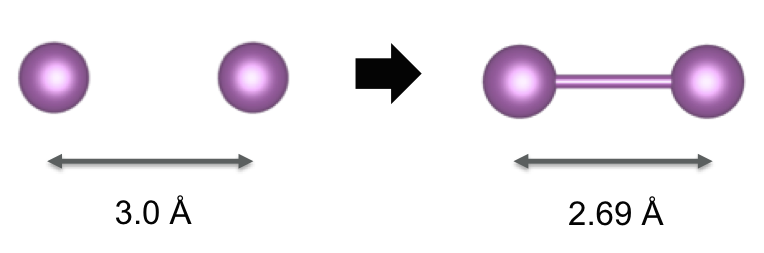
\includegraphics[height=3.5cm]{images/iodine_geom.png}
\caption{Energy minimisation of two iodine atoms from an initial separation of 3.0 \r{A}.}
\label{figure:iodine_dimer}
\end{figure}

\subsection{+U study}

In some DFT studies, an additional potential energy term is sometimes included to better capture the Coulomb interaction of localised electrons. An LDA or GGA functional alone will typically not describe this interaction correctly, especially for localised $d$ and $f$ electrons. Of particular concern was the calculated value of the band gap from DFT simulations, as this value may deviate by up to 30\% from experimental values. Remedying this shortcoming with an appropriate +U parameter could therefore be valuable in obtaining accurate energies. A +U study of the zirconium atom, with an electronic configuration of [Kr]$4d^{2}5s^{2}$, was performed to determine the response to and therefore the viability of an additional potential term for the $d$ electrons.

\begin{figure}[htp] % +U band gaps
\begin{center}
\begin{tikzpicture}
	\begin{axis}
		[width=11cm, xlabel={+U on Zr \emph{d} orbitals (eV)}, ylabel={Lattice parameter (\r{A})}, ymin=3.2, ymax=5, xmin=0, xmax=12, legend style={{draw=}, at={(0.35,0.95)}, anchor=north east, legend columns=1}]
		\addplot[no marks] table [x=plusU, y=bandgap,]{dat/plus_u_mono.dat}; \addlegendentry{Monoclinic};
        \addplot[no marks, dashed] table [x=plusU, y=bandgap, ]{dat/plus_u_tet.dat}; \addlegendentry{Tetragonal};
        \addplot[no marks, densely dotted, black] table [x=plusU, y=bandgap,]{dat/plus_u_cubic.dat}; \addlegendentry{Cubic};
			\end{axis}
		\end{tikzpicture}
		\caption{Calculated band gaps for different +U values in monoclinic, tetragonal and cubic \zirconia .}
		\label{Figure:plusubandgap}
	\end{center}
\end{figure}

\begin{figure}[htp] % +U mono
\begin{center}
\begin{tikzpicture}
	\begin{axis}
		[width=11cm, xlabel={+U on Zr \emph{d} orbitals (eV)}, ylabel={Lattice parameter (\r{A})}, ymin=4.9, ymax=6.3, xmin=0, xmax=12, legend style={{draw=}, at={(0.18,0.95)}, anchor=north east, legend columns=1}]
		\addplot[no marks] table [x=plusU, y=a,]{dat/plus_u_mono.dat}; \addlegendentry{$a$};
        \addplot[no marks, dashed] table [x=plusU, y=b, ]{dat/plus_u_mono.dat}; \addlegendentry{$b$};
        \addplot[no marks, densely dotted, black] table [x=plusU, y=c,]{dat/plus_u_mono.dat}; \addlegendentry{$c$};
			\end{axis}
		\end{tikzpicture}
		\caption{Individual lattice parameters as a function of +U term in monoclinic \zirconia .}
		\label{Figure:plusumono}
	\end{center}
\end{figure}

\begin{figure}[htp] % +U tet
\begin{center}
\begin{tikzpicture}
	\begin{axis}
		[width=11cm, xlabel={+U on Zr \emph{d} orbitals (eV)}, ylabel={$a$ parameter (\r{A})}, ymin=3.6, ymax=3.8, xmin=0, xmax=12, legend style={{draw=}, at={(0.18,0.95)}, anchor=north east, legend columns=1}, tick pos=left]
		\addplot[no marks] table [x=plusU, y=a,]{dat/plus_u_tet.dat}; \addlegendentry{$a$};
        %\addplot[no marks, dashed] table [x=plusU, y=b, ]{dat/plus_u_tet.dat}; \addlegendentry{b};
        \addplot[no marks, dashed, black] table [x=plusU, y=c,]{dat/plus_u_tet.dat}; \addlegendentry{$c$};
			\end{axis}
            \begin{axis}[width=11cm,
     xmin = 0, xmax = 12,
     ymin = 5.16, ymax = 5.32,
     hide x axis,
     hide y axis, tick pos=right]
     \addplot[no marks, dashed, black] table [x=plusU, y=c,]{dat/plus_u_tet.dat};
   			\end{axis}
            \pgfplotsset{every axis y label/.append style={rotate=180}}
   \begin{axis}[width=11cm,
         xmin=0, xmax=12,
         ymin=5.16, ymax=5.32,
         hide x axis,
         axis y line*=right,
         ylabel={$c$ parameter (\r{A})}
     ]
   \end{axis}
		\end{tikzpicture}
		\caption{Individual lattice parameters as a function of +U term in tetragonal \zirconia .}
		\label{Figure:plusutet}
	\end{center}
\end{figure}

\begin{figure}[htp] % +U cubic
\begin{center}
\begin{tikzpicture}
	\begin{axis}
		[width=11cm, xlabel={+U on Zr \emph{d} orbitals (eV)}, ylabel={Lattice parameter (\r{A})}, ymin=5.1, ymax=5.35, xmin=0, xmax=12, legend style={{draw=}, at={(0.18,0.95)}, anchor=north east, legend columns=1}]
		\addplot[no marks] table [x=plusU, y=a,]{dat/plus_u_cubic.dat}; \addlegendentry{$a$};
        %\addplot[no marks, dashed] table [x=plusU, y=b, ]{dat/plus_u_cubic.dat}; \addlegendentry{b};
        %\addplot[no marks, densely dotted, black] table [x=plusU, y=c,]{dat/plus_u_cubic.dat}; \addlegendentry{c};
			\end{axis}
		\end{tikzpicture}
		\caption{Individual lattice parameters as a function of +U term in cubic \zirconia .}
		\label{Figure:plusucubic}
	\end{center}
\end{figure} % Good
%\chapter{Defects}

\label{ch:defects}

\section{Frenkel and Schottky defects}

\subsection{Incorporation and defect formation energies}

\subsubsection*{Isolated Frenkel defects}

Zr and O Frenkel defect formation energies were determined via point defect DFT calculations for the three structures. The formation energies of the isolated Frenkel defect pairs were defined as:
% Interstitial iodine defects were simulated in the neutral charge state at different interstitial sites in each phase. The incorporation energy of these defects, assuming a perfect lattice, was calculated using Equation \ref{equation_incorporation}:

\begin{equation}
\label{equation_frenkel}
E_{Frenkel} = E_{DFT}(V^{q}_{X}) + E_{DFT}(X^{-q}_{i}) - 2E_{DFT}(ZrO_2)% - \frac{E_{I_2}}{2}
\end{equation}

where $X$ is either Zr or O, $E_{DFT}(V^{q}_{X})$ is the energy of a supercell of \zirconia\ containing a single vacancy of charge $q$, $E_{DFT}(X^{-q}_{i})$ is the energy of a supercell of \zirconia\ containing a single interstitial with opposing charge $-q$, and $E_{DFT}(ZrO_2)$ is the energy of the non-defective supercell. Charges ranged from the fully charged case (+2 for oxygen vacancies, -4 for zirconium vacancies) to neutral. The interstitial sites, shown in Table \ref{table:interstitials}, were chosen based on standard vacant Wyckoff positions in each crystal structure \cite{theo1996international}.  In the case of oxygen vacancies in monoclinic \zirconia , a defect energy was obtained for both the (III) and (IV) co-ordinated oxygen sites, with the lowest energy value being used in the calculation of the Frenkel defect energy.

\begin{table}[htp] % Wyckoff positions of interstitials
\onehalfspacing
\centering
\caption{Wyckoff positions of interstitial sites used for each crystal structure.}
\label{table:interstitials}
\begin{tabular}{lcc}
\hline
\hspace{0.7 cm} {\bf Crystal Structure} \hspace{0.7 cm}                              & \hspace{0.7 cm} {\bf Interstitial Sites} \hspace{0.7 cm}                                               \\ \hline
\multicolumn{1}{c}{Monoclinic}              & $2a$, $2b$, $2c$, $2d$ \\
\multicolumn{1}{c}{Tetragonal}            & $2b$, $8e$                                   \\
\multicolumn{1}{c}{Cubic}       & $24d$, $4b$                                          \\ \hline
\end{tabular}
\end{table}

\subsubsection*{Isolated Schottky Defects}

Three Schottky energies were calculated for each structure, corresponding to fully charged, partially charged, and uncharged point defect energies. The Schottky formation energy was defined as:

\begin{equation}
\label{equation_schottky}
E_{Schottky} = E_{DFT}(V^{-2q}_{Zr}) + 2E_{DFT}(V^{q}_{O}) -\frac{3(n-1)}{n}E_{DFT}(ZrO_2)% - \frac{E_{I_2}}{2}
\end{equation}

where $n$ denotes the number of atoms in the supercell, $V^{q}_{O}$ denotes an oxygen vacancy with charge $q$, and $q$ varies from 2 to 0. This form maintains both the mass and charge balance of the Schottky defect description for \zirconia :

\begin{equation}
\label{generic_schottky}
Zr^{x}_{Zr} + 2O^{x}_{O} = V^{-2q}_{Zr} + 2V^{q}_{O} + ZrO_{2}
\end{equation}

This implies a rearrangement rather than complete removal of ions from the system. As with the Frenkel defects, the lowest energy vacancy energies were used to calculate Schottky formation energies. While there are multiple configurations of Schottky defects, such nuance cannot be accurately represented through a sum of individual vacancy defect energies. The values we present for Schottky defect formation energies should therefore be considered the lower bound for defect formation. 

\subsubsection*{Bound Frenkel Defects}

Bound Zr and O Frenkel defect formation energies in the three structures were calculated from DFT energies of supercells where a single ion was moved from its lattice site to an interstitial site. The formation energies of the bound Frenkel defect pairs were defined as:
% Interstitial iodine defects were simulated in the neutral charge state at different interstitial sites in each phase. The incorporation energy of these defects, assuming a perfect lattice, was calculated using Equation \ref{equation_incorporation}:

\begin{equation}
\label{equation_frenkel_bound}
E_{BoundFrenkel} = E_{DFT}(BoundFrenkel) - E_{DFT}(ZrO_2)% - \frac{E_{I_2}}{2}
\end{equation}

where $E_{DFT}(BoundFrenkel)$ is the energy of a supercell of \zirconia\ containing both a vacancy and interstitial defect of the same ion. The two defects were placed as far apart in the supercell as possible (7-8 \r{A}) to avoid recombination. The interstitial defect is assumed to fully compensate the charge of the vacancy defect, resulting in no overall charge on the supercell. The number and type of ions in the defective and non-defective supercell are the same, requiring no further steps to calculate the formation energy.
%Charges ranged from the fully charged case (+2 for oxygen, -4 for zirconium) to neutral. The interstitial sites, shown in Table \ref{table:interstitials}, were chosen based on standard vacant Wyckoff positions in each crystal structure \cite{theo1996international}.  In the case of oxygen vacancies in monoclinic \zirconia , a defect energy was obtained for both the (III) and (IV) co-ordinated oxygen sites. The lowest energies were used in the calculation of the Frenkel defect energy.

\subsubsection*{Bound Schottky Defects}


\begin{figure}[htp] % Tet Zr centre
\centering
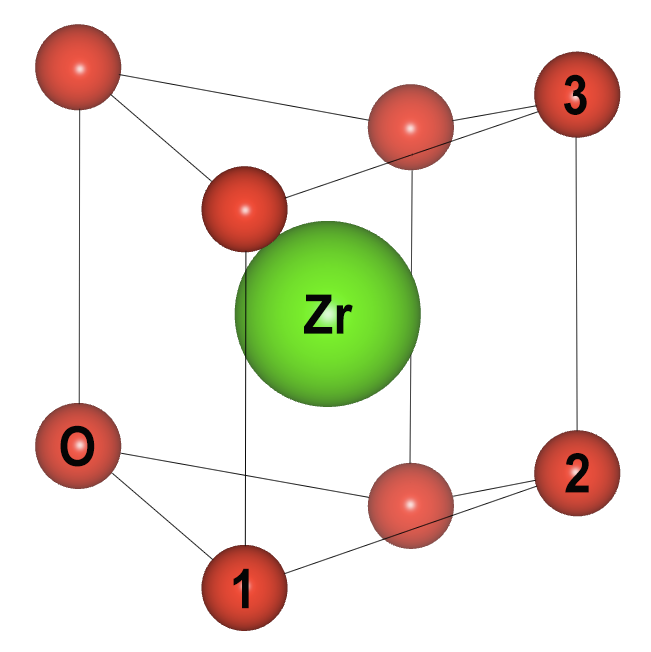
\includegraphics[width=8cm]{images/zr_centre_tet.png}
\caption{Zirconium centre showing nearest oxygen atoms in tetragonal \zirconia. Schottky trios indicated by oxygen enumeration. Zirconium atoms are shown in green and oxygen atoms in red.}
\label{figure:tetschottky}
\end{figure}

\begin{figure}[htp] % Cubic Zr centre
\centering
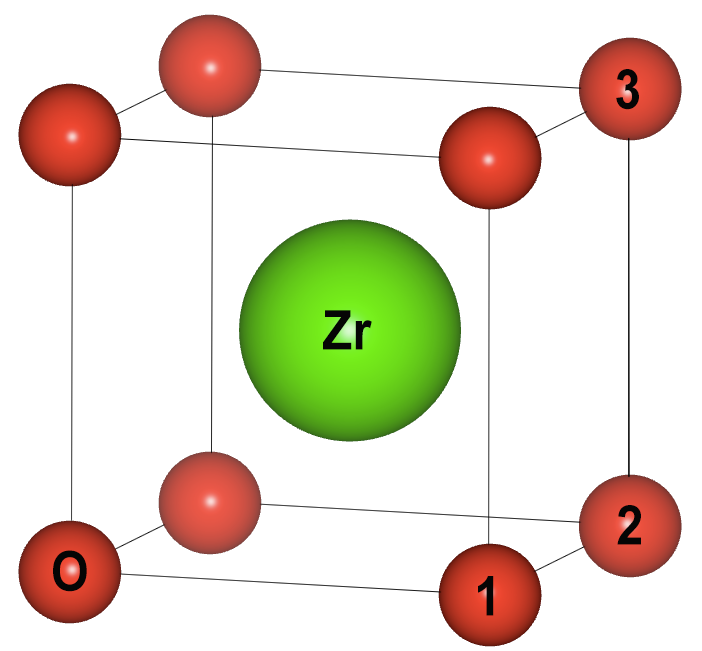
\includegraphics[width=8cm]{images/sd_cubic_zro2.png}
\caption{Zirconium centre showing nearest oxygen atoms in cubic \zirconia. Schottky trios indicated by oxygen enumeration. Zirconium atoms are shown in green and oxygen atoms in red.}
\label{figure:cubicschottky}
\end{figure}

Bound Schottky defects were modelled in a supercell of \zirconia\ by removing one Zr and two O atoms, in one of several possible nearest neighbour configurations as shown in Figures \ref{figure:monoschottky}, \ref{figure:tetschottky} and \ref{figure:cubicschottky}. Charge neutrality is maintained by the removal of a stoichiometric unit, therefore these defects were defined as neutral tri-vacancies (NTVs). The NTV formation energy was defined as:

\begin{equation}
\label{equation_NTV}
E_{NTV} = E_{DFT}(NTV) - \frac{n-3}{n}E_{DFT}(ZrO_2)% - \frac{E_{I_2}}{2}
\end{equation}

Where $E_{DFT}(NTV)$ is the energy of a supercell containing the NTV defect. As the defective supercell contains three fewer ions than the non-defective cell, the energy of the non-defective cell was adjusted by a proportional factor in our calculation. This form maintains both mass and charge balance of the Schottky defect description for \zirconia\ described in Equation \ref{generic_schottky}.

\section{Brouwer diagrams}

\subsection{Defect equilibria}

Typically in materials, several types of defects will exist simultaneously. These defects will be present at an equilibrium concentration based on their thermodynamic stability. There are several considerations to be made. For example, we expect a crystal lattice to be overall charge-neutral, otherwise we would see extreme behaviour at the macro scale which is not indicative of a low-energy state.

\subsection{Oxygen pressure dependence}

The equilibrium concentration of defects will be a function of the oxygen partial pressure, amongst other things like temperature and dopant concentrations. For materials in an equilibrium state, they are necessarily in equilibrium with their surroundings. This is why even metals in evacuated vacuum flasks will produce a metal vapour pressure. In the case of \zirconia\ in nuclear fuel cladding, we know that the ambient oxygen pressure will change over time. In particular, fission of UO$_{2}$ will result in the liberation of oxygen. This will result in an input of gaseous oxygen in the fuel cladding with increasing burn-up. The main oxygen sink is the Zr fuel cladding, into which the oxide grows. Other oxygen sinks include the oxidation of UO$_{2}$ to the ground state oxide U$_{3}$O$_{8}$, and oxidation of fission products. Oxidation of UO$_{2}$ is a slow process whose kinetics are largely independent of the oxygen partial pressure \cite{Desgranges2009}, and will be slowed as free space in the cladding is reduced because it results in swelling of the fuel pellet. 

%\subsection{Brouwer diagram generation} % Good
\chapter{Intrinsic defect study}

\label{ch:results1} % 3

\section{Introduction} % 3.1
\subsection{Applications} % 3.1.1

It is important to fully understand the intrinsic defect structure of \zirconia\ because useful material properties may be exploited to improve performance, e.g. by doping with other ions to stabilise one crystal structure. For example, \zirconia\ doped with enough yttrium cations will stabilise the cubic phase and increase the concentration of oxygen vacancies, which is the main charge carrier in a YSZ solid oxide fuel cell.

\subsection{Crystal structures} % 3.1.2

\zirconia\ grown at standard conditions on Zr metal exists mainly in either the monoclinic or tetragonal phase \cite{Howard1988,teufer1962crystal}. A high temperature cubic phase has also been observed in pure \zirconia , but its similarity to the tetragonal phase often leads to them being mischaracterised in experimental studies. 

\subsection{Previous work} % 3.1.3

Previous works studying intrinsic defects in the \zirconia\ system have utilised quantum mechanical methods to determine defect formation energies in the monoclinic phase \cite{zheng2007first,foster2002modelling,foster2001structure} and defect equilibria in the tetragonal phase \cite{youssef2012intrinsic}. The cubic phase is mainly studied as a dopant-stabilised system \cite{orera1990intrinsic,jiang2011first}, with few undoped defect studies in the literature \cite{mackrodt1986theoretical,aarhammar2009energetics}. Building upon previous quantum mechanical studies, a comprehensive account of intrinsic defect energies, defect volumes, and defect equilibria for all three common crystal structures of \zirconia\ is provided, using state-of-the-art, accessible methods.

\section{Methodology}
\subsection{Simulation parameters}

Density functional theory (DFT) calculations were performed using CASTEP 8.0 \cite{Clark2005}. Ultra-soft pseudo-potentials were used throughout, employing a 600 eV cut-off energy. The Perdew, Burke and Ernzerhof (PBE) \cite{Perdew1996} parameterisation of the generalised gradient approximation (GGA) was used to describe the exchange correlation functional. A Monkhorst-Pack sampling scheme \cite{Monkhorst1976} was used for Brillouin zone integration, with a minimum \emph{k}-point separation of 0.09 \r{A}\textsuperscript{-1}. The Pulay method for density mixing \cite{Pulay1980} was used to improve convergence of simulations. 

The electrical energy convergence criterion was set to $1\times10^{-6} $ eV. The maximum force between atoms was limited to $1\times10^{-2}$ eV \r{A}\textsuperscript{-1}. A gradient-descent geometry optimisation task was run on the cell until consecutive iterations differed in energy and atomic displacement by less than $1\times10^{-5}$ eV and $5\times10^{-4}$ \r{A}, respectively. 


\subsection{Temperature dependence}

To determine the temperature dependence of the ground states for the pure crystal structures, a harmonic approximation method as described by Burr et al. was used \cite{burr2015crystal,jackson2016resolving}. A constant-volume phonon calculation was performed for each structure, from which the vibrational enthalpy $H_{vib}(T, V)$ and entropy $S_{vib}(T, V)$ contributions to the Helmholtz free energy were calculated up to a temperature of 2500 K. The complete Helmholtz free energy $F(T, V)$ was then obtained by including the internal energy $U(V)$ and configurational entropy $S_{conf}$ of the system:

\begin{equation} \label{helmholtz_equation}
F(T, V) = U(V) + H_{vib}(T, V) - TS_{vib}(T, V) - TS_{conf}
\end{equation}

\subsection{Defect formation energies}

Defective formation energies are calculated using equation \ref{equation:formation_energy}:

\begin{equation} \label{equation:formation_energy}
    E_{f} = E_{def} - E_{perf} + \sum_{i} n_i\mu_i + q(\mu_{e} - E_{VBM}) + E_{corr}
\end{equation}

where $E_{f}$ is the formation energy, $E_{def}$ is the energy of the defective supercell, $E_{perf}$ is the energy of a non-defective supercell, $q$ is the defect charge, $E_{VBM}$ is the valence band maximum, $\mu_{e}$ is the Fermi energy and $E_{corr}$ is a charged-cell correction term.

\subsection{Brouwer diagrams}

Brouwer diagrams, also known as Kr{\"o}ger-Vink diagrams, were produced using a method outlined by Murphy et al. \cite{Murphy2014} to determine defect concentrations as a function of oxygen partial pressure. We start from the statement that the chemical potential of \zirconia\ is equivalent to the sum of the chemical potentials $\mu$ of its constituent species, Zr and O:

\begin{equation}
{\mu}_{ZrO_2(s)} = {\mu}_{Zr}(p_{O_2}, T) + {\mu}_{O_2}(p_{O_2}, T)
\label{mewZrO2results1}
\end{equation}

where $T$ denotes temperature and $p_{O_2}$ denotes oxygen partial pressure. The chemical potential of \zirconia\ in the solid state is assumed to have negligible dependence on $T$ and $p_{O_2}$ relative to ${\mu}_{Zr}$ and ${\mu}_{O_2}$. Energies can be obtained for bulk \zirconia\ and Zr, but the ground state of oxygen is not correctly reproduced in DFT \cite{Batyrev2000,Lozovoi2001}. Instead, the approach of Finnis et al. \cite{Finnis2005} is used to infer the oxygen chemical potential from standard state values. Thee experimental Gibbs free energy can be used to produce an equation where $\mu_{O_2}$ is the only unknown:

\begin{equation}
\Delta{G^{\plimsoll}_{f, ZrO_2}} = \mu_{ZrO_2(s)} - (\mu_{Zr(s)} + \mu^{\plimsoll}_{O_2})
\end{equation}

where $\Delta{G^{\plimsoll}_{f, ZrO_2}}$ is the experimental Gibbs energy at standard temperature and pressure and $\mu^{\plimsoll}_{O_2}$ is the oxygen chemical potential under the same conditions. The values of $\mu_{ZrO_2(s)}$ and $\mu_{Zr(s)}$ are calculated from the DFT energies. Once $\mu^{\plimsoll}_{O_2}$ is calculated, chemical potential of oxygen is generalised for any value of $T$ and $p_{O_2}$ by appending an ideal gas relationship $\Delta{\mu(T)}$ and a Boltzmann distribution:

\begin{equation}
\mu_{O_2}(p_{O_2},T) = \mu^{\plimsoll}_{O_2} + \Delta{\mu(T)} + \frac{1}{2}{k_B}log(\frac{p_{O_2}}{p^{\plimsoll}_{O_2}})
\end{equation}

Using our generalised formula for $\mu_{O_2}$, the temperature is fixed within the range of thermal phase-stabilisation (1500 K for tetragonal \zirconia) and calculate $\mu_{O_2}$ for many different values of $p_{O_2}$ between $10^{-35}$ and 10$^{0}$ atm, corresponding to oxygen deficient and oxygen rich environments, respectively ($p_{O_2}$ in air is approximately 0.2 atm). While the tetragonal phase will be stress-stabilised in practice, thermal-stabilisation in such models has been shown to qualitatively approximate the effect of stress-stabilisation, while allowing a wider range of dopant behaviours to be predicted \cite{Bell2016}. Equilibrium defect concentrations are then calculated at each $\mu_{O_2}$ and plotted against $p_{O_2}$ to produce a Brouwer diagram. 

\section{Cubic phase collapse}

\begin{itemize}
\item When some oxygen Frenkel defects were introduced to the cubic phase supercell, relaxation under constant volume conditions caused a collapse into a pseudo-tetragonal structure.
\item This indicated that the cubic phase as modelled in DFT may not be fully stable.
\item Further investigation indicated that the structure of a supercell of c-\zirconia\ broke down even with constrained symmetry, a result corroborated by Burr et al. \cite{burr2017importance}. 
\end{itemize}

\subsection{Electronic density of states}

\begin{figure}
\begin{center}
\begin{tikzpicture}
	\begin{axis}
		[width=\linewidth*0.7, xlabel={Energy (eV)}, ylabel={Electronic density of states}, ymin=0, ymax=12, xmin=0, xmax=16, legend style={{draw=}, at={(0.05,0.95)}, anchor=north west, legend columns=1}]
       \addplot[no marks] table [x=mono_x, y=mono_y,]{dat/eDOS.dat}; \addlegendentry{Monoclinic};
       \addplot[no marks, dashed] table [x=tet_x, y=tet_y,]{dat/eDOS.dat}; \addlegendentry{Tetragonal};
       \addplot[no marks, densely dotted] table [x=cubic_x, y=cubic_y,]{dat/eDOS.dat}; \addlegendentry{Cubic};

			\end{axis}
		\end{tikzpicture}
		\caption{Electronic density of states for the different crystal structures of \zirconia\ showing the band gap predicted by DFT.}
		\label{figure:densityofstates}
	\end{center}
\end{figure}

\begin{table}[htp] % Band Gap
\onehalfspacing
\centering
\caption[Experimentally determined band gaps alongside values calculated from DFT simulations for each crystal structure of zirconia.]{Experimentally determined band gaps alongside values calculated from DFT simulations for each crystal structure of zirconia. Experimental values taken from \cite{French1994}.}
\begin{tabular}{ccc}
{\bf }                                       & \multicolumn{2}{c}{{\bf Band gap (eV)}}      \\ \hline
\multicolumn{1}{c}{{\bf Crystal Structure}} & \multicolumn{1}{c}{{\bf Expt.}} & {\bf DFT} \\ \hline
\multicolumn{1}{c}{Monoclinic}              & \multicolumn{1}{c}{5.83}        & 3.45      \\
\multicolumn{1}{c}{Tetragonal}              & \multicolumn{1}{c}{5.78}        & 4.00      \\
\multicolumn{1}{c}{Cubic}                   & \multicolumn{1}{c}{6.10}         &   3.55 \\ \hline
\label{table:bandgap}
\end{tabular}
\end{table}

\section{Defect formation energies}

\begin{figure}[htp]
\begin{center}
\begin{tikzpicture}
	\begin{axis}
		[width=11cm, xlabel={Fermi level (eV)}, ylabel={Formation energy (eV) per \zirconia\ }, ymin=-10, ymax=18, xmin=0, xmax=6, legend style={{draw=}, at={(0.95,0.95)}, anchor=north east, legend columns=1}]
		\addplot[no marks, blue] table [x=ZRmono1, y=ZRmono2,]{dat/vacancies.dat}; \addlegendentry{Zr};
        \addplot[no marks, red, dashed] table [x=O3mono1, y=O3mono2,]{dat/vacancies.dat}; \addlegendentry{O (III)};
        \addplot[no marks, red] table [x=O4mono1, y=O4mono2,]{dat/vacancies.dat}; \addlegendentry{O (IV)};
			\end{axis}
		\end{tikzpicture}
		\caption{Monoclinic phase formation energies of intrinsic vacancy defects as a function of Fermi level. Gradient indicates defect charge. Oxygen coordination number shown in legend.}
		\label{figure:monovacancies}
	\end{center}
\end{figure}


\begin{figure}[htp]
\begin{center}
\begin{tikzpicture}
	\begin{axis}
		[width=11cm, xlabel={Fermi level (eV)}, ylabel={Formation energy (eV) per \zirconia\ }, ymin=-10, ymax=18, xmin=0, xmax=6, legend style={{draw=}, at={(0.95,0.95)}, anchor=north east, legend columns=1}]
		\addplot[no marks, blue] table [x=ZRtet1, y=ZRtet2,]{dat/vacancies.dat}; \addlegendentry{Zr};
        \addplot[no marks, red] table [x=Otet1, y=Otet2,]{dat/vacancies.dat}; \addlegendentry{O};
			\end{axis}
		\end{tikzpicture}
		\caption{Tetragonal phase formation energies of intrinsic vacancy defects as a function of Fermi level. Gradient indicates defect charge.}
		\label{figure:tetvacancies}
	\end{center}
\end{figure}

\begin{figure}[htp]
\begin{center}
\begin{tikzpicture}
	\begin{axis}
		[width=11cm, xlabel={Fermi level (eV)}, ylabel={Formation energy (eV) per \zirconia\ }, ymin=-10, ymax=18, xmin=0, xmax=6, legend style={{draw=}, at={(0.95,0.95)}, anchor=north east, legend columns=1}]
		\addplot[no marks, blue] table [x=ZRcubic1, y=ZRcubic2,]{dat/vacancies.dat}; \addlegendentry{Zr};
        \addplot[no marks, red] table [x=Ocubic1, y=Ocubic2,]{dat/vacancies.dat}; \addlegendentry{O};
			\end{axis}
		\end{tikzpicture}
		\caption{Cubic phase formation energies of intrinsic vacancy defects as a function of Fermi level. Gradient indicates defect charge.}
		\label{figure:cubicvacancies}
	\end{center}
\end{figure}

\begin{figure}[htp]
\begin{center}
\begin{tikzpicture}
	\begin{axis}
		[width=11.5cm, xlabel={Fermi level (eV)}, ylabel={Formation energy (eV) per \zirconia\ }, ymin=4, ymax=11, xmin=0, xmax=6, legend style={{draw=}, at={(0.5,0.05)}, anchor=south, legend columns=2}]
		\addplot[no marks, red] table [x=2a1, y=2a2,]{dat/monointer.dat}; \addlegendentry{$2a\overline{1}$};
        \addplot[no marks, red, dashed] table [x=2b1, y=2b2, ]{dat/monointer.dat}; \addlegendentry{$2b\overline{1}$};
        \addplot[no marks, blue] table [x=2c1, y=2c2,]{dat/monointer.dat}; \addlegendentry{$2c\overline{1}$};
        \addplot[no marks, blue, dashed] table [x=2d1, y=2d2,]{dat/monointer.dat}; \addlegendentry{$2d\overline{1}$};
			\end{axis}
		\end{tikzpicture}
		\caption{Monoclinic phase formation energies of iodine interstitial defects as a function of Fermi level. Gradient indicates defect charge.}
		\label{figure:monointer}
	\end{center}
\end{figure}


\begin{figure}[htp]
\begin{center}
\begin{tikzpicture}
	\begin{axis}
		[width=11cm, xlabel={Fermi level (eV)}, ylabel={Formation energy (eV) per \zirconia\ }, ymin=6, ymax=11, xmin=0, xmax=6, legend style={{draw=}, at={(0.5,0.05)}, anchor=south, legend columns=1}]
		\addplot[no marks, red] table [x=2atet1, y=2atet2,]{dat/tetcubicinter.dat}; \addlegendentry{$2a\overline{4}m2$};
        \addplot[no marks, blue] table [x=8etet1, y=8etet2, ]{dat/tetcubicinter.dat}; \addlegendentry{$8e\overline{1}$};
			\end{axis}
		\end{tikzpicture}
		\caption{Tetragonal phase formation energies of iodine interstitial defects as a function of Fermi level. Gradient indicates defect charge.}
		\label{figure:tetinter}
	\end{center}
\end{figure}

\begin{figure}[htp]
\begin{center}
\begin{tikzpicture}
	\begin{axis}
		[width=11cm, xlabel={Fermi level (eV)}, ylabel={Formation energy (eV) per \zirconia\ }, ymin=8, ymax=13, xmin=0, xmax=6, legend style={{draw=}, at={(0.5,0.05)}, anchor=south, legend columns=1}]
		\addplot[no marks, red] table [x=24cubic1, y=24cubic2,]{dat/tetcubicinter.dat}; \addlegendentry{$24dm.mm$};
        \addplot[no marks, blue] table [x=4bmcubic1, y=4bmcubic2, ]{dat/tetcubicinter.dat}; \addlegendentry{$4bm\overline{3}m$};
			\end{axis}
		\end{tikzpicture}
		\caption{Cubic phase formation energies of iodine interstitial defects as a function of Fermi level. Gradient indicates defect charge.}
		\label{figure:cubicinter}
	\end{center}
\end{figure}

Defect volumes of isolated Frenkel defects can be seen in Table \ref{defect_volumes_clusters_isolated}.


\subsection{Defect Volumes}

Tables \ref{defect_volumes_raw} and \ref{defect_volumes_clusters_isolated} show the calculated point defect and cluster defect volumes respectively. The Frenkel and Schottky defect volumes are calculated from the sum of the relevant point defects that would result in an overall neutral charge, with clusters of fully-charged point defects being the expected defect structures in a real material.

The oxygen Frenkel defect has the smallest defect volume in the monoclinic phase, followed by the tetragonal phase. This can be explained by the competition between phase density and matrix stiffness. As the monoclinic phase has the highest specific volume (see Table \ref{lattice_params}), we can argue that the monoclinic phase can best absorb the lattice strains imposed by the defect, despite having a lower stiffness than the cubic phase.

The zirconium Frenkel defect is significantly larger than the oxygen Frenkel, mostly due to the large positive strain contribution from the zirconium vacancy. This can explain the larger defect formation energy of zirconium Frenkels.

\begin{table}[htp] % Isolated Frenkel volumes
\onehalfspacing
\centering
\caption{Isolated cluster defect volumes in the three \zirconia\ structures.}
\label{defect_volumes_clusters_isolated}
\begin{tabular}{cccc}
\hline
                      & \multicolumn{3}{c}{\textbf{Relaxation Volume (\r{A}\textsuperscript{3})}}  \\ \cline{2-4} 
\textbf{Defect}       & \textbf{Monoclinic} & \textbf{Tetragonal} & \textbf{Cubic} \\ \hline
\ch{V_{Zr}^{''''}} + \ch{Zr_{i}^{****}}          & 21.331	 & 25.4702 &	21.1309         \\
\ch{V_{Zr}^{'''}} + \ch{Zr_{i}^{***}}          & 19.7155 &	23.3463 &	19.9954      \\
\ch{V_{Zr}^{''}} + \ch{Zr_{i}^{**}}          & 18.1149 &	22.2525 &	19.68618           \\
\ch{V_{Zr}^{'}} + \ch{Zr_{i}^{*}}          & 19.78339 &	18.4096913 &	19.76396           \\
\ch{V_{Zr}^{x}} + \ch{Zr_{i}^{x}}          & 19.99485 &	18.1061 &	20.29223       \\
\ch{V_{O}^{**}} + \ch{O_{i}^{''}}           & 0.8839 &	2.4704 &	5.8217       \\
\ch{V_{O}^{*}} + \ch{O_{i}^{'}}           &  0.9486 &	5.032 &	4.1146        \\
\ch{V_{O}^{x}} + \ch{O_{i}^{x}}           &  0.9576 &	8.26065 &	7.83687          \\
\ch{V_{Zr}^{''''}} + 2\ch{V_{O}^{**}}       &  3.6979 &	-7.647 &	2.9448             \\
\ch{V_{Zr}^{''}} + 2\ch{V_{O}^{*}}       &  1.0707 &	-4.7866 &	1.5564         \\
\ch{V_{Zr}^{x}} + 2\ch{V_{O}^{x}}        & 0.64517 &	-0.8985 &	2.08973       \\ \hline
\end{tabular}
\end{table}

\subsubsection*{Isolated Defects}

The isolated defect formation energies reported in Table \ref{isolated_defects} indicate that fully-charged Schottky defects have the lowest formation energy per atom (most energetically favourable) in all phases, followed by oxygen Frenkel defects. A trend is seen where the high-temperature phases result in lower formation energies for both Schottky and oxygen Frenkel defects, whereas zirconium Frenkel defects have similar formation energies in all three phases. It has been suggested that the relatively small cation size leads to defect structures where oxygen vacancies are favoured over interstitial defects \cite{dwivedi1990computer}. As the zirconium ion is too small to maintain a strong 8-fold bond coordination with its neighbouring oxygen ions, the introduction of oxygen vacancies (which have the added effect of reducing cell volume) will have a stabilising effect.

\begin{table}[htp] % Isolated formation energies
\onehalfspacing
\centering
\caption{Formation energies in eV of isolated \zirconia\ defects.}
\label{isolated_defects}
\begin{tabular}{cccll}
\hline
\multirow{2}{*}{\textbf{Defect}}                      & \multirow{2}{*}{\textbf{Equation}}                                        & \multicolumn{3}{c}{\textbf{Formation Energy (eV)}} \\ \cline{3-5}
	&	& \multicolumn{1}{l}{Monoclinic} & Tetragonal & Cubic \\ \hline
\multirow{5}{*}{\textbf{Zr Frenkel}} & \ch{Zr_{Zr}^{x}} $\rightarrow$ \ch{V_{Zr}^{''''}} + \ch{Zr_{i}^{****}}              & 5.428 & 5.639 & 5.610                             \\
                                     & \ch{Zr_{Zr}^{x}} $\rightarrow$ \ch{V_{Zr}^{'''}} + \ch{Zr_{i}^{***}}               & 8.695 & 8.939 & 8.476                            \\
                                     & \ch{Zr_{Zr}^{x}} $\rightarrow$ \ch{V_{Zr}^{''}} + \ch{Zr_{i}^{**}}                & 12.118 & 12.058 & 11.628                             \\
                                     & \ch{Zr_{Zr}^{x}} $\rightarrow$ \ch{V_{Zr}^{'}} + \ch{Zr_{i}^{*}}                & 16.021 &	15.696 &	13.319                             \\
                                     & \ch{Zr_{Zr}^{x}} $\rightarrow$ \ch{V_{Zr}^{x}} + \ch{Zr_{i}^{x}}                  & 20.563	& 20.094 &	18.170                            \\ \hline
\multirow{3}{*}{\textbf{O Frenkel}}  & \ch{O_{O}^{x}} $\rightarrow$ \ch{V_{O}^{**}} + \ch{O_{i}^{''}}                   & 4.457 &	4.000 & 	3.728                             \\
                                     & \ch{O_{O}^{x}} $\rightarrow$ \ch{V_{O}^{*}} + \ch{O_{i}^{'}}                   & 6.432	& 6.588 &	7.055                             \\
                                     & \ch{O_{O}^{x}} $\rightarrow$ \ch{V_{O}^{x}} + \ch{O_{i}^{x}}                     & 7.518 &	7.452 &	8.477                             \\ \hline
\multirow{3}{*}{\textbf{Schottky}}   & $\varnothing$ $\rightarrow$ \ch{V_{Zr}^{''''}} + 2\ch{V_{O}^{**}} & 5.120 &	3.778	& 1.752                             \\
                                     & $\varnothing$ $\rightarrow$ \ch{V_{Zr}^{''}} + 2\ch{V_{O}^{*}} & 11.353 &	10.832 &	9.624                             \\
                                     & $\varnothing$ $\rightarrow$ \ch{V_{Zr}^{x}} + 2\ch{V_{O}^{x}}   & 18.554 &	18.232 &	17.073  \\ \hline                          
\end{tabular}
\end{table}

\subsubsection*{Bound Defects}
The bound defect formation energies shown in Table \ref{table:bound_defects} show that NTV defects, on a per defect atom basis, are the most energetically favourable defects, followed by oxygen and zirconium Frenkel defects respectively. The NTV3 exhibited the smallest formation energy in all three crystal structure, with a single exception of the NTV2 in the cubic phase where a much smaller formation energy was observed due to collapse of the supercell during geometry optimisation.

\begin{table}[htp] % Bound formation energies
\onehalfspacing
\centering
\caption{Formation energies of bound defects in \zirconia.}
\label{table:bound_defects}
\begin{tabular}{cccc}
\hline
\multirow{2}{*}{\textbf{Defect}} & \multicolumn{3}{c}{\textbf{Formation Energy (eV)}} \\ \cline{2-4} 
 & \textbf{Monoclinic} & \textbf{Tetragonal} & \textbf{Cubic} \\ \hline
\textbf{O Frenkel} & 4.1212 & 4.0290 & 6.4397 \\
\textbf{Zr Frenkel} & 8.4232 & 7.8633 & 6.3274 \\
\textbf{NTV1} & 5.2272 & 3.5813 & 2.6961 \\
\textbf{NTV2} & 5.1405 & 4.2312 & 0.1798 \\
\textbf{NTV3} & 4.6620 & 3.3623 & 2.4089 \\ \hline
\end{tabular}
\end{table}

\section{Elastic constants and defect relaxation volumes}

Table \ref{stiffness_tensor} shows the calculated elastic constants for the monoclinic, tetragonal, and cubic phases of \zirconia . The cubic phase has the highest stiffness, likely due to the short Zr-O bond lengths in the energy-minimised structure (Figure \ref{figure:zrobonddistance}). It is expected that at high temperatures where the cubic phase is stable, the resulting increase in bond length would cause a reduction in stiffness. 

The monoclinic and tetragonal phases have similar stiffness along the principal axes, but vary significantly under shearing conditions. In particular, the tetragonal phase exhibits much smaller $C_{44}$ and $C_{55}$ components. This may be attributed to the strong directional anisotropy of the tetragonal phase due to the larger $c$ parameter. 


\begin{table}[htp] % Elastic constants
\onehalfspacing
\centering
\caption{Elastic constants for different phases of \zirconia\ from DFT calculations.}
\label{stiffness_tensor}
\begin{tabular}{cccc}
\hline
\multirow{2}{*}{\textbf{Elastic Component}} & \multicolumn{3}{c}{\textbf{Stiffness (GPa)}}               \\ \cline{2-4} 
                                            & \textbf{Monoclinic} & \textbf{Tetragonal} & \textbf{Cubic} \\ \hline
$C_{11}$                                         & 338.86        & 334.30               & 523.38    \\
$C_{12}$                                         & 151.80        & 207.30               & 92.93     \\
$C_{13}$                                         & 89.37         & 48.93               & 92.93     \\
$C_{22}$                                         & 348.37        & 334.20               & 523.39    \\
$C_{23}$                                         & 143.04        & 48.93               & 92.93    \\
$C_{33}$                                         & 262.17        & 250.50               & 523.38   \\
$C_{44}$                                         & 76.35         & 9.38                & 61.98    \\
$C_{55}$                                         & 71.65         & 9.38                & 61.98   \\
$C_{66}$                                         & 114.19        & 152.60               & 61.99     \\ \hline
\end{tabular}
\end{table}

\begin{table}[htp] % Isolated defect volumes
\onehalfspacing
\centering
\caption{Isolated defect volumes in the three \zirconia\ structures.}
\label{defect_volumes_raw}
\begin{tabular}{cccc}
\hline
                      & \multicolumn{3}{c}{\textbf{Volume (\r{A}\textsuperscript{3})}}  \\ \cline{2-4} 
\textbf{Defect}       & \textbf{Monoclinic} & \textbf{Tetragonal} & \textbf{Cubic} \\ \hline
\ch{V_{Zr}^{''''}}             & 55.9495             & 67.4062             & 48.468         \\
\ch{V_{Zr}^{'''}}             & 42.4752             &         51.0824     &     36.944      \\
\ch{V_{Zr}^{''}}            & 29.9013             &  34.2764            &     25.9264           \\
\ch{V_{Zr}^{'}}             & 17.1031             &  18.4276            &     15.0761           \\
\ch{V_{Zr}^{x}}              & 4.05915             &  4.70160            &    4.31893       \\
\ch{Zr_{i}^{****}}             & -34.6185            & -41.936             & -27.3371       \\
\ch{Zr_{i}^{***}}             &  -22.7597           &	-27.7361 		  &	-16.9486         \\
\ch{Zr_{i}^{**}}             &  -11.7864 	        &	-12.0239 		  &	-6.24022          \\
\ch{Zr_{i}^{*}}            &  2.68029			& -0.0179087 		  & 	4.68786             \\
\ch{Zr_{i}^{x}}              &  15.9357		 	& 13.4045	 		  & 15.9733         \\
\ch{V_{O}^{**}} {[}4coord{]} & -22.5154            & -37.5266            & -22.7616       \\
\ch{V_{O}^{*}} {[}4coord{]} &  -12.4114           &    -19.5315         &     -12.1850           \\
\ch{V_{O}^{x}} {[}4coord{]}  &  -0.686074          &  -2.80005           &      -1.1146          \\
\ch{V_{O}^{**}} {[}3coord{]} & -26.1258            &                     &                \\
\ch{V_{O}^{*}} {[}3coord{]} &  -14.4153           &                     &                \\
\ch{V_{O}^{x}} {[}3coord{]}  &   -1.70699          &                     &                \\
\ch{O_{i}^{''}}              & 27.0097             & 39.997              & 28.5833        \\
\ch{O_{i}^{'}}              &  15.3639            &    24.5635          &  16.2996              \\
\ch{O_{i}^{x}}               & 2.66459             &    11.0607          &   8.95147        \\ \hline
\end{tabular}
\end{table}

\section{Helmholtz energies}

%The calculated Helmholtz energies plotted in Figure \ref{Figure:helmholtz} show the correct order of stability for the three phases of \zirconia\ at low temperatures (monoclinic $\rightarrow$ tetragonal $\rightarrow$ cubic) . However, as temperature is increased, only a transition from monoclinic to tetragonal is seen. The cubic phase Helmholtz energy does fall below the monoclinic curve, but never below the tetragonal curve, thus predicting no tetragonal to cubic phase transition. 

%It must also be noted that the transition temperatures are not predicted accurately. The tetragonal phase is predicted to have a lower energy than monoclinic at approximately 400 K, while experiments indicate that the transition temperature is above 1400 K. This difference is too large to attribute to a kinetic barrier.

The Helmholtz free energy results (Figure \ref{Figure:helmholtz}) show the correct order of crystal structure stability at low temperature. A transition from the monoclinic to tetragonal crystal structure is seen at 390K, but no further transition is seen from tetragonal to cubic. The low monoclinic-tetragonal transition temperature may be due to both the kinetic barrier \cite{bansal1972martensitic,bansal1974martensitic}, and the inability of the constant volume harmonic model to take into account the effects of thermal expansion. The lack of an observed transition to the cubic phase may indicate an inability to accurately simulate the high-temperature phase using DFT techniques. 


\begin{figure}[ht] % Helmholtz
\begin{center}
\begin{tikzpicture}
	\begin{axis}
		[width=\linewidth*0.7, xlabel={Temperature (K)}, ylabel={Helmholtz free energy (eV)}, ymin=-28, ymax=-10, xmin=0, xmax=3000, legend style={{draw=}, at={(0.95,0.95)}, anchor=north east, legend columns=1}]
		\addplot[no marks] table [x=temperature, y=monoclinic,]{dat/helmholtz.dat}; \addlegendentry{Monoclinic};
        \addplot[no marks, dashed] table [x=temperature, y=tetragonal, ]{dat/helmholtz.dat}; \addlegendentry{Tetragonal};
        \addplot[no marks, densely dotted, black] table [x=temperature, y=cubic,]{dat/helmholtz.dat}; \addlegendentry{Cubic};
			\end{axis}
		\end{tikzpicture}
		\caption{Helmholtz free energy as a function of temperature for the monoclinic, tetragonal, and cubic crystal structures of \zirconia .}
		\label{Figure:helmholtz}
	\end{center}
\end{figure}

\section{Defect equilibria}

\subsubsection*{Monoclinic}

The monoclinic Brouwer diagram (Figure \ref{figure:mono_intrinsic_brouwer}) predicts that at 635 K, few types of defects will be present and at very low (\textless 10 ppb \zirconia ) concentrations. This is typical of defect behaviour in a ceramics at temperatures far below their melting points \cite{kingery1997physical,ball2006computer}. Fully-charged zirconium vacancies, charge-compensated by holes, are the major defect type we expect to observe at $p_{O_{2}}$ \textgreater $10^{-15}$ atm. Below this, only electronic defects compensated by electron hole defects are expected. 

%We briefly see increased concentrations of uncharged oxygen interstitial defects at very high levels of $p_{O_{2}}$.
%The intrinsic defect equilibria are shown in Brouwer diagrams in Figures \ref{figure:mono_intrinsic_brouwer}, \ref{figure:tet_intrinsic_brouwer} and \ref{figure:cubic_intrinsic_brouwer}. The monoclinic phase exhibits the smallest overall concentration of intrinsic defects due to the low temperature (650 K) relative to the other tetragonal (1500 K) and cubic (XXX K) phases.

\begin{figure}[ht] % Mono intrinsic Brouwer
\begin{center}
\begin{tikzpicture}
	\begin{axis}
		[width=\linewidth*0.7, xlabel={\ch{log_{10}}($p_{O_{2}}$) (atm)}, ylabel={\ch{log_{10}}([D]) (per f.u.)}, ymin=-18, ymax=0, xmin=-35, xmax=0, legend style={{draw=}, at={(0.40,0.94)}, anchor=north west, legend columns=4, nodes={scale=1, transform shape}}]
        \addplot[no marks, draw=blue!70!black] table [x=pO2, y=electrons,]{dat/intrinsic_mono.dat}; \addlegendentry{\ch{e^{'}}}; \node at (-4.8,-13) {\ch{e^{'}}};
        \addplot[no marks, draw=red!85!black] table [x=pO2, y=holes,]{dat/intrinsic_mono.dat}; \addlegendentry{\ch{h^{\textperiodcentered}}}; \node at (-4.5,-8) {\ch{h^{\textperiodcentered}}};
        \addplot[no marks, draw=black!70!green] table [x=pO2, y=VO{2},]{dat/intrinsic_mono.dat}; \addlegendentry{\ch{V_{O}^{\textperiodcentered\textperiodcentered}}}; \node at (-33,-16.5) {\ch{V_{O}^{\textperiodcentered\textperiodcentered}}};
%         \addplot[no marks, draw=black!55!green] table [x=pO2, y=VO{1},]{dat/intrinsic_mono.dat}; \addlegendentry{\ch{V_{O}^{*}}};
%         \addplot[no marks, draw=black!30!green] table [x=pO2, y=VO{0},]{dat/intrinsic_mono.dat}; \addlegendentry{\ch{V_{O}^{x}}};
        \addplot[no marks, draw=yellow!85!blue] table [x=pO2, y=VM{-4},]{dat/intrinsic_mono.dat}; \addlegendentry{\ch{V_{Zr}^{''''}}}; \node at (-5,-10.5) {\ch{V_{Zr}^{''''}}};
%         \addplot[no marks, draw=yellow!75!blue] table [x=pO2, y=VM{-3},]{dat/intrinsic_mono.dat}; \addlegendentry{\ch{V_{Zr}^{'''}}};
%         \addplot[no marks, draw=yellow!65!blue] table [x=pO2, y=VM{-2},]{dat/intrinsic_mono.dat}; \addlegendentry{\ch{V_{Zr}^{''}}};
%         \addplot[no marks, draw=yellow!55!blue] table [x=pO2, y=VM{-1},]{dat/intrinsic_mono.dat}; \addlegendentry{\ch{V_{Zr}^{'}}};
%         \addplot[no marks, draw=yellow!45!blue] table [x=pO2, y=VM{0},]{dat/intrinsic_mono.dat}; \addlegendentry{\ch{V_{Zr}^{x}}};
%         \addplot[no marks, draw=red!60!yellow] table [x=pO2, y=Oi{-2},]{dat/intrinsic_mono.dat}; \addlegendentry{\ch{O_{i}^{''}}};
%         \addplot[no marks, draw=red!50!yellow] table [x=pO2, y=Oi{-1},]{dat/intrinsic_mono.dat}; \addlegendentry{\ch{O_{i}^{'}}};
%         \addplot[no marks, draw=red!40!yellow] table [x=pO2, y=Oi{0},]{dat/intrinsic_mono.dat}; \addlegendentry{\ch{O_{i}^{x}}};
%         \addplot[no marks, draw=green!80!pink] table [x=pO2, y=Mi{4},]{dat/intrinsic_mono.dat}; \addlegendentry{\ch{Zr_{i}^{****}}};
%         \addplot[no marks, draw=green!70!pink] table [x=pO2, y=Mi{3},]{dat/intrinsic_mono.dat}; \addlegendentry{\ch{Zr_{i}^{***}}};
%         \addplot[no marks, draw=green!60!pink] table [x=pO2, y=Mi{2},]{dat/intrinsic_mono.dat}; \addlegendentry{\ch{Zr_{i}^{\textbf{**}}}};
%         \addplot[no marks, draw=green!50!pink] table [x=pO2, y=Mi{1},]{dat/intrinsic_mono.dat}; \addlegendentry{\ch{Zr_{i}^{*}}};
%         \addplot[no marks, draw=green!40!pink] table [x=pO2, y=Mi{0},]{dat/intrinsic_mono.dat}; \addlegendentry{\ch{Zr_{i}^{x}}};
%         \addplot[no marks] table [x=pO2, y=Stoich,]{dat/intrinsic_mono.dat}; \addlegendentry{Stoich};
%\node at (-33.7,-0.5) {\textbf{a)}};
			\end{axis}            
\end{tikzpicture}
		\caption{Monoclinic phase Brouwer diagram of intrinsic defects at 650 K.}
		\label{figure:mono_intrinsic_brouwer}
	\end{center}
\end{figure}


\subsubsection*{Tetragonal}

Figure \ref{figure:tet_intrinsic_brouwer} shows a much greater concentration of defects across a wide range of $p_{O_{2}}$, mainly owing to an elevated temperature of 1500 K where the tetragonal crystal structure is fully stabilised. At low levels of $p_{O_{2}}$, electronic defects are again the dominant defect, but are now charge-compensated by the formation of fully-charged oxygen vacancies. A clear neutrality condition is seen at a $p_{O_{2}}$ of $10^{-11}$ atm where $[\ch{V_{O}^{**}}] = 2[\ch{V_{Zr}^{''''}}]$, with higher levels of $p_{O_{2}}$ being dominated by fully-charged zirconium vacancies charge-compensated by the formation of electron hole defects.

\begin{figure}[ht] % Tet intrinsic Brouwer
\begin{center}
\begin{tikzpicture}
	\begin{axis}
		[width=\linewidth*0.7, xlabel={\ch{log_{10}}($p_{O_{2}}$) (atm)}, ylabel={\ch{log_{10}}([D]) (per f.u.)}, ymin=-10, ymax=0, xmin=-35, xmax=0, legend style={{draw=}, at={(0.40,0.97)}, anchor=north west, legend columns=4, nodes={scale=1, transform shape}}]
        \addplot[no marks, draw=blue!70!black] table [x=pO2, y=electrons,]{dat/intrinsic_tet.dat}; \addlegendentry{\ch{e^{'}}}; \node at (-26.0,-2) {\ch{e^{'}}};
        \addplot[no marks, draw=red!85!black] table [x=pO2, y=holes,]{dat/intrinsic_tet.dat}; \addlegendentry{\ch{h^{\textperiodcentered}}}; \node at (-7,-3.6) {\ch{h^{\textperiodcentered}}};
        \addplot[no marks, draw=black!70!green] table [x=pO2, y=VO{2},]{dat/intrinsic_tet.dat}; \addlegendentry{\ch{V_{O}^{\textperiodcentered\textperiodcentered}}}; \node at (-28,-3) {\ch{V_{O}^{\textperiodcentered\textperiodcentered}}};
%         \addplot[no marks, draw=black!55!green] table [x=pO2, y=VO{1},]{dat/intrinsic_tet.dat}; \addlegendentry{\ch{V_{O}^{*}}};
%         \addplot[no marks, draw=black!30!green] table [x=pO2, y=VO{0},]{dat/intrinsic_tet.dat}; \addlegendentry{\ch{V_{O}^{x}}};
        \addplot[no marks, draw=yellow!85!blue] table [x=pO2, y=VM{-4},]{dat/intrinsic_tet.dat}; \addlegendentry{\ch{V_{Zr}^{''''}}}; \node at (-3,-4.5) {\ch{V_{Zr}^{''''}}};
%         \addplot[no marks, draw=yellow!75!blue] table [x=pO2, y=VM{-3},]{dat/intrinsic_tet.dat}; \addlegendentry{\ch{V_{Zr}^{'''}}};
%         \addplot[no marks, draw=yellow!65!blue] table [x=pO2, y=VM{-2},]{dat/intrinsic_tet.dat}; \addlegendentry{\ch{V_{Zr}^{''}}};
%         \addplot[no marks, draw=yellow!55!blue] table [x=pO2, y=VM{-1},]{dat/intrinsic_tet.dat}; \addlegendentry{\ch{V_{Zr}^{'}}};
%         \addplot[no marks, draw=yellow!45!blue] table [x=pO2, y=VM{0},]{dat/intrinsic_tet.dat}; \addlegendentry{\ch{V_{Zr}^{x}}};
%         \addplot[no marks, draw=red!60!yellow] table [x=pO2, y=Oi{-2},]{dat/intrinsic_tet.dat}; \addlegendentry{\ch{O_{i}^{''}}};
%         \addplot[no marks, draw=red!50!yellow] table [x=pO2, y=Oi{-1},]{dat/intrinsic_tet.dat}; \addlegendentry{\ch{O_{i}^{'}}};
%         \addplot[no marks, draw=red!40!yellow] table [x=pO2, y=Oi{0},]{dat/intrinsic_tet.dat}; \addlegendentry{\ch{O_{i}^{x}}};
%         \addplot[no marks, draw=green!80!pink] table [x=pO2, y=Mi{4},]{dat/intrinsic_tet.dat}; \addlegendentry{\ch{Zr_{i}^{****}}};
%         \addplot[no marks, draw=green!70!pink] table [x=pO2, y=Mi{3},]{dat/intrinsic_tet.dat}; \addlegendentry{\ch{Zr_{i}^{***}}};
%         \addplot[no marks, draw=green!60!pink] table [x=pO2, y=Mi{2},]{dat/intrinsic_tet.dat}; \addlegendentry{\ch{Zr_{i}^{\textbf{**}}}};
%         \addplot[no marks, draw=green!50!pink] table [x=pO2, y=Mi{1},]{dat/intrinsic_tet.dat}; \addlegendentry{\ch{Zr_{i}^{*}}};
%         \addplot[no marks, draw=green!40!pink] table [x=pO2, y=Mi{0},]{dat/intrinsic_tet.dat}; \addlegendentry{\ch{Zr_{i}^{x}}};
%         \addplot[no marks] table [x=pO2, y=Stoich,]{dat/intrinsic_tet.dat}; \addlegendentry{Stoich};
%\node at (-33.7,-0.5) {\textbf{a)}};
			\end{axis}            
\end{tikzpicture}
		\caption{Tetragonal phase Brouwer diagrams of intrinsic defects at 1500 K.}
		\label{figure:tet_intrinsic_brouwer}
	\end{center}
\end{figure}

\begin{figure}[ht] % cubic intrinsic Brouwer
\begin{center}
\begin{tikzpicture}
	\begin{axis}
		[width=\linewidth*0.7, xlabel={\ch{log_{10}}($p_{O_{2}}$) (atm)}, ylabel={\ch{log_{10}}([D]) (per f.u.)}, ymin=-10, ymax=0, xmin=-35, xmax=0, legend style={{draw=}, at={(0.60,0.97)}, anchor=north west, legend columns=3, nodes={scale=1, transform shape}}]
        \addplot[no marks, draw=blue!70!black] table [x=pO2, y=electrons,]{dat/intrinsic_cubic.dat}; \addlegendentry{\ch{e^{'}}}; \node at (-17.0,-1) {\ch{e^{'}}};
        \addplot[no marks, draw=red!85!black] table [x=pO2, y=holes,]{dat/intrinsic_cubic.dat}; \addlegendentry{\ch{h^{\textperiodcentered}}}; \node at (-8,-7.5) {\ch{h^{\textperiodcentered}}};
        \addplot[no marks, draw=black!70!green] table [x=pO2, y=VO{2},]{dat/intrinsic_cubic.dat}; \addlegendentry{\ch{V_{O}^{\textperiodcentered\textperiodcentered}}}; \node at (-20,-1.7) {\ch{V_{O}^{\textperiodcentered\textperiodcentered}}};
%         \addplot[no marks, draw=black!55!green] table [x=pO2, y=VO{1},]{dat/intrinsic_cubic.dat}; \addlegendentry{\ch{V_{O}^{*}}};
%         \addplot[no marks, draw=black!30!green] table [x=pO2, y=VO{0},]{dat/intrinsic_cubic.dat}; \addlegendentry{\ch{V_{O}^{x}}};
        \addplot[no marks, draw=yellow!85!blue] table [x=pO2, y=VM{-4},]{dat/intrinsic_cubic.dat}; \addlegendentry{\ch{V_{Zr}^{''''}}}; \node at (-20,-6) {\ch{V_{Zr}^{''''}}};
%         \addplot[no marks, draw=yellow!75!blue] table [x=pO2, y=VM{-3},]{dat/intrinsic_cubic.dat}; \addlegendentry{\ch{V_{Zr}^{'''}}};
%         \addplot[no marks, draw=yellow!65!blue] table [x=pO2, y=VM{-2},]{dat/intrinsic_cubic.dat}; \addlegendentry{\ch{V_{Zr}^{''}}};
%         \addplot[no marks, draw=yellow!55!blue] table [x=pO2, y=VM{-1},]{dat/intrinsic_cubic.dat}; \addlegendentry{\ch{V_{Zr}^{'}}};
%         \addplot[no marks, draw=yellow!45!blue] table [x=pO2, y=VM{0},]{dat/intrinsic_cubic.dat}; \addlegendentry{\ch{V_{Zr}^{x}}};
%         \addplot[no marks, draw=red!60!yellow] table [x=pO2, y=Oi{-2},]{dat/intrinsic_cubic.dat}; \addlegendentry{\ch{O_{i}^{''}}};
%         \addplot[no marks, draw=red!50!yellow] table [x=pO2, y=Oi{-1},]{dat/intrinsic_cubic.dat}; \addlegendentry{\ch{O_{i}^{'}}};
%         \addplot[no marks, draw=red!40!yellow] table [x=pO2, y=Oi{0},]{dat/intrinsic_cubic.dat}; \addlegendentry{\ch{O_{i}^{x}}};
%         \addplot[no marks, draw=green!80!pink] table [x=pO2, y=Mi{4},]{dat/intrinsic_cubic.dat}; \addlegendentry{\ch{Zr_{i}^{****}}};
%         \addplot[no marks, draw=green!70!pink] table [x=pO2, y=Mi{3},]{dat/intrinsic_cubic.dat}; \addlegendentry{\ch{Zr_{i}^{***}}};
%         \addplot[no marks, draw=green!60!pink] table [x=pO2, y=Mi{2},]{dat/intrinsic_cubic.dat}; \addlegendentry{\ch{Zr_{i}^{\textbf{**}}}};
%         \addplot[no marks, draw=green!50!pink] table [x=pO2, y=Mi{1},]{dat/intrinsic_cubic.dat}; \addlegendentry{\ch{Zr_{i}^{*}}};
%         \addplot[no marks, draw=green!40!pink] table [x=pO2, y=Mi{0},]{dat/intrinsic_cubic.dat}; \addlegendentry{\ch{Zr_{i}^{x}}};
%         \addplot[no marks, dashed, draw=red!70!black] table [x=pO2, y=Ii{0},]{dat/intrinsic_cubic.dat}; \addlegendentry{\ch{I_{i}^{x}}};
%         \addplot[no marks] table [x=pO2, y=Stoich,]{dat/intrinsic_cubic.dat}; \addlegendentry{Stoich};
%\node at (-33.7,-0.5) {\textbf{a)}};
			\end{axis}            
\end{tikzpicture} 
		\caption{Cubic phase Brouwer diagrams of intrinsic defects at 2000 K.}
		\label{figure:cubic_intrinsic_brouwer}
	\end{center}
\end{figure}

\section{Summary}

The main defects in \zirconia\ are oxygen vacancies and zirconium vacancies at low and high oxygen pressures respectively. 

The cubic phase cannot be modelled accurately due to instabilities outlined by Burr et al. in [REF] For this reason, it was decided that the cubic phase would not be considered when conducting extrinsic dopant simulation studies in \zirconia .
 % Good
\chapter{Iodine defect equilibria in \zirconia}

\emph{The work in this chapter has been published in:} \\ A. Kenich \emph{et al.} J. Nucl. Mater. \textbf{511} (2018) 390-395. Ref \cite{kenichiodine2018}.

\label{ch:results2}

\section{Introduction}

As discussed in Chapter I, stress-corrosion cracking (SCC) in nuclear fuel pins is an issue related to early integrity of fuel assemblies in light water reactors (LWRs). SCC studies of the internal surface of zirconium-based fuel claddings have been conducted, which indicate that iodine is likely to be one of the main corrosive species involved in promoting crack growth \cite{rosenbaum1966interaction, bcoxpelletclad1990,fregonese2000failure,Sidky1998}. The exact mechanism for iodine SCC has not yet been determined due to difficulties observing the internal cladding surface in-situ, while experimental studies are not yet capable of reproducing the conditions under which such failures occur. The quantum-mechanical simulation approach is therefore particularly useful to model the behaviour of iodine within the oxide layer of the cladding, the layer preceding the zirconium metal. 

Iodine is produced in the fuel pellet directly from fission (see Chapter I for details) and also from the decay of tellurium precursors. Both iodine and tellurium are relatively common fission products, with combined independent yields from thermal fission of U$_{235}$ above 5\% \cite{kennett1956mass, iodine129fissionyield, imanishi1976independent, iodinefissionyields, iodine132, amiel1975odd}. The majority of thermal fission events occur in the outer rim of the fuel pellet, and a fission product penetration depth of up to 8 $\mu$m in \zirconia\ \cite{degueldre2001behaviour} suggests a large degree of implantation within the oxide and the Zr metal into which the oxide grows, raising the concentration of I well above the equilibrium value. Iodine and many of its relevant compounds (as ZrI$_{4}$, CsI) are volatile and fuel pellets contain many cracks and spaces through which iodine may be rapidly transported to the cladding. When reactor power is increased during start-up, iodine is released in substantial quantities from the UO$_{2}$ pellet \cite{peehs1982experimental}. This is believed to cause crack propagation in the cladding when combined with stresses imposed on the cladding by the fuel pellet, and this contributes to pellet-cladding interaction (PCI), a phenomenon discussed in Chapter I. Upper limits on power ramping and holding times have therefore been established by fuel suppliers to mitigate potential PCI failures \cite{yagnik2005effect}. While these restrictions have reduced or prevented the incidence of PCI failures, they also impose costs on the operator due to longer ramping periods. This also restricts the ability of the nuclear reactor to load-follow grid demand. Cladding/fuel materials resistant to PCI failure are therefore of great interest in the nuclear power industry, promoting research into solutions such as cladding liners and doped fuel pellets \cite{nonon2005pci,yang2012effect}. 

%\item Power ramping: Increasing power, such as during reactor start-up, can lead to cladding failure.   %power must be ramped up gradually in order to avoid excessive temperature gradients in the fuel pins, but also to manage fission product concentrations. Due to the different half-lives of various fission products, a power ramp will cause a transient increase in the iodine concentration within a fuel pin


Iodine is an oxidising agent, which, under standard conditions, will oxidise Zr metal to produce ZrI$_{4}$. However, oxygen is also present in the internal fuel pin environment, both from the native \zirconia\ layer on the cladding, and the evolution of oxygen from the fuel pellet during burnup. Liberated oxygen will compete with iodine in the oxidation of the Zr metal, but whereas iodine promotes crack growth under stress, oxygen provides a more protective effect, self-limiting its diffusion into the metal \cite{farina2002stress, causey2005review}. Furthermore, oxygen is a more powerful oxidising agent than iodine, reacting together to produce I${_2}$O$_{5}$. For these reasons, the internal oxide layer of the cladding is often considered a barrier to the ingress of iodine into the Zr metal. 

Unlike oxygen and hydrogen, which readily diffuse into Zr metal to occupy interstitial sites, iodine atoms have been predicted in atomistic studies to have very high energy barriers to bulk interstitial diffusion \cite{rossi2015first,legris2005ab,carlot2002energetically}. This is due to the relatively large radius of the iodine atom, which imposes large local strains when penetrating the Zr lattice. This suggests that iodine will instead be transported towards crack tips via grain boundaries. Indeed, intergranular cracking has been observed in PCI failures, but only for a few hundred nm before a more rapid transgranular crack propagation \cite{fregonese2000failure}. Conversely, no atomic scale studies of iodine in \zirconia\ were found in the literature.  

\zirconia\ grown thermally on Zr metal exists mainly in either the monoclinic or tetragonal phase \cite{Howard1988,teufer1962crystal}. We can expect the internal \zirconia\ layer of the cladding to be mostly monoclinic in early life, with the stress-stabilised tetragonal phase appearing near the oxide/metal interface due to cohesive strains resulting from the lattice mismatch. With increasing burnup however, it is expected that more tetragonal and possibly even the cubic phase of \zirconia\ forms due to vacancy formation and residual stresses in the lattice from radiation damage \cite{sickafus1999radiation}. Amorphisation due to radiation damage has also been observed in the cubic phase from Cs$^{+}$ implantation \cite{amorphization2000wang}. In this thesis however, while defect energies for the cubic phase are reported, we focus our analysis on monoclinic and tetragonal \zirconia\ phases, partly due to difficulties predicting the behaviour of the pure high-temperature cubic phase using energies calculated from a static energy technique. 

As discussed in § \ref{section:outervsinner}, there is an oxide layer on the internal surface of the cladding consisting of monoclinic and tetragonal oxide grains. The effectiveness of the oxide layer as a barrier to iodine is debated, with one study presuming that the oxide is bypassed entirely by iodine due to fracturing, leaving the Zr metal underneath exposed \cite{rossi2015first}. The outermost part of the oxide, which is porous, exhibits networks of interconnected grain boundary diffusion pathways towards the oxide/metal interface which are certainly wide enough (1-3 nm) to allow iodine transport \cite{ni2010porosity}. The oxygen-saturated Zr at the oxide/metal interface is not, however, taken into account, and it is expected that this will influence the corrosion mechanism due to iodine-oxygen competition: even the much smaller hydrogen atom has its rate of diffusion into the metal reduced by the presence of oxygen, as shown in both computational \cite{glazoff2014oxidation} and experimental hydrogen pick-up studies \cite{couet2014hydrogen}. This means that some barrier to iodine ingress must already exist near the oxide/metal interface. The varying levels of oxygen across the oxide layer itself also have an effect on defect behaviour, and will therefore influence the initiation mechanisms behind PCI failures. Thus here, we predict iodine incorporation energies and defect equilibria in \zirconia\ as a function of oxygen pressure through Brouwer diagrams, in order to predict the resulting iodine defect response.


%\subsection{Pellet-cladding interaction}
%
%Pellet-cladding interaction refers to the interaction between the fuel and the cladding at higher burnups where the gas gap has been closed by the swelling of the fuel pellets. PCI has both a mechanical and a chemical component, sometimes referred to specifically as pellet cladding mechanical interaction (PCMI) and pellet cladding chemical interaction (PCCI) respectively.
%

\section{Methodology}
\subsection{Computational details}

As discussed in Chapter III, calculations were performed using CASTEP 8.0 \cite{Clark2005}. Ultra-soft pseudo-potentials with a cut-off energy of 600 eV were employed. The Perdew, Burke and Ernzerhof (PBE) \cite{Perdew1996} parameterisation of the generalised gradient approximation (GGA) was used to describe the exchange correlation functional. A Monkhorst-Pack sampling scheme \cite{Monkhorst1976} was used for Brillouin zone integration, with a minimum \emph{k}-point separation of 0.09 \r{A}\textsuperscript{-1}. The Pulay method for density mixing \cite{Pulay1980} was used to improve simulation convergence. 

The electronic energy convergence criterion was set to $1\times10^{-6}$ eV and the maximum force between atoms limited to $1\times10^{-2}$ eV \r{A}\textsuperscript{-1}. A gradient-descent geometry optimisation task was run on the cell until consecutive iterations differed in energy and atomic displacement by less than $1\times10^{-5}$ eV and $5\times10^{-4}$ \r{A} respectively. 

\subsection{Incorporation energies}

The inner oxide of the fuel cladding will be highly defective due to radiation damage, resulting in a high concentration of pre-existing intrinsic defect sites relative to the concentration of iodine. We therefore consider the energy of iodine incorporation on to these existing defect sites. The energies to incorporate iodine at interstitial and substitutional sites in \zirconia\ were calculated from the set of defective and perfect supercell DFT energies. Incorporation energies were established to place iodine into vacancy sites of different charge to generate defects from \ch{I_{O}^{x}} to \ch{I_{O}^{**}}, and \ch{I_{Zr}^{x}} to \ch{I_{Zr}^{''''}}. I was also incorporated onto the interstitial site. 

The incorporation energy equation uses $\frac{1}{2}$I$_{2}$ as the reference state of iodine:

\begin{equation}
\label{interstitial_incorp_equation}
E_{inc}(\ch{I_{$i$}^{x}}) = E_{DFT}(\ch{I_{$i$}^{x}}) - (E_{DFT}(ZrO_2) + \frac{1}{2}\mu_{I_{2}})  % - \frac{E_{I_2}}{2}
\end{equation}

where $E_{inc}(\ch{I_{$i$}^{x}})$ is the incorporation energy of a neutral iodine interstitial, $E_{DFT}(\ch{I_{$i$}^{x}})$ is the energy of a neutral iodine interstitial, $E_{DFT}(ZrO_2)$ is the energy of a non-defective \zirconia\ supercell and $\mu_{I_{2}}$ is the chemical potential of an I$_{2}$ molecule, taken from a single point DFT calculation of the I$_{2}$ dimer. Similarly, for a substitutional defect:

\begin{equation}
\label{o_sub_incorp_equation}
E_{inc}(\ch{I_{O}^{$n$}}) = E_{DFT}(\ch{I_{O}^{$n$}}) - (E_{DFT}(\ch{V_{O}^{$n$}}) + \frac{1}{2}\mu_{I_{2}})  % - \frac{E_{I_2}}{2}
\end{equation}

where $\ch{I_{O}^{$n$}}$ is an iodine substitutional defect at an oxygen site of charge $n$ and $\ch{V_{O}^{$n$}}$ is the corresponding oxygen vacancy.


\subsection{Defect Equilibrium Response to Oxygen Partial Pressure}

Brouwer diagrams, also known as Kr{\"o}ger-Vink diagrams, were produced using a method outlined by Murphy et al. \cite{Murphy2014} to determine defect concentrations as a function of oxygen partial pressure. We start from the statement that the chemical potential of \zirconia\ is equivalent to the sum of the chemical potentials $\mu$ of its constituent species, Zr and O:

\begin{equation}
{\mu}_{ZrO_2(s)} = {\mu}_{Zr}(p_{O_2}, T) + {\mu}_{O_2}(p_{O_2}, T)
\label{mewZrO2results2}
\end{equation}

where $T$ denotes temperature and $p_{O_2}$ denotes oxygen partial pressure. The chemical potential of \zirconia\ in the solid state is assumed to have negligible dependence on $T$ and $p_{O_2}$ relative to ${\mu}_{Zr}$ and ${\mu}_{O_2}$. Energies can be obtained for bulk \zirconia\ and Zr, but the ground state of oxygen is not correctly reproduced in DFT \cite{Batyrev2000,Lozovoi2001}. Instead, we use the approach of Finnis et al. \cite{Finnis2005} to infer the oxygen chemical potential from standard state values. We can use the experimental Gibbs free energy to produce an equation where $\mu_{O_2}$ is the only unknown:

\begin{equation}
\Delta{G^{\plimsoll}_{f, ZrO_2}} = \mu_{ZrO_2(s)} - (\mu_{Zr(s)} + \mu^{\plimsoll}_{O_2})
\end{equation}

where $\Delta{G^{\plimsoll}_{f, ZrO_2}}$ is the experimental Gibbs energy at standard temperature and pressure and $\mu^{\plimsoll}_{O_2}$ is the oxygen chemical potential under the same conditions. The values of $\mu_{ZrO_2(s)}$ and $\mu_{Zr(s)}$ are calculated from the DFT energies. Once $\mu^{\plimsoll}_{O_2}$ is calculated, we can generalise the chemical potential of oxygen for any value of $T$ and $p_{O_2}$ by appending an ideal gas relationship $\Delta{\mu(T)}$ and a Boltzmann distribution:

\begin{equation}
\mu_{O_2}(p_{O_2},T) = \mu^{\plimsoll}_{O_2} + \Delta{\mu(T)} + \frac{1}{2}{k_B}log(\frac{p_{O_2}}{p^{\plimsoll}_{O_2}})
\end{equation}

Using our generalised formula for $\mu_{O_2}$, we fix the temperature within the range of thermal phase-stabilisation (1500 K for tetragonal \zirconia) and calculate $\mu_{O_2}$ for many different values of $p_{O_2}$ between $10^{-35}$ and 10$^{0}$ atm, corresponding to oxygen deficient and oxygen rich environments, respectively ($p_{O_2}$ in air is approximately 0.2 atm). While the tetragonal phase will be stress-stabilised in practice, thermal-stabilisation in such models has been shown to qualitatively approximate the effect of stress-stabilisation, while allowing a wider range of dopant behaviours to be predicted \cite{Bell2016}. 

Equilibrium defect concentrations are calculated at each $\mu_{O_2}$ and plotted against $p_{O_2}$ to produce a Brouwer diagram. Brouwer diagrams at extrinsic defect concentrations of $10^{-5}$ and $10^{-3}$ parts/fu (i.e. parts per \zirconia\ formula unit) were generated to examine low and high dopant concentrations, respectively. These two concentrations were examined because the amount of fission products present at a particular point in a fuel pellet depends on macroscopic parameters, including its position in the core and the time since the last shutdown, but also microscopic parameters such as the radial position in the pellet. These two concentrations were selected because $10^{-3}$ parts/fu is high enough to model an aggregation of iodine (such as at a crack tip), and $10^{-5}$ parts/fu was found to be the concentration below which iodine did not have a significant effect on defect equilibria. 

\section{Results}

\subsection{Incorporation energies}

\subsubsection*{Interstitial Sites}
Neutral iodine incorporation energies at interstitial sites for each phase are reported in Table \ref{i_incorp_interstitial}. The $2a$ and $2c$ sites in monoclinic \zirconia\ provide the least unfavourable iodine incorporation energy, followed by the $2b$ and $8e$ sites in tetragonal \zirconia , although in all cases energies are positive and large, indicating a large energy penalty against interstitial incorporation. The difference in incorporation energies between monoclinic and tetragonal \zirconia\ is approximately 1 eV, whereas the difference between tetragonal and cubic is 3.5 eV, indicating especially unfavourable conditions in cubic \zirconia . These differences are likely due to the larger interstitial sites in the lower-temperature phases, as monoclinic \zirconia\ exhibits the least and cubic \zirconia\ the most dense cell. 
%It is expected that these densities will be representative because the decreased density due to thermal expansion at 650 K will be countered by attractive dispersion forces. 

While the incorporation energies of iodine in the interstitial sites of \zirconia\ are large, for a fixed iodine concentration, they become relevant as the intrinsic defect populations become small, such as at low temperatures relative to the melting point. This is because interstitial sites are always available, whereas at low intrinsic defect concentrations, substitutional sites become saturated and accommodation at a lattice site first requires the creation of a vacancy defect, which has a formation energy penalty associated with it. 

When Brouwer diagrams are generated, iodine will also be considered as a charged species at an interstitial site. This includes I$^{+}$ and I$^{-}$, where I$^{+}$ is a smaller ion that is more easily accommodated at an interstitial site.

\subsubsection*{Oxygen Sites}

Table \ref{i_incorp_oxygen} reports incorporation energies of iodine at various oxygen sites. In each phase, the lowest incorporation energy was that for accommodation at a vacant oxygen site such that iodine is in the 1- oxidation state, resulting in the overall defect \ch{I_{O}^{*}}. This anionic behaviour is expected from a halogen atom in a highly reducing site as it promotes the filling of the \emph{p} shell. I is most readily accommodated in the monoclinic phase for all I charge states.

 % and these atoms have large electron affinities since they require only one electron to achieve the relatively stable noble gas electron configuration. 

\subsubsection*{Zirconium Sites}

Incorporation energies of iodine on zirconium sites are reported in Table \ref{i_incorp_zirconium}. The  incorporation energy decreases as the charge of the defect decreases from -4 to 0 (i.e. nominally from I$^{0}$ to I$^{4+}$. This is due to the decrease in the size of the iodine species with increasing positive charge, fitting better into the small vacant Zr$^{4+}$ cation site. This alone does not guarantee the emergence of uncharged iodine defects (I$^{4+}$) on zirconium sites when all energy terms are considered. In particular, there is also an energy penalty incurred in the change in charge of iodine. A Mulliken population analysis revealed a charge localised on the iodine of +2.31 at the \ch{I_{Zr}^{x}} defect, and a +0.86 charge on the \ch{I_{Zr}^{''''}} defect, with the remaining charge accommodated by other ions in the lattice. Again, I is most readily accommodated in the monoclinic phase for all charge states.

\begin{table}[ht]
\onehalfspacing
\centering
\caption{Incorporation energies of iodine interstitials in non-defective supercells.}
\label{i_incorp_interstitial}
\begin{tabular}{ccccc}
\hline
\multirow{2}{*}{\textbf{Structure}} & \multirow{2}{*}{\textbf{Site}} & \multicolumn{3}{c}{\textbf{Incorporation Energy (eV)}} \\ \cline{3-5} 
 &  & \textbf{\ch{I^{x}_{i}}} & \textbf{\ch{I^{'}_{i}}} & \textbf{\ch{I^{*}_{i}}} \\ \hline % \hspace{0.7 cm}
\multirow{4}{*}{\textbf{Monoclinic}} & 2a & 8.55 & 12.10 & 6.55 \\
 & 2b & 10.81 & 16.40 & 5.63 \\
 & 2c & 8.79 & 12.20 & 4.62 \\
 & 2d & 10.94 & 13.66 & 6.92 \\ \hline
\multirow{2}{*}{\textbf{Tetragonal}} & 2b & 9.49 & 13.96 & 5.99 \\
 & 8e & 9.53 & 12.73 & 5.10 \\ \hline
\multirow{2}{*}{\textbf{Cubic}} & 24d & 13.02 & 18.24 & 7.62 \\
 & 4b & 13.08 & 16.46 & 9.82 \\ \hline
\end{tabular}%

\end{table}


\begin{table}[ht] % Iodine O site incorporation
\onehalfspacing
\centering
\caption{Incorporation energies of iodine in oxygen sites of the monoclinic, tetragonal, and cubic \zirconia\ phases.}
\label{i_incorp_oxygen}
\begin{tabular}{cccc} % \ch{V_{O}^{x}}
\hline
\multirow{2}{*}{\textbf{Structure}} & \multicolumn{3}{c}{\textbf{Incorporation energy (eV)}} \\ \cline{2-4} 
                                    & \hspace{0.7 cm} \textbf{\ch{I_{O}^{**}}} \hspace{0.7 cm} & \textbf{\ch{I_{O}^{*}}} & \textbf{\ch{I_{O}^{x}}} \\ \hline
\textbf{Monoclinic (3 co-ord)}      & 4.54             & 2.90             & 3.67             \\
\textbf{Monoclinic (4 co-ord)}      & 5.63             & 3.77             & 4.87             \\
\textbf{Tetragonal}                 & 6.19             & 4.02             & 4.44             \\
\textbf{Cubic}                      & 8.37             & 5.74             & 6.66      \\     \hline  
\end{tabular}
\end{table}

\begin{table}[ht] % Iodine Zr site incorporation
\onehalfspacing
\centering
\caption{Incorporation energies of iodine in zirconium sites of \zirconia.}
\label{i_incorp_zirconium}
\begin{tabular}{ccllll}
\hline
\hspace{0.7 cm} \multirow{2}{*}{\textbf{Structure}} \hspace{0.7 cm} & \multicolumn{5}{c}{\hspace{0.7 cm} \textbf{Incorporation energy (eV)}} \hspace{0.7 cm}                                                          \\ \cline{2-6} 
                                    & \multicolumn{1}{l}  {\textbf{\hspace{0.45 cm} \ch{I_{Zr}^{''''}}}} \hspace{0.45 cm} & \textbf{\ch{I_{Zr}^{'''}}} \hspace{0.45 cm} & \textbf{\ch{I_{Zr}^{''}}} \hspace{0.45 cm} & \textbf{\ch{I_{Zr}^{'}}} \hspace{0.45 cm} & \textbf{\ch{I_{Zr}^{x}}} \\ \hline
\textbf{Monoclinic}                 & 6.78                             &       3.65            &        0.89          &         -2.84         &     -5.08             \\
\textbf{Tetragonal}                 & 7.58                            &         3.64         &        1.69          &      -2.13            &     -4.57             \\
\textbf{Cubic}                      & 9.70                            &         6.81         &        3.01          &        0.38          &      -3.14     \\      \hline
\end{tabular}
\end{table}

%\subsection{Temperature dependence}

%To examine the temperature dependence of the defect equilibria, the concentration of dopant iodine was held constant while temperature was changed.


\subsection{Dopant concentration dependence}

To examine the dependence of the defect equilibria on iodine dopant concentration, the temperature was held constant while iodine concentration was changed.

%\begin{figure}[ht] % Tet intrinsic no space charge
%\begin{center}
%\begin{tikzpicture}
%	\begin{groupplot}[group style={group size=1 by 2}, width=13cm, height=10.2cm]
%	\nextgroupplot[
%		 ylabel={\ch{log_{10}}([D]) (per f.u.)}, ymin=-10, ymax=0, xmin=-35, xmax=0, legend style={{draw=}, at={(0.40,0.97)}, anchor=north west, legend columns=2, nodes={scale=1, transform shape}}]
%
%	\nextgroupplot[
%		 xlabel={\ch{log_{10}}($p_{O_{2}}$) (atm)}, ylabel={\ch{log_{10}}([D]) (per f.u.)}, ymin=-10, ymax=0, xmin=-35, xmax=0, legend style={{draw=}, at={(0.40,0.97)}, anchor=north west, legend columns=4, nodes={scale=1, transform shape}}]
%      
%	\end{groupplot}           
%\end{tikzpicture}
%		\caption{Tetragonal phase Brouwer diagrams of intrinsic point defects at a temperature of 1500 K \textbf{a)} without a space charge and \textbf{b)} with a space charge of $10^{-1}$ e$^{-1}$ per f.u.}
%		\label{figure:spacechargeexample}
%	\end{center}
%\end{figure}


\begin{figure}[ht] % Mono conc sweep
\begin{center}
\begin{tikzpicture} % 10e-3 iodine conc in mono
	\begin{groupplot}[group style={group size=1 by 2}, width=13cm, height=10.2cm]
	\nextgroupplot[
		 ylabel={\ch{log_{10}}([D]) (per f.u.)}, ymin=-10, ymax=0, xmin=-35, xmax=0, legend style={{draw=}, at={(0.40,0.97)}, anchor=north west, legend columns=2, nodes={scale=1, transform shape}}]
        \addplot[no marks, draw=blue!70!black] table [x=pO2, y=electrons,]{dat/1e5iconcmono650.dat};  \node at (-28.1,-7.5) {\ch{e^{'}}};  \addlegendentry{\ch{e^{'}}};
        \addplot[no marks, draw=red!85!black] table [x=pO2, y=holes,]{dat/1e5iconcmono650.dat}; \addlegendentry{\ch{h^{\textperiodcentered}}}; % \node at (-1,-4.5) {\ch{h^{\textperiodcentered}}};
%         \addplot[no marks, draw=black!70!green] table [x=pO2, y=VO{2},]{dat/1e5iconcmono650.dat}; \addlegendentry{\ch{V_{O}^{\textperiodcentered\textperiodcentered}}};
%         \addplot[no marks, draw=black!55!green] table [x=pO2, y=VO{1},]{dat/1e5iconcmono650.dat}; \addlegendentry{\ch{V_{O}^{\textperiodcentered}}};
%         \addplot[no marks, draw=black!30!green] table [x=pO2, y=VO{0},]{dat/1e5iconcmono650.dat}; \addlegendentry{\ch{V_{O}^{x}}};
%         \addplot[no marks, draw=yellow!85!blue] table [x=pO2, y=VM{-4},]{dat/1e5iconcmono650.dat}; \addlegendentry{\ch{V_{Zr}^{''''}}};
%         \addplot[no marks, draw=yellow!75!blue] table [x=pO2, y=VM{-3},]{dat/1e5iconcmono650.dat}; \addlegendentry{\ch{V_{Zr}^{'''}}};
%         \addplot[no marks, draw=yellow!65!blue] table [x=pO2, y=VM{-2},]{dat/1e5iconcmono650.dat}; \addlegendentry{\ch{V_{Zr}^{''}}};
%         \addplot[no marks, draw=yellow!55!blue] table [x=pO2, y=VM{-1},]{dat/1e5iconcmono650.dat}; \addlegendentry{\ch{V_{Zr}^{'}}};
%         \addplot[no marks, draw=yellow!45!blue] table [x=pO2, y=VM{0},]{dat/1e5iconcmono650.dat}; \addlegendentry{\ch{V_{Zr}^{x}}};
%         \addplot[no marks, draw=red!60!yellow] table [x=pO2, y=Oi{-2},]{dat/1e5iconcmono650.dat}; \addlegendentry{\ch{O_{i}^{''}}};
%         \addplot[no marks, draw=red!50!yellow] table [x=pO2, y=Oi{-1},]{dat/1e5iconcmono650.dat}; \addlegendentry{\ch{O_{i}^{'}}};
%         \addplot[no marks, draw=red!40!yellow] table [x=pO2, y=Oi{0},]{dat/1e5iconcmono650.dat}; \addlegendentry{\ch{O_{i}^{x}}};
%         \addplot[no marks, draw=green!80!pink] table [x=pO2, y=Mi{4},]{dat/1e5iconcmono650.dat}; \addlegendentry{\ch{Zr_{i}^{\textperiodcentered\textperiodcentered\textperiodcentered\textperiodcentered}}};
%         \addplot[no marks, draw=green!70!pink] table [x=pO2, y=Mi{3},]{dat/1e5iconcmono650.dat}; \addlegendentry{\ch{Zr_{i}^{\textperiodcentered\textperiodcentered\textperiodcentered}}};
%         \addplot[no marks, draw=green!60!pink] table [x=pO2, y=Mi{2},]{dat/1e5iconcmono650.dat}; \addlegendentry{\ch{Zr_{i}^{\textbf{\textperiodcentered\textperiodcentered}}}};
%         \addplot[no marks, draw=green!50!pink] table [x=pO2, y=Mi{1},]{dat/1e5iconcmono650.dat}; \addlegendentry{\ch{Zr_{i}^{\textperiodcentered}}};
%         \addplot[no marks, draw=green!40!pink] table [x=pO2, y=Mi{0},]{dat/1e5iconcmono650.dat}; \addlegendentry{\ch{Zr_{i}^{x}}};
%         \addplot[no marks, dashed, draw=red!70!black] table [x=pO2, y=Ii{0},]{dat/1e5iconcmono650.dat}; \addlegendentry{\ch{I_{i}^{x}}};
%         \addplot[no marks, dashed, draw=red!50!black] table [x=pO2, y=Ii{-1},]{dat/1e5iconcmono650.dat}; \addlegendentry{\ch{I_{i}^{'}}};
        \addplot[no marks, dashed, draw=purple!60!white] table [x=pO2, y=Ii{1},]{dat/1e5iconcmono650.dat}; \addlegendentry{\ch{I_{i}^{\textperiodcentered}}}; 
        \addplot[no marks, dashed, draw=blue!50!white] table [x=pO2, y=IsubO{1},]{dat/1e5iconcmono650.dat}; \addlegendentry{\ch{I_{O}^{\textperiodcentered}}}; \node at (-22,-4.5) {\ch{I_{O}^{\textperiodcentered}}};
        \addplot[no marks, dashed, draw=green!60!black] table [x=pO2, y=IsubO{2},]{dat/1e5iconcmono650.dat}; \addlegendentry{\ch{I_{O}^{\textperiodcentered\textperiodcentered}}}; 
        \addplot[no marks, dashed, draw=black] table [x=pO2, y=IsubO{3},]{dat/1e5iconcmono650.dat}; \addlegendentry{\ch{I_{O}^{\textperiodcentered\textperiodcentered\textperiodcentered}}};
        \addplot[no marks, dashed, draw=orange!80!black] table [x=pO2, y=IsubZr{-3},]{dat/1e5iconcmono650.dat};  \node at (-22,-6.2) {\ch{I_{Zr}^{'''}}}; \addlegendentry{\ch{I_{Zr}^{'''}}};
%         \addplot[no marks, dashed, draw=green!50!black] table [x=pO2, y=IsubZr{-4},]{dat/1e5iconcmono650.dat}; \addlegendentry{\ch{I_{Zr}^{''''}}};
%         \addplot[no marks, dashed, draw=green!30!black] table [x=pO2, y=IsubZr{-5},]{dat/1e5iconcmono650.dat}; \addlegendentry{\ch{I_{Zr}^{'''''}}};
%         \addplot[no marks] table [x=pO2, y=Stoich,]{dat/1e5iconcmono650.dat}; \addlegendentry{Stoich};
\node at (-33.7,-0.5) {\textbf{a)}};
			\nextgroupplot[
		 xlabel={\ch{log_{10}}($p_{O_{2}}$) (atm)}, ylabel={\ch{log_{10}}([D]) (per f.u.)}, ymin=-10, ymax=0, xmin=-35, xmax=0, legend style={{draw=}, at={(0.40,0.97)}, anchor=north west, legend columns=4, nodes={scale=1, transform shape}}]
        \addplot[no marks, draw=blue!70!black] table [x=pO2, y=electrons,]{dat/1e3iconcmono650.dat}; \node at (-29,-7) {\ch{e^{'}}};
        \addplot[no marks, draw=red!85!black] table [x=pO2, y=holes,]{dat/1e3iconcmono650.dat}; 
%         \addplot[no marks, draw=black!70!green] table [x=pO2, y=VO{2},]{dat/1e3iconcmono650.dat}; 
%         \addplot[no marks, draw=black!55!green] table [x=pO2, y=VO{1},]{dat/1e3iconcmono650.dat}; 
%         \addplot[no marks, draw=black!30!green] table [x=pO2, y=VO{0},]{dat/1e3iconcmono650.dat}; 
%         \addplot[no marks, draw=yellow!85!blue] table [x=pO2, y=VM{-4},]{dat/1e3iconcmono650.dat}; 
%         \addplot[no marks, draw=yellow!75!blue] table [x=pO2, y=VM{-3},]{dat/1e3iconcmono650.dat}; 
%         \addplot[no marks, draw=yellow!65!blue] table [x=pO2, y=VM{-2},]{dat/1e3iconcmono650.dat}; 
%         \addplot[no marks, draw=yellow!55!blue] table [x=pO2, y=VM{-1},]{dat/1e3iconcmono650.dat}; 
%         \addplot[no marks, draw=yellow!45!blue] table [x=pO2, y=VM{0},]{dat/1e3iconcmono650.dat}; 
%         \addplot[no marks, draw=red!60!yellow] table [x=pO2, y=Oi{-2},]{dat/1e3iconcmono650.dat}; 
%         \addplot[no marks, draw=red!50!yellow] table [x=pO2, y=Oi{-1},]{dat/1e3iconcmono650.dat}; 
%         \addplot[no marks, draw=red!40!yellow] table [x=pO2, y=Oi{0},]{dat/1e3iconcmono650.dat}; 
%         \addplot[no marks, draw=green!80!pink] table [x=pO2, y=Mi{4},]{dat/1e3iconcmono650.dat}; 
%         \addplot[no marks, draw=green!70!pink] table [x=pO2, y=Mi{3},]{dat/1e3iconcmono650.dat}; 
%         \addplot[no marks, draw=green!60!pink] table [x=pO2, y=Mi{2},]{dat/1e3iconcmono650.dat}; 
%         \addplot[no marks, draw=green!50!pink] table [x=pO2, y=Mi{1},]{dat/1e3iconcmono650.dat}; 
%         \addplot[no marks, draw=green!40!pink] table [x=pO2, y=Mi{0},]{dat/1e3iconcmono650.dat}; 
%         \addplot[no marks, dashed, draw=red!70!black] table [x=pO2, y=Ii{0},]{dat/1e3iconcmono650.dat}; 
%         \addplot[no marks, dashed, draw=red!50!black] table [x=pO2, y=Ii{-1},]{dat/1e3iconcmono650.dat}; 
        \addplot[no marks, dashed, draw=purple!60!white] table [x=pO2, y=Ii{1},]{dat/1e3iconcmono650.dat}; 
        \addplot[no marks, dashed, draw=blue!50!white] table [x=pO2, y=IsubO{1},]{dat/1e3iconcmono650.dat}; \node at (-22,-2.5) {\ch{I_{O}^{\textperiodcentered}}};
        \addplot[no marks, dashed, draw=green!60!black] table [x=pO2, y=IsubO{2},]{dat/1e3iconcmono650.dat}; 
        \addplot[no marks, dashed, draw=black] table [x=pO2, y=IsubO{3},]{dat/1e3iconcmono650.dat}; 
        \addplot[no marks, dashed, draw=orange!80!black] table [x=pO2, y=IsubZr{-3},]{dat/1e3iconcmono650.dat}; \node at (-22,-4.4) {\ch{I_{Zr}^{'''}}}; 
%         \addplot[no marks, dashed, draw=green!50!black] table [x=pO2, y=IsubZr{-4},]{dat/1e3iconcmono650.dat}; 
%         \addplot[no marks, dashed, draw=green!30!black] table [x=pO2, y=IsubZr{-5},]{dat/1e3iconcmono650.dat}; 
%         \addplot[no marks] table [x=pO2, y=Stoich,]{dat/1e3iconcmono650.dat}; 
\node at (-33.7,-0.5) {\textbf{b)}};
			\end{groupplot}          
\end{tikzpicture}
		\caption{Monoclinic phase Brouwer diagrams of point defects at iodine concentrations of a) $10^{-5}$ and b) $10^{-3}$, at a temperature of 650 K.}
		\label{figure:tikzbrouwerconcmono}
	\end{center}
\end{figure} % 10e-3 iodine conc in mono



\begin{figure}[ht] % 10e-5 iodine conc in tet
\begin{center}
\begin{tikzpicture}
	\begin{groupplot}[group style={group size=1 by 2}, width=13cm, height=10.2cm]
	\nextgroupplot[
		 ylabel={\ch{log_{10}}([D]) (per f.u.)}, ymin=-10, ymax=0, xmin=-35, xmax=0, legend style={{draw=}, at={(0.40,0.97)}, anchor=north west, legend columns=2, nodes={scale=1, transform shape}}]
        \addplot[no marks, draw=blue!70!black] table [x=pO2, y=electrons,]{dat/1e5iconctet1500.dat}; \addlegendentry{\ch{e^{'}}}; \node at (-26.0,-1.9) {\ch{e^{'}}};
        \addplot[no marks, draw=red!85!black] table [x=pO2, y=holes,]{dat/1e5iconctet1500.dat}; \addlegendentry{\ch{h^{\textperiodcentered}}}; \node at (-7,-3.6) {\ch{h^{\textperiodcentered}}};
        \addplot[no marks, draw=black!70!green] table [x=pO2, y=VO{2},]{dat/1e5iconctet1500.dat}; \addlegendentry{\ch{V_{O}^{\textperiodcentered\textperiodcentered}}}; \node at (-26.7,-3.3) {\ch{V_{O}^{\textperiodcentered\textperiodcentered}}};
%         \addplot[no marks, draw=black!55!green] table [x=pO2, y=VO{1},]{dat/1e5iconctet1500.dat}; \addlegendentry{\ch{V_{O}^{\textperiodcentered}}};
%         \addplot[no marks, draw=black!30!green] table [x=pO2, y=VO{0},]{dat/1e5iconctet1500.dat}; \addlegendentry{\ch{V_{O}^{x}}};
        \addplot[no marks, draw=yellow!85!blue] table [x=pO2, y=VM{-4},]{dat/1e5iconctet1500.dat}; \addlegendentry{\ch{V_{Zr}^{''''}}};
%         \addplot[no marks, draw=yellow!75!blue] table [x=pO2, y=VM{-3},]{dat/1e5iconctet1500.dat}; \addlegendentry{\ch{V_{Zr}^{'''}}};
%         \addplot[no marks, draw=yellow!65!blue] table [x=pO2, y=VM{-2},]{dat/1e5iconctet1500.dat}; \addlegendentry{\ch{V_{Zr}^{''}}};
%         \addplot[no marks, draw=yellow!55!blue] table [x=pO2, y=VM{-1},]{dat/1e5iconctet1500.dat}; \addlegendentry{\ch{V_{Zr}^{'}}};
%         \addplot[no marks, draw=yellow!45!blue] table [x=pO2, y=VM{0},]{dat/1e5iconctet1500.dat}; \addlegendentry{\ch{V_{Zr}^{x}}};
%         \addplot[no marks, draw=red!60!yellow] table [x=pO2, y=Oi{-2},]{dat/1e5iconctet1500.dat}; \addlegendentry{\ch{O_{i}^{''}}};
%         \addplot[no marks, draw=red!50!yellow] table [x=pO2, y=Oi{-1},]{dat/1e5iconctet1500.dat}; \addlegendentry{\ch{O_{i}^{'}}};
%         \addplot[no marks, draw=red!40!yellow] table [x=pO2, y=Oi{0},]{dat/1e5iconctet1500.dat}; \addlegendentry{\ch{O_{i}^{x}}};
%         \addplot[no marks, draw=green!80!pink] table [x=pO2, y=Mi{4},]{dat/1e5iconctet1500.dat}; \addlegendentry{\ch{Zr_{i}^{\textperiodcentered\textperiodcentered\textperiodcentered\textperiodcentered}}};
%         \addplot[no marks, draw=green!70!pink] table [x=pO2, y=Mi{3},]{dat/1e5iconctet1500.dat}; \addlegendentry{\ch{Zr_{i}^{\textperiodcentered\textperiodcentered\textperiodcentered}}};
%         \addplot[no marks, draw=green!60!pink] table [x=pO2, y=Mi{2},]{dat/1e5iconctet1500.dat}; \addlegendentry{\ch{Zr_{i}^{\textbf{\textperiodcentered\textperiodcentered}}}};
%         \addplot[no marks, draw=green!50!pink] table [x=pO2, y=Mi{1},]{dat/1e5iconctet1500.dat}; \addlegendentry{\ch{Zr_{i}^{\textperiodcentered}}};
%         \addplot[no marks, draw=green!40!pink] table [x=pO2, y=Mi{0},]{dat/1e5iconctet1500.dat}; \addlegendentry{\ch{Zr_{i}^{x}}};
%         \addplot[no marks, dashed, draw=red!70!black] table [x=pO2, y=Ii{0},]{dat/1e5iconctet1500.dat}; \addlegendentry{\ch{I_{i}^{x}}};
%         \addplot[no marks, dashed, draw=red!50!black] table [x=pO2, y=Ii{-1},]{dat/1e5iconctet1500.dat}; \addlegendentry{\ch{I_{i}^{'}}};
        \addplot[no marks, dashed, draw=purple!60!white] table [x=pO2, y=Ii{1},]{dat/1e5iconctet1500.dat}; \addlegendentry{\ch{I_{i}^{\textperiodcentered}}};
        \addplot[no marks, dashed, draw=blue!50!white] table [x=pO2, y=IsubO{1},]{dat/1e5iconctet1500.dat}; \addlegendentry{\ch{I_{O}^{\textperiodcentered}}};
        \addplot[no marks, dashed, draw=green!60!black] table [x=pO2, y=IsubO{2},]{dat/1e5iconctet1500.dat}; \addlegendentry{\ch{I_{O}^{\textperiodcentered\textperiodcentered}}};
        \addplot[no marks, dashed, draw=black] table [x=pO2, y=IsubO{3},]{dat/1e5iconctet1500.dat}; \addlegendentry{\ch{I_{O}^{\textperiodcentered\textperiodcentered\textperiodcentered}}};
        \addplot[no marks, dashed, draw=orange!80!black] table [x=pO2, y=IsubZr{-3},]{dat/1e5iconctet1500.dat}; \addlegendentry{\ch{I_{Zr}^{'''}}};
%         \addplot[no marks, dashed, draw=pink] table [x=pO2, y=IsubZr{-4},]{dat/1e5iconctet1500.dat}; \addlegendentry{\ch{I_{Zr}^{''''}}};
%         \addplot[no marks, dashed, draw=purple] table [x=pO2, y=IsubZr{-5},]{dat/1e5iconctet1500.dat}; \addlegendentry{\ch{I_{Zr}^{'''''}}};
%         \addplot[no marks] table [x=pO2, y=Stoich,]{dat/1e5iconctet1500.dat}; \addlegendentry{Stoich};
\node at (-33.7,-0.5) {\textbf{a)}};
			\nextgroupplot[
		 xlabel={\ch{log_{10}}($p_{O_{2}}$) (atm)}, ylabel={\ch{log_{10}}([D]) (per f.u.)}, ymin=-10, ymax=0, xmin=-35, xmax=0, legend style={{draw=}, at={(0.40,0.97)}, anchor=north west, legend columns=4, nodes={scale=1, transform shape}}]
        \addplot[no marks, draw=blue!70!black] table [x=pO2, y=electrons,]{dat/1e3iconctet1500.dat}; \node at (-27,-1.7) {\ch{e^{'}}};
        \addplot[no marks, draw=red!85!black] table [x=pO2, y=holes,]{dat/1e3iconctet1500.dat}; \node at (-2.5,-2.1) {\ch{h^{\textperiodcentered}}};
        \addplot[no marks, draw=black!70!green] table [x=pO2, y=VO{2},]{dat/1e3iconctet1500.dat}; 
%         \addplot[no marks, draw=black!55!green] table [x=pO2, y=VO{1},]{dat/1e3iconctet1500.dat}; 
%         \addplot[no marks, draw=black!30!green] table [x=pO2, y=VO{0},]{dat/1e3iconctet1500.dat}; 
        \addplot[no marks, draw=yellow!85!blue] table [x=pO2, y=VM{-4},]{dat/1e3iconctet1500.dat}; 
%         \addplot[no marks, draw=yellow!75!blue] table [x=pO2, y=VM{-3},]{dat/1e3iconctet1500.dat}; 
%         \addplot[no marks, draw=yellow!65!blue] table [x=pO2, y=VM{-2},]{dat/1e3iconctet1500.dat}; 
%         \addplot[no marks, draw=yellow!55!blue] table [x=pO2, y=VM{-1},]{dat/1e3iconctet1500.dat}; 
%         \addplot[no marks, draw=yellow!45!blue] table [x=pO2, y=VM{0},]{dat/1e3iconctet1500.dat}; 
%         \addplot[no marks, draw=red!60!yellow] table [x=pO2, y=Oi{-2},]{dat/1e3iconctet1500.dat}; 
%         \addplot[no marks, draw=red!50!yellow] table [x=pO2, y=Oi{-1},]{dat/1e3iconctet1500.dat}; 
%         \addplot[no marks, draw=red!40!yellow] table [x=pO2, y=Oi{0},]{dat/1e3iconctet1500.dat}; 
%         \addplot[no marks, draw=green!80!pink] table [x=pO2, y=Mi{4},]{dat/1e3iconctet1500.dat}; 
%         \addplot[no marks, draw=green!70!pink] table [x=pO2, y=Mi{3},]{dat/1e3iconctet1500.dat}; 
%         \addplot[no marks, draw=green!60!pink] table [x=pO2, y=Mi{2},]{dat/1e3iconctet1500.dat}; 
%         \addplot[no marks, draw=green!50!pink] table [x=pO2, y=Mi{1},]{dat/1e3iconctet1500.dat}; 
%         \addplot[no marks, draw=green!40!pink] table [x=pO2, y=Mi{0},]{dat/1e3iconctet1500.dat}; 
%         \addplot[no marks, dashed, draw=red!70!black] table [x=pO2, y=Ii{0},]{dat/1e3iconctet1500.dat}; 
%         \addplot[no marks, dashed, draw=red!50!black] table [x=pO2, y=Ii{-1},]{dat/1e3iconctet1500.dat}; 
        \addplot[no marks, dashed, draw=purple!60!white] table [x=pO2, y=Ii{1},]{dat/1e3iconctet1500.dat}; 
        \addplot[no marks, dashed, draw=blue!50!white] table [x=pO2, y=IsubO{1},]{dat/1e3iconctet1500.dat}; \node at (-11,-2.6) {\ch{I_{O}^{\textperiodcentered}}};
        \addplot[no marks, dashed, draw=green!60!black] table [x=pO2, y=IsubO{2},]{dat/1e3iconctet1500.dat}; 
        \addplot[no marks, dashed, draw=black] table [x=pO2, y=IsubO{3},]{dat/1e3iconctet1500.dat}; 
        \addplot[no marks, dashed, draw=orange!80!black] table [x=pO2, y=IsubZr{-3},]{dat/1e3iconctet1500.dat}; 
%         \addplot[no marks, dashed, draw=pink] table [x=pO2, y=IsubZr{-4},]{dat/1e3iconctet1500.dat}; 
%         \addplot[no marks, dashed, draw=purple] table [x=pO2, y=IsubZr{-5},]{dat/1e3iconctet1500.dat}; 
%         \addplot[no marks] table [x=pO2, y=Stoich,]{dat/1e3iconctet1500.dat}; 
\node at (-33.7,-0.5) {\textbf{b)}};
			\end{groupplot}        
\end{tikzpicture} % 10e-3 iodine conc in tet
		\caption{Tetragonal phase Brouwer diagrams of point defects at iodine concentrations of a) $10^{-5}$ and b) $10^{-3}$, at a temperature of 1500 K.}
		\label{figure:tikzbrouwerconctet}
	\end{center}
\end{figure}

\subsection{Brouwer Diagrams} \label{Formation}

\subsubsection*{Monoclinic Phase}

Brouwer diagrams associated with the monoclinic phase, at 650 K, at which temperature this \zirconia\ phase is stable, are shown in Figure \ref{figure:tikzbrouwerconcmono}. At 650 K, this phase exhibits a relatively low concentration of intrinsic defects; concentrations of \ch{V_{O}^{**}} and \ch{V_{Zr}^{''''}} remained below $10^{-10}$ parts/fu across the majority of oxygen pressures at both iodine concentrations and do not appear in the diagrams. At lower iodine concentrations, the intrinsic electronic defects, \ch{e^{'}} and \ch{h^{*}}, were more significant, with \ch{h^{*}} defects being a major fraction of the total defect population near stoichiometry (i.e. at an oxygen pressure of approximately $10^{-7.5}$ atm). 

Between oxygen pressures of $10^{-35}$ and $10^{-10}$ atm, the dominant defects were \ch{I_{O}^{*}} charge-compensated by \ch{I_{Zr}^{'''}}. Above an oxygen pressure of $10^{-10}$ atm, a combination of \ch{I_{i}^{*}}, \ch{I_{Zr}^{'''}} and \ch{I_{O}^{***}} defects were dominant. This demonstrates that iodine will adopt a +1 oxidation state in order to facilitate iodine incorporation into the lattice. The effective ionic radius of I$^{-}$ is 2.20 \r{A} in VI-fold coordination, compared to 1.38 \r{A} for O$^{2-}$ in IV-fold coordination, as is the case in \zirconia\ \cite{Shannon1976}. Iodine with a higher positive charge state will have a smaller ionic radius, and thus impose less strain on the lattice (and therefore a smaller energy penalty) in each defect configuration, including substitution on a Zr site. At the highest oxygen pressures, the Brouwer diagrams show that oxidation of iodine, substituted at an oxygen site, to the +1 oxidation state (i.e. \ch{I_{O}^{***}}) becomes a necessary charge compensating defect. This is because the energy penalty to form hole defects in this broad band insulator is too great, as is the formation of other positive charge defects such as \ch{Zr_{i}^{****}}. This may translate to iodine out-competing oxygen for oxygen sites in monoclinic \zirconia , with higher oxygen pressures providing very little in terms of a barrier effect. 

% \begin{itemize}
% %\item Figure 1 shows monoclinic Brouwer diagrams generated at different assumed iodine concentrations.
% %\item The monoclinic Brouwer diagrams were generated at a temperature of 650 K. This is because the structure is stable at this temperature, and it is representative of the temperature which the \zirconia\ layer on the internal surface of the cladding would experience.
% %\item At an iodine concentration of 1e-5 and low oxygen pressures, the dominant defects were iodine -1 substitutional defects on the oxygen site, charged compensated by iodine +1 substitutional defects on the zirconium site. At higher oxygen pressures, the zirconium substitutional defects remained but were now charge compensated by iodine +1 substitutional defects on the oxygen site. At very high oxygen pressures, hole defects were preferred to oxygen substitutional defects.

% \item At an iodine concentration of 1e-3, intrinsic defects were found to be negligible compared to the extrinsic iodine defects. The same pattern was seen as with an iodine concentration of 1e-5, except hole defects were no longer significant at high oxygen pressures. Very low concentrations of iodine +1 interstitial defects began to appear at oxygen pressures greater than 1e-20.
% \end{itemize}
% The monoclinic Brouwer diagram (Figure \ref{figure:monoBrouwer}) predicts that at 635 K, few types of defects will be present and at very low (\textless 10 ppb \zirconia ) concentrations. This is typical of defect behaviour in a ceramics at temperatures far below their melting points \cite{kingery1997physical,ball2006computer}. Fully-charged zirconium vacancies, charge-compensated by holes, are the major defect type we expect to observe at $p_{O_{2}}$ \textgreater $10^{-15}$. Below this, only electronic defects compensated by electron hole defects are expected. We briefly see increased concentrations of uncharged oxygen interstitial defects at very high levels of $p_{O_{2}}$.

\subsubsection*{Tetragonal Phase}

Brouwer diagrams for the tetragonal phase are shown in Figure \ref{figure:tikzbrouwerconctet}. As these diagrams were generated at a temperature of 1500 K (at which the tetragonal phase becomes stable), intrinsic defect concentrations were significantly higher than in the monoclinic diagrams for all oxygen pressures (though trends remained the same). Intrinsic defects \ch{e^{'}}, \ch{h^{*}}, \ch{V_{O}^{**}} and \ch{V_{Zr}^{''''}} were dominant across most oxygen pressures at an iodine concentration of $10^{-5}$ parts/fu. Only around stoichiometry do extrinsic defect concentrations approach intrinsic values (which as mentioned earlier is why this concentration of iodine was chosen). Across all oxygen pressures, \ch{I_{O}^{*}} and \ch{I_{Zr}^{'''}} are the major iodine defects. Between $10^{-15}$ and $10^{-5}$ atm, Figure \ref{figure:tikzbrouwerconctet} illustrates that the major iodine defect swaps from being \ch{I_{O}^{*}} to \ch{I_{Zr}^{'''}}. 

When the iodine concentration was increased to $10^{-3}$ parts/fu, a significant change in defect equilibria was predicted. The oxygen pressure at stoichiometry increased from $10^{-10}$ to $10^{-6.5}$ atm (for monoclinic \zirconia, it remained at $10^{-7.5}$ atm regardless of iodine concentration). Nevertheless, \ch{I_{O}^{*}} and \ch{I_{Zr}^{'''}} remain the dominant defect pair between oxygen pressures of $10^{-15}$ and $10^{-5}$ atm (as they are at the lower iodine concentration). However, \ch{I_{O}^{*}} and \ch{I_{Zr}^{'''}} became higher concentration defects than both intrinsic \ch{V_{O}^{**}} and \ch{V_{Zr}^{''''}} defects. We also observe that Zr vacancies no longer serve as the main negative charge-compensation defect near stoichiometry, leaving \ch{I_{Zr}^{'''}} as the most energetically favourable negatively-charged defect.  

Unlike in the Brouwer diagrams for the monoclinic phase, for the tetragonal phase, the concentration of iodine substitutional defects on oxygen sites decreases more steeply at high oxygen pressures, peaking near stoichiometry. \ch{I_{O}^{***}} in particular, which was the dominant defect at high oxygen pressures in monoclinic \zirconia , becomes insignificant under the same conditions in the tetragonal phase, with iodine confined to Zr sites. This behaviour is indicative of a `barrier' effect against iodine at high oxygen partial pressures, with oxygen out-competing iodine for oxygen sites. Given that the inner oxide is likely to have a higher tetragonal phase fraction than the external oxide, due to the incorporation of fission products, this result could help to explain why there appears to be an oxygen effect on PCI-related SCC of zirconium alloys \cite{hofmann1984stress}. 

Another effect considered was the space charge of the system. Electrons have a higher rate of diffusion than oxygen vacancies in \zirconia , leading to a build-up of oxygen vacancies near the metal-oxide interface as corrosion progresses \cite{bojinov2010influence}. This results in an overall positive charge (since the dominant oxygen vacancy is \ch{V_{O}^{**}}) referred to as a space charge. When included in our Brouwer diagrams, this space charge had a negligible effect on the concentration or charge state of iodine up to a charge of $10^{-1}$ holes per f.u. \zirconia . This corresponds to a high concentration of oxygen vacancies relative to the equilibrium concentration, predicting that a significant deviation from equilibrium is not expected near the metal oxide interface as a result of a positive space charge.


\section{Summary}

Iodine exhibits lower incorporation energies when occupying defects in monoclinic \zirconia\ than in the tetragonal phase. However, as monoclinic is the low-temperature phase, intrinsic defect concentrations will also be low, thereby requiring additional energy input to produce vacancies when the concentration of iodine is much larger than that of the intrinsic defects. This leads to relatively large concentrations of iodine interstitial defects predicted in the monoclinic Brouwer diagrams, as interstitial sites are always available in the lattice. 

Defects involving iodine in the +1 oxidation state are present in significant concentrations, especially in monoclinic \zirconia , indicating that filling of the $p$ electronic sub-shell is not always energetically favourable compared to forming the smaller iodine ionic radius developed through oxidation. 

The competition between iodine and oxygen for anion sites in \zirconia\ is phase and oxygen pressure dependent. At high oxygen pressures in monoclinic \zirconia , iodine in the +1 oxidation state is predicted to occupy oxygen sites and remains the dominant defect. In tetragonal \zirconia\ at high oxygen pressures, however, the concentration of iodine defects on anion sites decreases steeply, indicating a preference for iodine accommodated at zirconium cation sites. This is indicative of a barrier effect in the tetragonal phase with oxygen out-competing iodine for anion sites.
 % Good
\chapter{Radioparagenesis of fission products in tetragonal \zirconia}

\label{ch:results3}

\section{Introduction}
\subsection{Radioparagenesis}

The nuclei of fission products immediately after a fission event are typically neutron-rich and unstable. In the case of iodine, the stable isotope is I-127, yet isotopes up to I-143 are produced during fission. This is the true for the fission of all large nuclei, including U-233 (thorium cycle), U-235 (conventional) and Pu-239 (breeder/MOX)

Stress-corrosion cracking (SCC) in nuclear fuel pins is an issue related to early loss of structural integrity of fuel assemblies in light water reactors (LWRs). In particular, the phenomenon of pellet-cladding interaction (PCI) in combination with SCC can lead to failures where the cladding is breached, exposing fuel to the coolant \cite{bcoxpelletclad1990}.     

This study follows previous work on defect equilibria in \zirconia\ to determine the oxide layer's effectiveness as a barrier to iodine \cite{kenichiodine2018}. It was found that the tetragonal phase of \zirconia\ is a greater barrier to iodine ingress than monoclinic \zirconia\ as the partial pressure of oxygen is increased. It is also known that tetragonal \zirconia\ will always be present on the inner surface of the cladding in significant quantities because it is self-stabilised by the stresses imposed as the oxide grows into the zirconium metal, in addition to compressive residual stresses induced by radiation damage. The iodine defect study, however, only informs us about one part of the SCC process. For a more holistic understanding, the life cycle of the iodine must be taken into account as well.     

%SCC studies of the internal surface of zirconium-based fuel claddings have been conducted, which indicate that iodine is likely to be one of the main corrosive species involved in promoting crack growth \cite{rosenbaum1966interaction, Cox1990Pellet-cladReview,Fregonese1998AmountIodine,Sidky1998IodineReview}. The exact mechanism for iodine SCC has not yet been determined due to difficulties observing the internal cladding surface in-situ, while experimental studies are not yet capable of reproducing the conditions under which such failures occur. This study focuses on the oxide on the internal surface of the fuel cladding, following from a previous study on iodine in the oxide layer. \\

Nuclear fuel claddings have unique materials challenges associated with them owing to the highly active environment and creation of unstable isotopes. Corrosive species in the pin such as iodine can be produced directly as a result of fission of uranium fuel. While it is known that iodine plays a role in SCC, one must also consider that these iodine nuclei are unstable. Fission of uranium will produce iodine precursors, mainly unstable isotopes of tellurium. Both iodine and tellurium are relatively common fission products, with combined independent yields from thermal fission of U$_{235}$ above 5\% \cite{kennett1956mass, iodine129fissionyield, imanishi1976independent, iodinefissionyields, iodine132, amiel1975odd}. 

Nuclei produced during fission are typically neutron-rich, resulting in decay modes such as $\beta-$ or neutron emission. In the case of tellurium, the vast majority of unstable isotopes will decay into iodine, which then decays into xenon with varying half-lives depending on the isotope. The decay chain continues with xenon nuclei decaying into caesium, many isotopes of which have half lives measured in years. At this point, fuel is typically retired long before a significant quantity of caesium decays into barium. For this reason we only consider the elements tellurium through caesium in this study. It should also be noted that the majority of thermal fission events occur in the outer rim of the fuel pellet, and a fission product penetration depth of up to 8 $\mu$m in \zirconia\ \cite{degueldre2001behaviour} suggests a large degree of fission product implantation within the oxide. With each nuclear decay comes a change in the chemical and therefore physical behaviour of the atom with its immediate environment. For example, an iodine dopant in \zirconia\ may decay into xenon which will then have a significantly different thermodynamic equilibrium site from the one it inherited.   

Determining the effect of each of these elements in the oxide layer may provide information about the initiation of SCC in fuel cladding. We have therefore adopted a quantum-mechanical calculation approach to model the behaviour of the decay chain elements tellurium through caesium within tetragonal phase zirconia. 

\begin{itemize}
\item We propose that crack initiation on the internal surface of the cladding may be in part due to radioparagenesis of fission products
\item One mechanism is neutron-rich iodine making its way through the monoclinic \zirconia\ before being stopped by the highly passivating tetragonal \zirconia\ closer to the metal interface.
\item The iodine nucleus then decays by beta- particle emission, converting from an iodine to a xenon nucleus.
\item This xenon ion quickly fills its valence shell to the noble gas configuration.
\item The uncharged xenon atom then imposes a large strain on the surrounding \zirconia\ due to the volume mismatch.
\item This strain weakens the monoclinic \zirconia , and promotes crack initiation (new surface relieves the strain imposed by the xenon).
\item The tetragonal \zirconia , now less constrained by the monoclinic layer, expands and becomes less inhibiting to iodine and oxygen ingress.
\item If the iodine partial pressure is high enough relative to the oxygen pressure, the \zirconia\ layer will fail to impede iodine corrosive attack on the zirconium metal.
\end{itemize}

Xenon in a reactor will also eventually decay by beta- emission into caesium, a much more chemically reactive element.

\subsection{Site preference of fission products}

\begin{itemize}

\item \textbf{Tellurium} is a group 6 element like oxygen, but it displays some metallic behaviour.
\item Because of its electronic structure, it may be expected to display preference for the oxygen site in \zirconia .
\item It's metallic properties and low electronegativity, however, suggest that it may be able to fill a cation site instead, but this would require the creation of oxygen vacancies since it has a lower valence than zirconium.
\item \textbf{Iodine} was shown in Chapter 4 to adopt either oxygen and zirconium sites under the right conditions
\item \textbf{Xenon} is a noble gas, but is still able to form compounds with very strong oxidising agents (e.g. XeF4). It's large size (comparison here) may make it unfavourable in both cation and anion sites, thus imposing a large lattice strain.
\item \textbf{Caesium} is a group 1 metal. Its second ionisation energy is very large (removing an electron from a full $p$ sub-shell), likely making it very unfavourable on a zirconium site, only made worse by its size.
\end{itemize}

\subsection{Fission product penetration}

\begin{itemize}
\item Fission products can penetrate up to 10 microns into the cladding, with most deposition occurring at 5 microns (REF)
\item This means we can expect some existing fission products in the cladding before crack-assisted diffusion becomes relevant
\item Therefore some defects will already exist, and the Brouwer diagrams lets us predict what the thermodynamically stable (most likely) ones will be.
\end{itemize}

\section{Methodology}
\subsection{Simulation parameters}

\begin{itemize}
\item energy per atom convergence
\item displacement per atom convergence
\item plane-wave cutoff
\item k-point spacing
\item PBE GGA exchange correlation functional
\end{itemize}

\subsection{Brouwer diagram generation}

\begin{itemize}
\item Defect concentration against oxygen partial pressure 
\item Find Fermi level that leads to charge neutrality
\end{itemize}

\subsection{Defect Volumes}

\begin{itemize}
\item compare constant pressure relaxation of defective to perfect supercell
\end{itemize}

\section{Defect equilibria}
\subsection{Tellurium}

\begin{landscape}
\begin{figure}[htp] % Tellurium
\begin{center}
\begin{tikzpicture}
	\begin{axis}
		[width=11.22cm, xlabel={\ch{log_{10}}($p_{O_{2}}$) (atm)}, ylabel={\ch{log_{10}}([D]) (per f.u.)}, ymin=-10, ymax=0, xmin=-35, xmax=0, legend style={{draw=}, at={(0.30,1.47)}, anchor=north west, legend columns=3, nodes={scale=0.75, transform shape}}]
        \addplot[no marks, draw=blue!70!black] table [x=pO2, y=electrons,]{dat/te_tet_10-5.dat}; \addlegendentry{\ch{e^{'}}}; %\node at (-26.0,-1.9) {\ch{e^{'}}};
        \addplot[no marks, draw=red!85!black] table [x=pO2, y=holes,]{dat/te_tet_10-5.dat}; \addlegendentry{\ch{h^{\textperiodcentered}}}; %\node at (-7,-3.6) {\ch{h^{\textperiodcentered}}};
        \addplot[no marks, draw=black!70!green] table [x=pO2, y=VO{2},]{dat/te_tet_10-5.dat}; \addlegendentry{\ch{V_{O}^{\textperiodcentered\textperiodcentered}}}; %\node at (-26.7,-3.3) {\ch{V_{O}^{\textperiodcentered\textperiodcentered}}};
         \addplot[no marks, draw=black!55!green] table [x=pO2, y=VO{1},]{dat/te_tet_10-5.dat}; \addlegendentry{\ch{V_{O}^{\textperiodcentered}}};
         \addplot[no marks, draw=black!30!green] table [x=pO2, y=VO{0},]{dat/te_tet_10-5.dat}; \addlegendentry{\ch{V_{O}^{x}}};
        \addplot[no marks, draw=yellow!85!blue] table [x=pO2, y=VM{-4},]{dat/te_tet_10-5.dat}; \addlegendentry{\ch{V_{Zr}^{''''}}};
         \addplot[no marks, draw=yellow!75!blue] table [x=pO2, y=VM{-3},]{dat/te_tet_10-5.dat}; \addlegendentry{\ch{V_{Zr}^{'''}}};
         \addplot[no marks, draw=yellow!65!blue] table [x=pO2, y=VM{-2},]{dat/te_tet_10-5.dat}; \addlegendentry{\ch{V_{Zr}^{''}}};
         \addplot[no marks, draw=yellow!55!blue] table [x=pO2, y=VM{-1},]{dat/te_tet_10-5.dat}; \addlegendentry{\ch{V_{Zr}^{'}}};
         \addplot[no marks, draw=yellow!45!blue] table [x=pO2, y=VM{0},]{dat/te_tet_10-5.dat}; \addlegendentry{\ch{V_{Zr}^{x}}};
         \addplot[no marks, draw=red!60!yellow] table [x=pO2, y=Oi{-2},]{dat/te_tet_10-5.dat}; \addlegendentry{\ch{O_{i}^{''}}};
         \addplot[no marks, draw=red!50!yellow] table [x=pO2, y=Oi{-1},]{dat/te_tet_10-5.dat}; \addlegendentry{\ch{O_{i}^{'}}};
         \addplot[no marks, draw=red!40!yellow] table [x=pO2, y=Oi{0},]{dat/te_tet_10-5.dat}; \addlegendentry{\ch{O_{i}^{x}}};
         \addplot[no marks, draw=green!80!pink] table [x=pO2, y=Mi{4},]{dat/te_tet_10-5.dat}; \addlegendentry{\ch{Zr_{i}^{\textperiodcentered\textperiodcentered\textperiodcentered\textperiodcentered}}};
         \addplot[no marks, draw=green!70!pink] table [x=pO2, y=Mi{3},]{dat/te_tet_10-5.dat}; \addlegendentry{\ch{Zr_{i}^{\textperiodcentered\textperiodcentered\textperiodcentered}}};
         \addplot[no marks, draw=green!60!pink] table [x=pO2, y=Mi{2},]{dat/te_tet_10-5.dat}; \addlegendentry{\ch{Zr_{i}^{\textbf{\textperiodcentered\textperiodcentered}}}};
        \addplot[no marks, draw=green!50!pink] table [x=pO2, y=Mi{1},]{dat/te_tet_10-5.dat}; \addlegendentry{\ch{Zr_{i}^{\textperiodcentered}}};
         \addplot[no marks, draw=green!40!pink] table [x=pO2, y=Mi{0},]{dat/te_tet_10-5.dat}; \addlegendentry{\ch{Zr_{i}^{x}}};
         \addplot[no marks, dashed, draw=red!70!black] table [x=pO2, y=Tei{0},]{dat/te_tet_10-5.dat}; \addlegendentry{\ch{Te_{i}^{x}}};
         \addplot[no marks, dashed, draw=red!50!black] table [x=pO2, y=Tei{-1},]{dat/te_tet_10-5.dat}; \addlegendentry{\ch{Te_{i}^{'}}};
        \addplot[no marks, dashed, draw=purple] table [x=pO2, y=Tei{1},]{dat/te_tet_10-5.dat}; \addlegendentry{\ch{Te_{i}^{\textperiodcentered}}};
        \addplot[no marks, dashed, draw=blue!50!white] table [x=pO2, y=TesubO{1},]{dat/te_tet_10-5.dat}; \addlegendentry{\ch{Te_{O}^{\textperiodcentered}}};
        \addplot[no marks, dashed, draw=orange] table [x=pO2, y=TesubO{2},]{dat/te_tet_10-5.dat}; \addlegendentry{\ch{Te_{O}^{\textperiodcentered\textperiodcentered}}};
        \addplot[no marks, dashed, draw=black] table [x=pO2, y=TesubO{3},]{dat/te_tet_10-5.dat}; \addlegendentry{\ch{Te_{O}^{\textperiodcentered\textperiodcentered\textperiodcentered}}};
        \addplot[no marks, dashed, draw=green] table [x=pO2, y=TesubZr{-3},]{dat/te_tet_10-5.dat}; \addlegendentry{\ch{Te_{Zr}^{'''}}};
         \addplot[no marks, dashed, draw=blue] table [x=pO2, y=TesubZr{-4},]{dat/te_tet_10-5.dat}; \addlegendentry{\ch{Te_{Zr}^{''''}}};
         \addplot[no marks, dashed, draw=red] table [x=pO2, y=TesubZr{-5},]{dat/te_tet_10-5.dat}; \addlegendentry{\ch{Te_{Zr}^{'''''}}};
%         \addplot[no marks] table [x=pO2, y=Stoich,]{Te_tet.dat}; \addlegendentry{Stoich};
%\node at (-33.7,-0.5) {\textbf{a)}};
			\end{axis}            
\end{tikzpicture}
\begin{tikzpicture} % TELLURIUM 2
	\begin{axis} % change width to 8.22cm for portrait
		[width=11.22cm, xlabel={\ch{log_{10}}($p_{O_{2}}$) (atm)}, yticklabels={}, ymin=-10, ymax=0, xmin=-35, xmax=0]
        \addplot[no marks, draw=blue!70!black] table [x=pO2, y=electrons,]{dat/te_tet_10-3.dat}; %\node at (-27,-1.7) {\ch{e^{'}}};
        \addplot[no marks, draw=red!85!black] table [x=pO2, y=holes,]{dat/te_tet_10-3.dat}; %\node at (-2.5,-2.1) {\ch{h^{\textperiodcentered}}};
        \addplot[no marks, draw=black!70!green] table [x=pO2, y=VO{2},]{dat/te_tet_10-3.dat}; 
         \addplot[no marks, draw=black!55!green] table [x=pO2, y=VO{1},]{dat/te_tet_10-3.dat}; 
         \addplot[no marks, draw=black!30!green] table [x=pO2, y=VO{0},]{dat/te_tet_10-3.dat}; 
        \addplot[no marks, draw=yellow!85!blue] table [x=pO2, y=VM{-4},]{dat/te_tet_10-3.dat}; 
%         \addplot[no marks, draw=yellow!75!blue] table [x=pO2, y=VM{-3},]{dat/te_tet_10-3.dat}; 
%         \addplot[no marks, draw=yellow!65!blue] table [x=pO2, y=VM{-2},]{dat/te_tet_10-3.dat}; 
%         \addplot[no marks, draw=yellow!55!blue] table [x=pO2, y=VM{-1},]{dat/te_tet_10-3.dat}; 
%         \addplot[no marks, draw=yellow!45!blue] table [x=pO2, y=VM{0},]{dat/te_tet_10-3.dat}; 
%         \addplot[no marks, draw=red!60!yellow] table [x=pO2, y=Oi{-2},]{dat/te_tet_10-3.dat}; 
%         \addplot[no marks, draw=red!50!yellow] table [x=pO2, y=Oi{-1},]{dat/te_tet_10-3.dat}; 
%         \addplot[no marks, draw=red!40!yellow] table [x=pO2, y=Oi{0},]{dat/te_tet_10-3.dat}; 
%         \addplot[no marks, draw=green!80!pink] table [x=pO2, y=Mi{4},]{dat/te_tet_10-3.dat}; 
%         \addplot[no marks, draw=green!70!pink] table [x=pO2, y=Mi{3},]{dat/te_tet_10-3.dat}; 
%         \addplot[no marks, draw=green!60!pink] table [x=pO2, y=Mi{2},]{dat/te_tet_10-3.dat}; 
%         \addplot[no marks, draw=green!50!pink] table [x=pO2, y=Mi{1},]{dat/te_tet_10-3.dat}; 
%         \addplot[no marks, draw=green!40!pink] table [x=pO2, y=Mi{0},]{dat/te_tet_10-3.dat}; 
        \addplot[no marks, dashed, draw=red!70!black] table [x=pO2, y=Tei{0},]{dat/te_tet_10-3.dat}; 
        \addplot[no marks, dashed, draw=red!50!black] table [x=pO2, y=Tei{-1},]{dat/te_tet_10-3.dat}; 
        \addplot[no marks, dashed, draw=purple] table [x=pO2, y=Tei{1},]{dat/te_tet_10-3.dat}; 
        \addplot[no marks, dashed, draw=blue!50!white] table [x=pO2, y=TesubO{1},]{dat/te_tet_10-3.dat}; %\node at (-11,-2.6) {\ch{I_{O}^{\textperiodcentered}}};
        \addplot[no marks, dashed, draw=orange] table [x=pO2, y=TesubO{2},]{dat/te_tet_10-3.dat}; 
        \addplot[no marks, dashed, draw=black] table [x=pO2, y=TesubO{3},]{dat/te_tet_10-3.dat}; 
        \addplot[no marks, dashed, draw=green] table [x=pO2, y=TesubZr{-3},]{dat/te_tet_10-3.dat}; 
        \addplot[no marks, dashed, draw=blue] table [x=pO2, y=TesubZr{-4},]{dat/te_tet_10-3.dat}; 
        \addplot[no marks, dashed, draw=red] table [x=pO2, y=TesubZr{-5},]{dat/te_tet_10-3.dat}; 
%        \addplot[no marks] table [x=pO2, y=Stoich,]{dat/te_tet_10-3.dat}; 
%\node at (-33.7,-0.5) {\textbf{b)}};
			\end{axis}            
\end{tikzpicture}
		\caption{Tetragonal phase Brouwer diagrams of point defects at Tellurium concentrations of a) $10^{-5}$ and b) $10^{-3}$, at a temperature of 1500 K. Space charge = 0}
		\label{figure:telluriumbrouwer-5-3}
	\end{center}
\end{figure}
\end{landscape}

\subsection{Iodine}

\begin{itemize}
\item Should we just reference the Brouwer diagram for iodine again? 
\end{itemize}

\subsection{Xenon}

\begin{itemize}
\item Xenon point defects showed a change in behaviour at high and low oxygen pressures
\end{itemize}

\begin{landscape}
\begin{figure}[htp] % XENON
\begin{center}
\begin{tikzpicture}
	\begin{axis}
		[width=11.22cm, xlabel={\ch{log_{10}}($p_{O_{2}}$) (atm)}, ylabel={\ch{log_{10}}([D]) (per f.u.)}, ymin=-10, ymax=0, xmin=-35, xmax=0, legend style={{draw=}, at={(0.30,1.47)}, anchor=north west, legend columns=3, nodes={scale=0.75, transform shape}}]
        \addplot[no marks, draw=blue!70!black] table [x=pO2, y=electrons,]{dat/xe_tet_10-5.dat}; \addlegendentry{\ch{e^{'}}}; %\node at (-26.0,-1.9) {\ch{e^{'}}};
        \addplot[no marks, draw=red!85!black] table [x=pO2, y=holes,]{dat/xe_tet_10-5.dat}; \addlegendentry{\ch{h^{\textperiodcentered}}}; %\node at (-7,-3.6) {\ch{h^{\textperiodcentered}}};
        \addplot[no marks, draw=black!70!green] table [x=pO2, y=VO{2},]{dat/xe_tet_10-5.dat}; \addlegendentry{\ch{V_{O}^{\textperiodcentered\textperiodcentered}}}; %\node at (-26.7,-3.3) {\ch{V_{O}^{\textperiodcentered\textperiodcentered}}};
         \addplot[no marks, draw=black!55!green] table [x=pO2, y=VO{1},]{dat/xe_tet_10-5.dat}; \addlegendentry{\ch{V_{O}^{\textperiodcentered}}};
         \addplot[no marks, draw=black!30!green] table [x=pO2, y=VO{0},]{dat/xe_tet_10-5.dat}; \addlegendentry{\ch{V_{O}^{x}}};
        \addplot[no marks, draw=yellow!85!blue] table [x=pO2, y=VM{-4},]{dat/xe_tet_10-5.dat}; \addlegendentry{\ch{V_{Zr}^{''''}}};
         \addplot[no marks, draw=yellow!75!blue] table [x=pO2, y=VM{-3},]{dat/xe_tet_10-5.dat}; \addlegendentry{\ch{V_{Zr}^{'''}}};
         \addplot[no marks, draw=yellow!65!blue] table [x=pO2, y=VM{-2},]{dat/xe_tet_10-5.dat}; \addlegendentry{\ch{V_{Zr}^{''}}};
         \addplot[no marks, draw=yellow!55!blue] table [x=pO2, y=VM{-1},]{dat/xe_tet_10-5.dat}; \addlegendentry{\ch{V_{Zr}^{'}}};
         \addplot[no marks, draw=yellow!45!blue] table [x=pO2, y=VM{0},]{dat/xe_tet_10-5.dat}; \addlegendentry{\ch{V_{Zr}^{x}}};
         \addplot[no marks, draw=red!60!yellow] table [x=pO2, y=Oi{-2},]{dat/xe_tet_10-5.dat}; \addlegendentry{\ch{O_{i}^{''}}};
         \addplot[no marks, draw=red!50!yellow] table [x=pO2, y=Oi{-1},]{dat/xe_tet_10-5.dat}; \addlegendentry{\ch{O_{i}^{'}}};
         \addplot[no marks, draw=red!40!yellow] table [x=pO2, y=Oi{0},]{dat/xe_tet_10-5.dat}; \addlegendentry{\ch{O_{i}^{x}}};
         \addplot[no marks, draw=green!80!pink] table [x=pO2, y=Mi{4},]{dat/xe_tet_10-5.dat}; \addlegendentry{\ch{Zr_{i}^{\textperiodcentered\textperiodcentered\textperiodcentered\textperiodcentered}}};
         \addplot[no marks, draw=green!70!pink] table [x=pO2, y=Mi{3},]{dat/xe_tet_10-5.dat}; \addlegendentry{\ch{Zr_{i}^{\textperiodcentered\textperiodcentered\textperiodcentered}}};
         \addplot[no marks, draw=green!60!pink] table [x=pO2, y=Mi{2},]{dat/xe_tet_10-5.dat}; \addlegendentry{\ch{Zr_{i}^{\textbf{\textperiodcentered\textperiodcentered}}}};
        \addplot[no marks, draw=green!50!pink] table [x=pO2, y=Mi{1},]{dat/xe_tet_10-5.dat}; \addlegendentry{\ch{Zr_{i}^{\textperiodcentered}}};
         \addplot[no marks, draw=green!40!pink] table [x=pO2, y=Mi{0},]{dat/xe_tet_10-5.dat}; \addlegendentry{\ch{Zr_{i}^{x}}};
         \addplot[no marks, dashed, draw=red!70!black] table [x=pO2, y=Xei{0},]{dat/xe_tet_10-5.dat}; \addlegendentry{\ch{Xe_{i}^{x}}};
         \addplot[no marks, dashed, draw=red!50!black] table [x=pO2, y=Xei{-1},]{dat/xe_tet_10-5.dat}; \addlegendentry{\ch{Xe_{i}^{'}}};
        \addplot[no marks, dashed, draw=purple] table [x=pO2, y=Xei{1},]{dat/xe_tet_10-5.dat}; \addlegendentry{\ch{Xe_{i}^{\textperiodcentered}}};
        \addplot[no marks, dashed, draw=blue!50!white] table [x=pO2, y=XesubO{1},]{dat/xe_tet_10-5.dat}; \addlegendentry{\ch{Xe_{O}^{\textperiodcentered}}};
        \addplot[no marks, dashed, draw=orange] table [x=pO2, y=XesubO{2},]{dat/xe_tet_10-5.dat}; \addlegendentry{\ch{Xe_{O}^{\textperiodcentered\textperiodcentered}}};
        \addplot[no marks, dashed, draw=black] table [x=pO2, y=XesubO{3},]{dat/xe_tet_10-5.dat}; \addlegendentry{\ch{Xe_{O}^{\textperiodcentered\textperiodcentered\textperiodcentered}}};
        \addplot[no marks, dashed, draw=green] table [x=pO2, y=XesubZr{-3},]{dat/xe_tet_10-5.dat}; \addlegendentry{\ch{Xe_{Zr}^{'''}}};
         \addplot[no marks, dashed, draw=blue] table [x=pO2, y=XesubZr{-4},]{dat/xe_tet_10-5.dat}; \addlegendentry{\ch{Xe_{Zr}^{''''}}};
         \addplot[no marks, dashed, draw=red] table [x=pO2, y=XesubZr{-5},]{dat/xe_tet_10-5.dat}; \addlegendentry{\ch{Xe_{Zr}^{'''''}}};
%         \addplot[no marks] table [x=pO2, y=Stoich,]{xe_tet.dat}; \addlegendentry{Stoich};
%\node at (-33.7,-0.5) {\textbf{a)}};
			\end{axis}            
\end{tikzpicture}
\begin{tikzpicture} % XENON 2
	\begin{axis} % change width to 8.22cm for portrait
		[width=11.22cm, xlabel={\ch{log_{10}}($p_{O_{2}}$) (atm)}, yticklabels={}, ymin=-10, ymax=0, xmin=-35, xmax=0]
        \addplot[no marks, draw=blue!70!black] table [x=pO2, y=electrons,]{dat/xe_tet_10-3.dat}; %\node at (-27,-1.7) {\ch{e^{'}}};
        \addplot[no marks, draw=red!85!black] table [x=pO2, y=holes,]{dat/xe_tet_10-3.dat}; %\node at (-2.5,-2.1) {\ch{h^{\textperiodcentered}}};
        \addplot[no marks, draw=black!70!green] table [x=pO2, y=VO{2},]{dat/xe_tet_10-3.dat}; 
         \addplot[no marks, draw=black!55!green] table [x=pO2, y=VO{1},]{dat/xe_tet_10-3.dat}; 
         \addplot[no marks, draw=black!30!green] table [x=pO2, y=VO{0},]{dat/xe_tet_10-3.dat}; 
        \addplot[no marks, draw=yellow!85!blue] table [x=pO2, y=VM{-4},]{dat/xe_tet_10-3.dat}; 
%         \addplot[no marks, draw=yellow!75!blue] table [x=pO2, y=VM{-3},]{dat/xe_tet_10-3.dat}; 
%         \addplot[no marks, draw=yellow!65!blue] table [x=pO2, y=VM{-2},]{dat/xe_tet_10-3.dat}; 
%         \addplot[no marks, draw=yellow!55!blue] table [x=pO2, y=VM{-1},]{dat/xe_tet_10-3.dat}; 
%         \addplot[no marks, draw=yellow!45!blue] table [x=pO2, y=VM{0},]{dat/xe_tet_10-3.dat}; 
%         \addplot[no marks, draw=red!60!yellow] table [x=pO2, y=Oi{-2},]{dat/xe_tet_10-3.dat}; 
%         \addplot[no marks, draw=red!50!yellow] table [x=pO2, y=Oi{-1},]{dat/xe_tet_10-3.dat}; 
%         \addplot[no marks, draw=red!40!yellow] table [x=pO2, y=Oi{0},]{dat/xe_tet_10-3.dat}; 
%         \addplot[no marks, draw=green!80!pink] table [x=pO2, y=Mi{4},]{dat/xe_tet_10-3.dat}; 
%         \addplot[no marks, draw=green!70!pink] table [x=pO2, y=Mi{3},]{dat/xe_tet_10-3.dat}; 
%         \addplot[no marks, draw=green!60!pink] table [x=pO2, y=Mi{2},]{dat/xe_tet_10-3.dat}; 
%         \addplot[no marks, draw=green!50!pink] table [x=pO2, y=Mi{1},]{dat/xe_tet_10-3.dat}; 
%         \addplot[no marks, draw=green!40!pink] table [x=pO2, y=Mi{0},]{dat/xe_tet_10-3.dat}; 
        \addplot[no marks, dashed, draw=red!70!black] table [x=pO2, y=Xei{0},]{dat/xe_tet_10-3.dat}; 
        \addplot[no marks, dashed, draw=red!50!black] table [x=pO2, y=Xei{-1},]{dat/xe_tet_10-3.dat}; 
        \addplot[no marks, dashed, draw=purple] table [x=pO2, y=Xei{1},]{dat/xe_tet_10-3.dat}; 
        \addplot[no marks, dashed, draw=blue!50!white] table [x=pO2, y=XesubO{1},]{dat/xe_tet_10-3.dat}; %\node at (-11,-2.6) {\ch{I_{O}^{\textperiodcentered}}};
        \addplot[no marks, dashed, draw=orange] table [x=pO2, y=XesubO{2},]{dat/xe_tet_10-3.dat}; 
        \addplot[no marks, dashed, draw=black] table [x=pO2, y=XesubO{3},]{dat/xe_tet_10-3.dat}; 
        \addplot[no marks, dashed, draw=green] table [x=pO2, y=XesubZr{-3},]{dat/xe_tet_10-3.dat}; 
        \addplot[no marks, dashed, draw=blue] table [x=pO2, y=XesubZr{-4},]{dat/xe_tet_10-3.dat}; 
        \addplot[no marks, dashed, draw=red] table [x=pO2, y=XesubZr{-5},]{dat/xe_tet_10-3.dat}; 
%        \addplot[no marks] table [x=pO2, y=Stoich,]{dat/xe_tet_10-3.dat}; 
%\node at (-33.7,-0.5) {\textbf{b)}};
			\end{axis}            
\end{tikzpicture}
		\caption{Tetragonal phase Brouwer diagrams of point defects at Xenon concentrations of a) $10^{-5}$ and b) $10^{-3}$, at a temperature of 1500 K. Space charge = 0}
		%\label{figure:tikzbrouwerconctet}
	\end{center}
\end{figure}
\end{landscape}

\subsection{Caesium}

\begin{itemize}
\item Cs point defects didn't show much change in behaviour
\item Defects behaviour strongly follows single ionisation preference (as expected).
\end{itemize}

\begin{landscape}
\begin{figure}[htp] % CAESIUM
\begin{center}
\begin{tikzpicture}
	\begin{axis}
		[width=11.22cm, xlabel={\ch{log_{10}}($p_{O_{2}}$) (atm)}, ylabel={\ch{log_{10}}([D]) (per f.u.)}, ymin=-10, ymax=0, xmin=-35, xmax=0, legend style={{draw=}, at={(0.30,1.47)}, anchor=north west, legend columns=3, nodes={scale=0.75, transform shape}}]
        \addplot[no marks, draw=blue!70!black] table [x=pO2, y=electrons,]{dat/cs_tet_10-5.dat}; \addlegendentry{\ch{e^{'}}}; %\node at (-26.0,-1.9) {\ch{e^{'}}};
        \addplot[no marks, draw=red!85!black] table [x=pO2, y=holes,]{dat/cs_tet_10-5.dat}; \addlegendentry{\ch{h^{\textperiodcentered}}}; %\node at (-7,-3.6) {\ch{h^{\textperiodcentered}}};
        \addplot[no marks, draw=black!70!green] table [x=pO2, y=VO{2},]{dat/cs_tet_10-5.dat}; \addlegendentry{\ch{V_{O}^{\textperiodcentered\textperiodcentered}}}; %\node at (-26.7,-3.3) {\ch{V_{O}^{\textperiodcentered\textperiodcentered}}};
         \addplot[no marks, draw=black!55!green] table [x=pO2, y=VO{1},]{dat/cs_tet_10-5.dat}; \addlegendentry{\ch{V_{O}^{\textperiodcentered}}};
         \addplot[no marks, draw=black!30!green] table [x=pO2, y=VO{0},]{dat/cs_tet_10-5.dat}; \addlegendentry{\ch{V_{O}^{x}}};
        \addplot[no marks, draw=yellow!85!blue] table [x=pO2, y=VM{-4},]{dat/cs_tet_10-5.dat}; \addlegendentry{\ch{V_{Zr}^{''''}}};
         \addplot[no marks, draw=yellow!75!blue] table [x=pO2, y=VM{-3},]{dat/cs_tet_10-5.dat}; \addlegendentry{\ch{V_{Zr}^{'''}}};
         \addplot[no marks, draw=yellow!65!blue] table [x=pO2, y=VM{-2},]{dat/cs_tet_10-5.dat}; \addlegendentry{\ch{V_{Zr}^{''}}};
         \addplot[no marks, draw=yellow!55!blue] table [x=pO2, y=VM{-1},]{dat/cs_tet_10-5.dat}; \addlegendentry{\ch{V_{Zr}^{'}}};
         \addplot[no marks, draw=yellow!45!blue] table [x=pO2, y=VM{0},]{dat/cs_tet_10-5.dat}; \addlegendentry{\ch{V_{Zr}^{x}}};
         \addplot[no marks, draw=red!60!yellow] table [x=pO2, y=Oi{-2},]{dat/cs_tet_10-5.dat}; \addlegendentry{\ch{O_{i}^{''}}};
         \addplot[no marks, draw=red!50!yellow] table [x=pO2, y=Oi{-1},]{dat/cs_tet_10-5.dat}; \addlegendentry{\ch{O_{i}^{'}}};
         \addplot[no marks, draw=red!40!yellow] table [x=pO2, y=Oi{0},]{dat/cs_tet_10-5.dat}; \addlegendentry{\ch{O_{i}^{x}}};
         \addplot[no marks, draw=green!80!pink] table [x=pO2, y=Mi{4},]{dat/cs_tet_10-5.dat}; \addlegendentry{\ch{Zr_{i}^{\textperiodcentered\textperiodcentered\textperiodcentered\textperiodcentered}}};
         \addplot[no marks, draw=green!70!pink] table [x=pO2, y=Mi{3},]{dat/cs_tet_10-5.dat}; \addlegendentry{\ch{Zr_{i}^{\textperiodcentered\textperiodcentered\textperiodcentered}}};
         \addplot[no marks, draw=green!60!pink] table [x=pO2, y=Mi{2},]{dat/cs_tet_10-5.dat}; \addlegendentry{\ch{Zr_{i}^{\textbf{\textperiodcentered\textperiodcentered}}}};
        \addplot[no marks, draw=green!50!pink] table [x=pO2, y=Mi{1},]{dat/cs_tet_10-5.dat}; \addlegendentry{\ch{Zr_{i}^{\textperiodcentered}}};
         \addplot[no marks, draw=green!40!pink] table [x=pO2, y=Mi{0},]{dat/cs_tet_10-5.dat}; \addlegendentry{\ch{Zr_{i}^{x}}};
         \addplot[no marks, dashed, draw=red!70!black] table [x=pO2, y=Csi{0},]{dat/cs_tet_10-5.dat}; \addlegendentry{\ch{Cs_{i}^{x}}};
         \addplot[no marks, dashed, draw=red!50!black] table [x=pO2, y=Csi{-1},]{dat/cs_tet_10-5.dat}; \addlegendentry{\ch{Cs_{i}^{'}}};
        \addplot[no marks, dashed, draw=purple] table [x=pO2, y=Csi{1},]{dat/cs_tet_10-5.dat}; \addlegendentry{\ch{Cs_{i}^{\textperiodcentered}}};
        \addplot[no marks, dashed, draw=blue!50!white] table [x=pO2, y=CssubO{1},]{dat/cs_tet_10-5.dat}; \addlegendentry{\ch{Cs_{O}^{\textperiodcentered}}};
        \addplot[no marks, dashed, draw=green!60!black] table [x=pO2, y=CssubO{2},]{dat/cs_tet_10-5.dat}; \addlegendentry{\ch{Cs_{O}^{\textperiodcentered\textperiodcentered}}};
        \addplot[no marks, dashed, draw=black] table [x=pO2, y=CssubO{3},]{dat/cs_tet_10-5.dat}; \addlegendentry{\ch{Cs_{O}^{\textperiodcentered\textperiodcentered\textperiodcentered}}};
        \addplot[no marks, dashed, draw=orange!80!black] table [x=pO2, y=CssubZr{-3},]{dat/cs_tet_10-5.dat}; \addlegendentry{\ch{Cs_{Zr}^{'''}}};
         \addplot[no marks, dashed, draw=pink] table [x=pO2, y=CssubZr{-4},]{dat/cs_tet_10-5.dat}; \addlegendentry{\ch{Cs_{Zr}^{''''}}};
         \addplot[no marks, dashed, draw=purple] table [x=pO2, y=CssubZr{-5},]{dat/cs_tet_10-5.dat}; \addlegendentry{\ch{Cs_{Zr}^{'''''}}};
%         \addplot[no marks] table [x=pO2, y=Stoich,]{cs_tet.dat}; \addlegendentry{Stoich};
%\node at (-33.7,-0.5) {\textbf{a)}};
			\end{axis}            
\end{tikzpicture}
\begin{tikzpicture} % CAESIUM 2
	\begin{axis}
		[width=11.22cm, xlabel={\ch{log_{10}}($p_{O_{2}}$) (atm)}, yticklabels={}, ymin=-10, ymax=0, xmin=-35, xmax=0]
        \addplot[no marks, draw=blue!70!black] table [x=pO2, y=electrons,]{dat/cs_tet_10-3.dat}; %\node at (-27,-1.7) {\ch{e^{'}}};
        \addplot[no marks, draw=red!85!black] table [x=pO2, y=holes,]{dat/cs_tet_10-3.dat}; %\node at (-2.5,-2.1) {\ch{h^{\textperiodcentered}}};
        \addplot[no marks, draw=black!70!green] table [x=pO2, y=VO{2},]{dat/cs_tet_10-3.dat}; 
         \addplot[no marks, draw=black!55!green] table [x=pO2, y=VO{1},]{dat/cs_tet_10-3.dat}; 
         \addplot[no marks, draw=black!30!green] table [x=pO2, y=VO{0},]{dat/cs_tet_10-3.dat}; 
        \addplot[no marks, draw=yellow!85!blue] table [x=pO2, y=VM{-4},]{dat/cs_tet_10-3.dat}; 
%         \addplot[no marks, draw=yellow!75!blue] table [x=pO2, y=VM{-3},]{dat/cs_tet_10-3.dat}; 
%         \addplot[no marks, draw=yellow!65!blue] table [x=pO2, y=VM{-2},]{dat/cs_tet_10-3.dat}; 
%         \addplot[no marks, draw=yellow!55!blue] table [x=pO2, y=VM{-1},]{dat/cs_tet_10-3.dat}; 
%         \addplot[no marks, draw=yellow!45!blue] table [x=pO2, y=VM{0},]{dat/cs_tet_10-3.dat}; 
%         \addplot[no marks, draw=red!60!yellow] table [x=pO2, y=Oi{-2},]{dat/cs_tet_10-3.dat}; 
%         \addplot[no marks, draw=red!50!yellow] table [x=pO2, y=Oi{-1},]{dat/cs_tet_10-3.dat}; 
%         \addplot[no marks, draw=red!40!yellow] table [x=pO2, y=Oi{0},]{dat/cs_tet_10-3.dat}; 
%         \addplot[no marks, draw=green!80!pink] table [x=pO2, y=Mi{4},]{dat/cs_tet_10-3.dat}; 
%         \addplot[no marks, draw=green!70!pink] table [x=pO2, y=Mi{3},]{dat/cs_tet_10-3.dat}; 
%         \addplot[no marks, draw=green!60!pink] table [x=pO2, y=Mi{2},]{dat/cs_tet_10-3.dat}; 
%         \addplot[no marks, draw=green!50!pink] table [x=pO2, y=Mi{1},]{dat/cs_tet_10-3.dat}; 
%         \addplot[no marks, draw=green!40!pink] table [x=pO2, y=Mi{0},]{dat/cs_tet_10-3.dat}; 
        \addplot[no marks, dashed, draw=red!70!black] table [x=pO2, y=Csi{0},]{dat/cs_tet_10-3.dat}; 
        \addplot[no marks, dashed, draw=red!50!black] table [x=pO2, y=Csi{-1},]{dat/cs_tet_10-3.dat}; 
        \addplot[no marks, dashed, draw=purple] table [x=pO2, y=Csi{1},]{dat/cs_tet_10-3.dat}; 
        \addplot[no marks, dashed, draw=blue!50!white] table [x=pO2, y=CssubO{1},]{dat/cs_tet_10-3.dat}; %\node at (-11,-2.6) {\ch{I_{O}^{\textperiodcentered}}};
        \addplot[no marks, dashed, draw=green!60!black] table [x=pO2, y=CssubO{2},]{dat/cs_tet_10-3.dat}; 
        \addplot[no marks, dashed, draw=black] table [x=pO2, y=CssubO{3},]{dat/cs_tet_10-3.dat}; 
        \addplot[no marks, dashed, draw=orange!80!black] table [x=pO2, y=CssubZr{-3},]{dat/cs_tet_10-3.dat}; 
        \addplot[no marks, dashed, draw=pink] table [x=pO2, y=CssubZr{-4},]{dat/cs_tet_10-3.dat}; 
        \addplot[no marks, dashed, draw=purple] table [x=pO2, y=CssubZr{-5},]{dat/cs_tet_10-3.dat}; 
%        \addplot[no marks] table [x=pO2, y=Stoich,]{dat/cs_tet_10-3.dat}; 
%\node at (-33.7,-0.5) {\textbf{b)}};
			\end{axis}            
\end{tikzpicture}
		\caption{Tetragonal phase Brouwer diagrams of point defects at caesium concentrations of a) $10^{-5}$ and b) $10^{-3}$, at a temperature of 1500 K. Space charge = 0}
		%\label{figure:tikzbrouwerconctet}
	\end{center}
\end{figure}
\end{landscape}

\section{Summary}
 % Good


\addcontentsline{toc}{chapter}{References}
\label{References}
\renewcommand\bibname{References}
\bibliographystyle{unsrt}
\bibliography{Mendeley.bib}

\appendix
% Appendices come here
\addcontentsline{toc}{chapter}{Appendix}
\label{Appendix}

\chapter{ParaSweep}

ParaSweep is a generalised sensitivity analysis visualisation tool which was developed during this project. Initially, it was built to help visualise the effects of changing single parameters in Brouwer diagrams, such as temperature or concentration of defects. Generalisation of the sweeping parameters was a natural extension of this tool, allowing sensitivity analyses to be performed in conjunction with any program that has variable inputs. The program has since been open-sourced and is available at \href{https://github.com/v1thesource/ParaSweep}{https://github.com/v1thesource/ParaSweep} along with supporting documentation.

\chapter{CASTEP and HPC Scripts}
\label{castep_scripts}

Throughout the course of this project, many useful scripts were created to help with preparing CASTEP jobs and analysing their outputs. These scripts have been made available online and for free at \href{https://github.com/v1thesource/CASTEP}{https://github.com/v1thesource/CASTEP}. The purpose of open-sourcing these scripts is to simplify the experience for new users of CASTEP and help them save a considerable amount of time.

\end{document}